%%\documentclass[12pt,russianb]{report}
%\usepackage[russian]{babel}
%\usepackage[cp1251]{inputenc}


\documentclass{report}
\usepackage[T2A]{fontenc}
\usepackage[utf8]{inputenc}
\usepackage[english,russian]{babel}

\usepackage{longtable}   % подключение длинных таблиц
\usepackage[dvipsnames]{xcolor}
\usepackage{multirow}
\usepackage{array}
\usepackage{indentfirst} % идентификация первых абзацев после секционирования
\usepackage{lastpage}    % пакет достчета страниц 

\usepackage{fancyhdr}                    % расширенный формат страниц
\voffset=-25mm   % -25                   % сдвиг страницы вверх
\hoffset=-15mm   % -10     


  \usepackage[pdftex]{graphicx}            % загрузка графики под pdf
  \usepackage{cmap}                        % чтоб работал поиск по PDF 
  \usepackage[unicode, pdftex, colorlinks, linkcolor=blue]{hyperref}   % гиперссылки в PDF
  \pdfcompresslevel=9                      % сжимаем PDF 
  \textheight=240mm                        % для PDF высота печатного текста
  \textwidth=165mm                         % ширина печатного текста
  \renewcommand{\baselinestretch}{1.3}        % для PDF интервалы между
  \baselineskip=1.3\baselineskip              % строками 


\pagestyle{empty}
\pagestyle{fancy}
\lhead{\tiny ООО <<Опти-Софт>>}
\chead{}
\rhead{\tiny Отчет по обследованию производства \FIRMA}
\cfoot{\rule{\textwidth}{0.25pt}
~\arabic{page}}

\sloppy                             % подавление дополнительных переносов
\righthyphenmin=2                   % можно переносить
\setlength{\parindent}{10mm}        % отступ красной строки

\usepackage{todonotes}
%\newcommand{\todo}[1]{}
%\renewcommand{\todo}[1]{{\color{red} TODO: {#1}}}



\usepackage{placeins}    % пакет позволяет вставлять плавающие объекты (рисунки) в том месте, 
                         % где это необходимо. Для вывода рисунка после него встаить команду \FloatBarrier
                         
                         
                         

\newcommand{\red}[1]{\textcolor{Red}{#1}}
\newcommand{\green}[1]{\textcolor{Green}{#1}}
\newcommand{\blue}[1]{\textcolor{Blue}{#1}}                       
%
\newpage

\chapter{Описание бизнес-архитектуры}

\section{Оргструктура предприятия}

Организационная структура представлена на рис. \ref{pic:orgchart}.

% % Table generated by Excel2LaTeX from sheet 'Лист1'
% \scriptsize
% \begin{longtable}{|p{30mm}|p{90mm}|c|}
% \hline
% {\it {\bf \parbox[c][17mm]{30mm}{\raggedleftАдминистративно-управленческий персонал}}} & {\parbox[c]{90mm}{Генеральный директор}} & \parbox[c]{16mm}{\centering1} \\
% \hline
% \parbox[c][7mm]{30mm}{} & Коммерческий директор &          1 \\
% \hline
% \parbox[c][7mm]{30mm}{} & Финансовый директор &        0,5 \\
% \hline
% \parbox[c][7mm]{30mm}{} & Секретарь руководителя &        0,5 \\
% \hline
% \parbox[c][7mm]{30mm}{} & Юрисконсульт &          1 \\
% \hline
% \parbox[c][7mm]{30mm}{} & Водитель автомобиля &          1 \\
% \hline
% \parbox[c][14mm]{30mm}{} & Инженер по охране труда и промышленной безопасности &          1 \\
% \hline
% \parbox[c][14mm]{30mm}{} & Инженер по гражданской обороне и чрезвычайным ситуациям &        0,5 \\
% \hline
% {\bf \parbox[c][7mm]{30mm}{}} & {\it {\bf Итого}} & {\it {\bf 6,5}} \\
% \hline
% {\it {\bf \parbox[c][7mm]{30mm}{Отдел кадров}}} & Начальник отдела кадров &      0,375 \\
% \hline
% {\it {\bf \parbox[c][7mm]{30mm}{}}} & Специалист по кадрам &          1 \\
% \hline
% {\it {\bf \parbox[c][14mm]{30mm}{}}} & Специалист по воинскому учету (Специалист по военно-учетной работе) &       0,25 \\
% \hline
% {\bf \parbox[c][7mm]{30mm}{}} & {\it {\bf Итого}} & {\it {\bf 1,625}} \\
% \hline
% {\it {\bf \parbox[c][7mm]{30mm}{Бухгалтерия}}} & Главный бухгалтер &          1 \\
% \hline
% {\it {\bf \parbox[c][7mm]{30mm}{}}} & Заместитель главного бухгалтера &          1 \\
% \hline
% {\it {\bf \parbox[c][14mm]{30mm}{}}} & Заместитель главного бухгалтера по внутреннему аудиту &          1 \\
% \hline
% {\it {\bf \parbox[c][7mm]{30mm}{}}} & Бухгалтер (по материалам) &          1 \\
% \hline
% {\it {\bf \parbox[c][7mm]{30mm}{}}} & Бухгалтер (по реализации) &          1 \\
% \hline
% {\it {\bf \parbox[c][7mm]{30mm}{Бюро по з/плате}}} & Начальник бюро  &          1 \\
% \hline
% {\bf \parbox[c][7mm]{30mm}{}} & {\it {\bf Итого}} & {\it {\bf 6}} \\
% \hline
% {\it {\bf \parbox[c][7mm]{30mm}{Отдел главного технолога}}} & Главный технолог &          1 \\
% \hline
% {\it {\bf \parbox[c][7mm]{30mm}{}}} & Инженер-конструктор &          1 \\
% \hline
% {\it {\bf \parbox[c][7mm]{30mm}{}}} & Художник-конструктор &          1 \\
% \hline
% {\it {\bf \parbox[c][7mm]{30mm}{Участок вырубных форм}}} & Мастер участка &          1 \\
% \hline
% {\it {\bf \parbox[c][7mm]{30mm}{}}} &     Техник &          1 \\
% \hline
% {\it {\bf \parbox[c][7mm]{30mm}{}}} &     Техник &          4 \\
% \hline
% {\bf \parbox[c][7mm]{30mm}{}} & {\it {\bf Итого}} & {\it {\bf 9}} \\
% \hline
% {\it {\bf \parbox[c][7mm]{30mm}{Отдел отгрузки}}} & Начальник отдела &          1 \\
% \hline
% \parbox[c][7mm]{30mm}{} & Ведущий инженер &          1 \\
% \hline
% {\it {\bf \parbox[c][7mm]{30mm}{Участок отгрузки (склад)}}} & Начальник участка &          1 \\
% \hline
% {\it {\bf \parbox[c][7mm]{30mm}{}}} & Заведующий склада готовой продукции &          1 \\
% \hline
% \parbox[c][7mm]{30mm}{} & Старший кладовщик &          4 \\
% \hline
% \parbox[c][7mm]{30mm}{} &  Кладовщик &          7 \\
% \hline
% \parbox[c][7mm]{30mm}{} & Транспортировщик 3р &          7 \\
% \hline
% {\bf \parbox[c][7mm]{30mm}{}} & {\it {\bf Итого}} & {\it {\bf 22}} \\
% \hline
% {\it {\bf \parbox[c][7mm]{30mm}{Отдел продаж}}} & Менеджер по продажам &          4 \\
% \hline
% {\it {\bf \parbox[c][7mm]{30mm}{}}} & Менеджер по продажам &          1 \\
% \hline
% {\it {\bf \parbox[c][7mm]{30mm}{Отдел логистики}}} & Начальник отдела  &          1 \\
% \hline
% {\bf \parbox[c][7mm]{30mm}{}} & {\it {\bf Итого}} & {\it {\bf 6}} \\
% \hline
% {\it {\bf \parbox[c][17mm]{30mm}{Отдел материально-технического снабжения}}} & Ведущий менеджер &          1 \\
% \hline
% {\it {\bf \parbox[c][7mm]{30mm}{}}} &   Менеджер &          1 \\
% \hline
% \parbox[c][7mm]{30mm}{} & Заведующий складом &          1 \\
% \hline
% {\bf \parbox[c][7mm]{30mm}{}} & {\it {\bf Итого}} & {\it {\bf 3}} \\
% \hline
% {\it {\bf \parbox[c][11mm]{30mm}{Отдел технического контроля}}} & Начальник отдела &          1 \\
% \hline
% \parbox[c][14mm]{30mm}{} & Старший контролер качества продукции и технологического процесса &          1 \\
% \hline
% \parbox[c][14mm]{30mm}{} & Контролер качества продукции и технологического процесса &          6 \\
% \hline
% {\bf \parbox[c][7mm]{30mm}{}} & {\it {\bf Итого}} & {\it {\bf 8}} \\
% \hline
% {\it {\bf \parbox[c][11mm]{30mm}{Отдел главного энергетика}}} & Главный энергетик-начальник отдела &          1 \\
% \hline
% \parbox[c][14mm]{30mm}{} & Заместитель главного энергетика по автоматизации производства &          1 \\
% \hline
% \parbox[c][7mm]{30mm}{} & Инженер-электроник &          1 \\
% \hline
% \parbox[c][7mm]{30mm}{} &    Инженер &        0,5 \\
% \hline
% \parbox[c][14mm]{30mm}{} & Электромонтер по ремонту и обслуживанию электрооборудования 5р &          1 \\
% \hline
% \parbox[c][14mm]{30mm}{} & Электромонтер по ремонту и обслуживанию электрооборудования 6р &          1 \\
% \hline
% \parbox[c][14mm]{30mm}{} & Электромонтер по ремонту и обслуживанию электрооборудования 6р &          3 \\
% \hline
% \parbox[c][7mm]{30mm}{} & Слесарь-ремонтник 5р &          1 \\
% \hline
% \parbox[c][7mm]{30mm}{} & Слесарь-ремонтник 6р &          1 \\
% \hline
% \parbox[c][7mm]{30mm}{} & Слесарь-ремонтник 6р &          1 \\
% \hline
% {\bf \parbox[c][7mm]{30mm}{}} & {\it {\bf Итого}} & {\it {\bf 11,5}} \\
% \hline
% {\it {\bf \parbox[c][7mm]{30mm}{Отдел главного механика}}} & Главный механик &          1 \\
% \hline
% {\it {\bf \parbox[c][7mm]{30mm}{}}} &    Механик &          1 \\
% \hline
% {\it {\bf \parbox[c][7mm]{30mm}{}}} & Слесарь-ремонтник 5р &          8 \\
% \hline
% \parbox[c][7mm]{30mm}{} & Слесарь-ремонтник 6р &          1 \\
% \hline
% \parbox[c][7mm]{30mm}{} & Слесарь-ремонтник 6р &          3 \\
% \hline
% {\bf \parbox[c][7mm]{30mm}{}} & {\it {\bf Итого}} & {\it {\bf 14}} \\
% \hline
% {\it {\bf \parbox[c][14mm]{30mm}{Производство гофрокартона}}} & Заместитель генерального директора по производству &          1 \\
% \hline
% {\it {\bf \parbox[c][7mm]{30mm}{}}} & Начальник производства &          1 \\
% \hline
% {\it {\bf \parbox[c][7mm]{30mm}{}}} & Инженер по оборудованию &          1 \\
% \hline
% {\it {\bf \parbox[c][7mm]{30mm}{}}} &    Инженер &          1 \\
% \hline
% {\it \parbox[c][17mm]{30mm}{Бюро планирования и подготовки производства}} & Начальник бюро &          1 \\
% \hline
% {\it \parbox[c][7mm]{30mm}{}} & Инженер-экономист &          1 \\
% \hline
% {\it \parbox[c][7mm]{30mm}{}} & Инженер-экономист &          1 \\
% \hline
% {\it \parbox[c][7mm]{30mm}{}} & Техник по учету &          1 \\
% \hline
% {\it \parbox[c][7mm]{30mm}{Участок гофрокартона}} & Сменный мастер &          4 \\
% \hline
% {\it \parbox[c][7mm]{30mm}{}} & Машинист гофрировального агрегата 5р &          4 \\
% \hline
% {\it \parbox[c][7mm]{30mm}{}} & Машинист гофрировального агрегата 5р &          5 \\
% \hline
% {\it \parbox[c][7mm]{30mm}{}} & Машинист гофрировального агрегата 4р &          2 \\
% \hline
% {\it \parbox[c][7mm]{30mm}{}} & Машинист гофрировального агрегата 3р &          7 \\
% \hline
% {\it \parbox[c][14mm]{30mm}{}} & Съемщик целлюлозы, бумаги, картона и изделий из них 2р &          4 \\
% \hline
% {\it \parbox[c][7mm]{30mm}{}} & Клеевар 3р &          1 \\
% \hline
% {\it \parbox[c][7mm]{30mm}{}} & Машинист печатно-высекального агрегата 5р &          5 \\
% \hline
% {\it \parbox[c][7mm]{30mm}{}} & Машинист печатно-высекального агрегата 5р &          9 \\
% \hline
% {\it \parbox[c][7mm]{30mm}{}} & Машинист печатно-высекального агрегата 4р &          2 \\
% \hline
% {\it \parbox[c][7mm]{30mm}{}} & Машинист печатно-высекального агрегата 3р &          1 \\
% \hline
% {\it \parbox[c][7mm]{30mm}{}} & Укладчик-упаковщик 3р &          4 \\
% \hline
% {\it \parbox[c][7mm]{30mm}{}} & Укладчик-упаковщик 3р &         36 \\
% \hline
% {\it \parbox[c][7mm]{30mm}{}} & Укладчик-упаковщик 4р &         30 \\
% \hline
% {\it \parbox[c][7mm]{30mm}{}} & Прессовщик отходов 2р &          4 \\
% \hline
% {\it \parbox[c][7mm]{30mm}{}} & Плотник 3р &          4 \\
% \hline
% {\it \parbox[c][14mm]{30mm}{}} & Наладчик оборудования в бумажном производстве &          4 \\
% \hline
% {\it \parbox[c][11mm]{30mm}{Автотранспортный участок}} & Начальник участка &        0,5 \\
% \hline
% {\it \parbox[c][7mm]{30mm}{}} & Водитель автомобиля 4р &          3 \\
% \hline
% {\it \parbox[c][7mm]{30mm}{}} & Водитель погрузчика 5р &         28 \\
% \hline
% {\it \parbox[c][7mm]{30mm}{}} & Слесарь-ремонтник 5р &          4 \\
% \hline
% \parbox[c][5mm]{30mm}{Итого} &            &        257 \\
% \hline

% \caption{Структура штатного расписания}\label{tab:orgchart}
% \end{longtable}  
% \normalsize

% Организационная структура представлена на рис. \ref{pic:structure},  \ref{pic:structure1}.

\begin{figure}
\begin{center}
  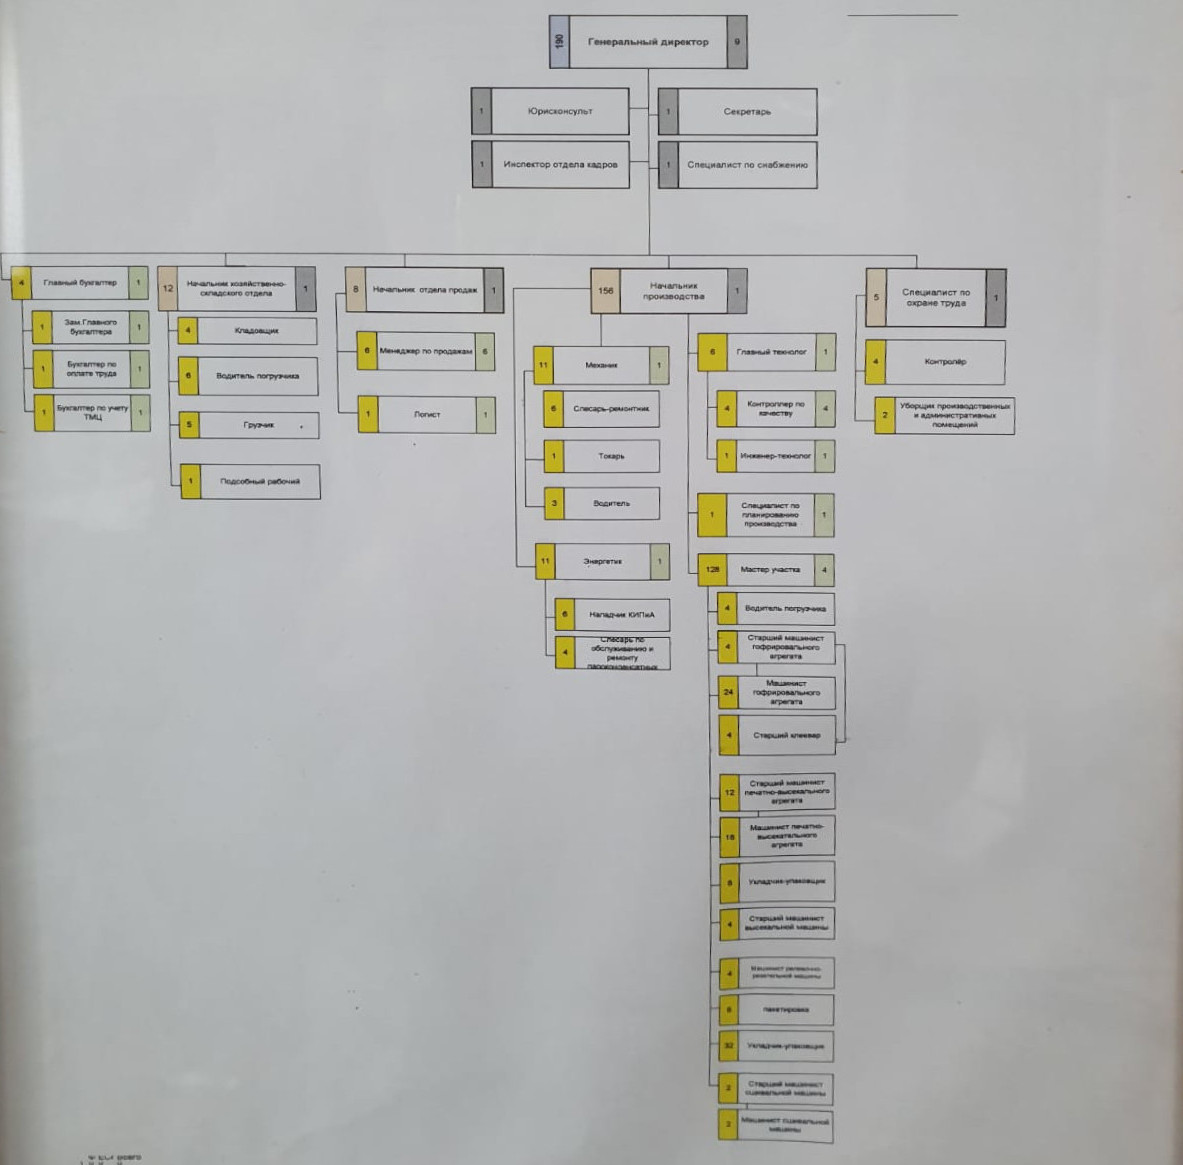
\includegraphics[
  width=1\textwidth, height=1\textheight, 
  angle=0, keepaspectratio]{Pics/OrgChart.jpg}
\end{center}
  \caption{Организационная структура производства.}
  \label{pic:orgchart}
\end{figure}
\clearpage

% \begin{figure}
% \begin{center}
%   \includegraphics[
%   %width=\textwidth, height=1\textheight, 
%   angle=90, keepaspectratio]{Pics/Structure3.png}
% \end{center}
%   \caption{Организационная структура производства. Продолжение}
%   \label{pic:structure}
% \end{figure}
% \clearpage


%%\begin{figure}
%\begin{center}
%\ifnum\pdfoutput=0
%  \includegraphics[40,0][366,292]{Pics/structure.png}
%\else 
%  \includegraphics[height=0.94\textheight, keepaspectratio]{Pics/00_Структура.jpg}
%\fi
%\end{center}
%  \caption{Оргштатная структура АО ''Новосибирский КБК''}
%  \label{pic:structure}
%\end{figure}

\clearpage

\section{Территориальное расположение}
%

Местонахождение ПРЕДПРИЯТИЯ --- \CURADDRESS.

Адрес производства:
\ADDRESS.




\section{Описание производственных процессов}

%%\documentclass[12pt,russianb]{report}
%\usepackage[russian]{babel}
%\usepackage[cp1251]{inputenc}


\documentclass{report}
\usepackage[T2A]{fontenc}
\usepackage[utf8]{inputenc}
\usepackage[english,russian]{babel}

\usepackage{longtable}   % подключение длинных таблиц
\usepackage[dvipsnames]{xcolor}
\usepackage{multirow}
\usepackage{array}
\usepackage{indentfirst} % идентификация первых абзацев после секционирования
\usepackage{lastpage}    % пакет достчета страниц 

\usepackage{fancyhdr}                    % расширенный формат страниц
\voffset=-25mm   % -25                   % сдвиг страницы вверх
\hoffset=-15mm   % -10     


  \usepackage[pdftex]{graphicx}            % загрузка графики под pdf
  \usepackage{cmap}                        % чтоб работал поиск по PDF 
  \usepackage[unicode, pdftex, colorlinks, linkcolor=blue]{hyperref}   % гиперссылки в PDF
  \pdfcompresslevel=9                      % сжимаем PDF 
  \textheight=240mm                        % для PDF высота печатного текста
  \textwidth=165mm                         % ширина печатного текста
  \renewcommand{\baselinestretch}{1.3}        % для PDF интервалы между
  \baselineskip=1.3\baselineskip              % строками 


\pagestyle{empty}
\pagestyle{fancy}
\lhead{\tiny ООО <<Опти-Софт>>}
\chead{}
\rhead{\tiny Отчет по обследованию производства \FIRMA}
\cfoot{\rule{\textwidth}{0.25pt}
~\arabic{page}}

\sloppy                             % подавление дополнительных переносов
\righthyphenmin=2                   % можно переносить
\setlength{\parindent}{10mm}        % отступ красной строки

\usepackage{todonotes}
%\newcommand{\todo}[1]{}
%\renewcommand{\todo}[1]{{\color{red} TODO: {#1}}}



\usepackage{placeins}    % пакет позволяет вставлять плавающие объекты (рисунки) в том месте, 
                         % где это необходимо. Для вывода рисунка после него встаить команду \FloatBarrier
                         
                         
                         

\newcommand{\red}[1]{\textcolor{Red}{#1}}
\newcommand{\green}[1]{\textcolor{Green}{#1}}
\newcommand{\blue}[1]{\textcolor{Blue}{#1}}                       
\newpage

\subsection{Управление взаимоотношениями с клиентами}
\label{BP_CRM}

Поиском новых клиентов занимаются менеджеры отдела продаж.

Менеджеры ищут новых клиентов в различных открытых источниках, через обзвон потенциальных покупателей, через Интернет, систему 2Gis.
Менеджеры для поиска новых клиентов используют холодные звонки, выставки.

% Для продаж выделено 4 менеджера и 2 инженера по отгрузке.

CRM системы не выявлено.
Новых клиентов каждый менеджер ведет в своих файлах, блокнотах. Единой базы потенциальных покупателей не выявлено.

Новых клиентов бухгалтер заводит в справочник Контрагенты в системе 1С:УПП только при заключении договора.


В отделе продаж работает шесть человек: старший, ведущий, младший менеджер.
Выделено три группы менеджеров. Реально создано только две группы.

% Новые клиенты заносятся как лиды. МАП заносит карточку покупателя в модуле CRM системы 1С: УНФ. МАП ведет историю взаимоотношений с клиентами вручную записывая историю звонков, рассылок.
% В CRM созданы шаблоны сценариев работы с покупателем. Каждое событие работы с контрагентом является  элементом справочника с тем  шаблоном.
% При появлении потенциального клиента МАП определяет лицо принимающее решение со стороны организации. МАП запрашивает требования по изготовлению изделия и получает техническое задание (размеры и характеристики нового изделия). 

% В отделе продаж есть четкий регламент работы по новым заказчикам.
% Одна сделка представляет собой несколько изделий готовой продукции для одного клиента.



Опросного листа по клиенту не выявлено.
%
Общего списка потенциальных клиентов и холодных клиентов не выявлено.
Старший менеджер ведет таблицу в Excel по потенциальным клиентам (форма \ref{pic:d3}).
%
%
%
%%
%Учет взаимоотношений с клиентами ведется на ручном уровне. Менеджеры отдела маркетинга 
%занимаются поиском и привлечением новых покупателей. Выделяется пассивный поиск через сайт, рекламу и участие в мероприятиях, и активный поиск через адресную рассылку.
%Все контакты хранятся на сетевом ресурсе в сети ПРЕДПРИЯТИЯ, куда есть доступ большинству пользователей сети.
%При появлении нового покупателя менеджеры отдела маркетинга создают каталог в сетевом каталоге клиентов.
%Внутри каталога хранится информация по письмам с клиентами, договорам, спецификациям и тендерам.
%
%%
%Новых заказчиков ведет менеджер отдела продаж и закупок.
%После выполнения предварительных заказов заказчику ведущий специалист отдела продаж передает клиентов менеджерам отдела продаж.
%%
%%\begin{figure}
%%\begin{center}
%%\ifnum\pdfoutput=0
%%  \includegraphics[40,0][366,292]{Pics/TK1.png}
%%\else 
%%  \includegraphics[height=0.94\textheight, keepaspectratio]{Pics/CustomerList.jpg}
%%\fi
%%\end{center}
%%  \caption{Разделение потребителей гофротары в разрезе маркетологов}
%%  \label{pic:CustomerList}
%%\end{figure}
%%\clearpage
%%
%%
\begin{figure}
\begin{center}
 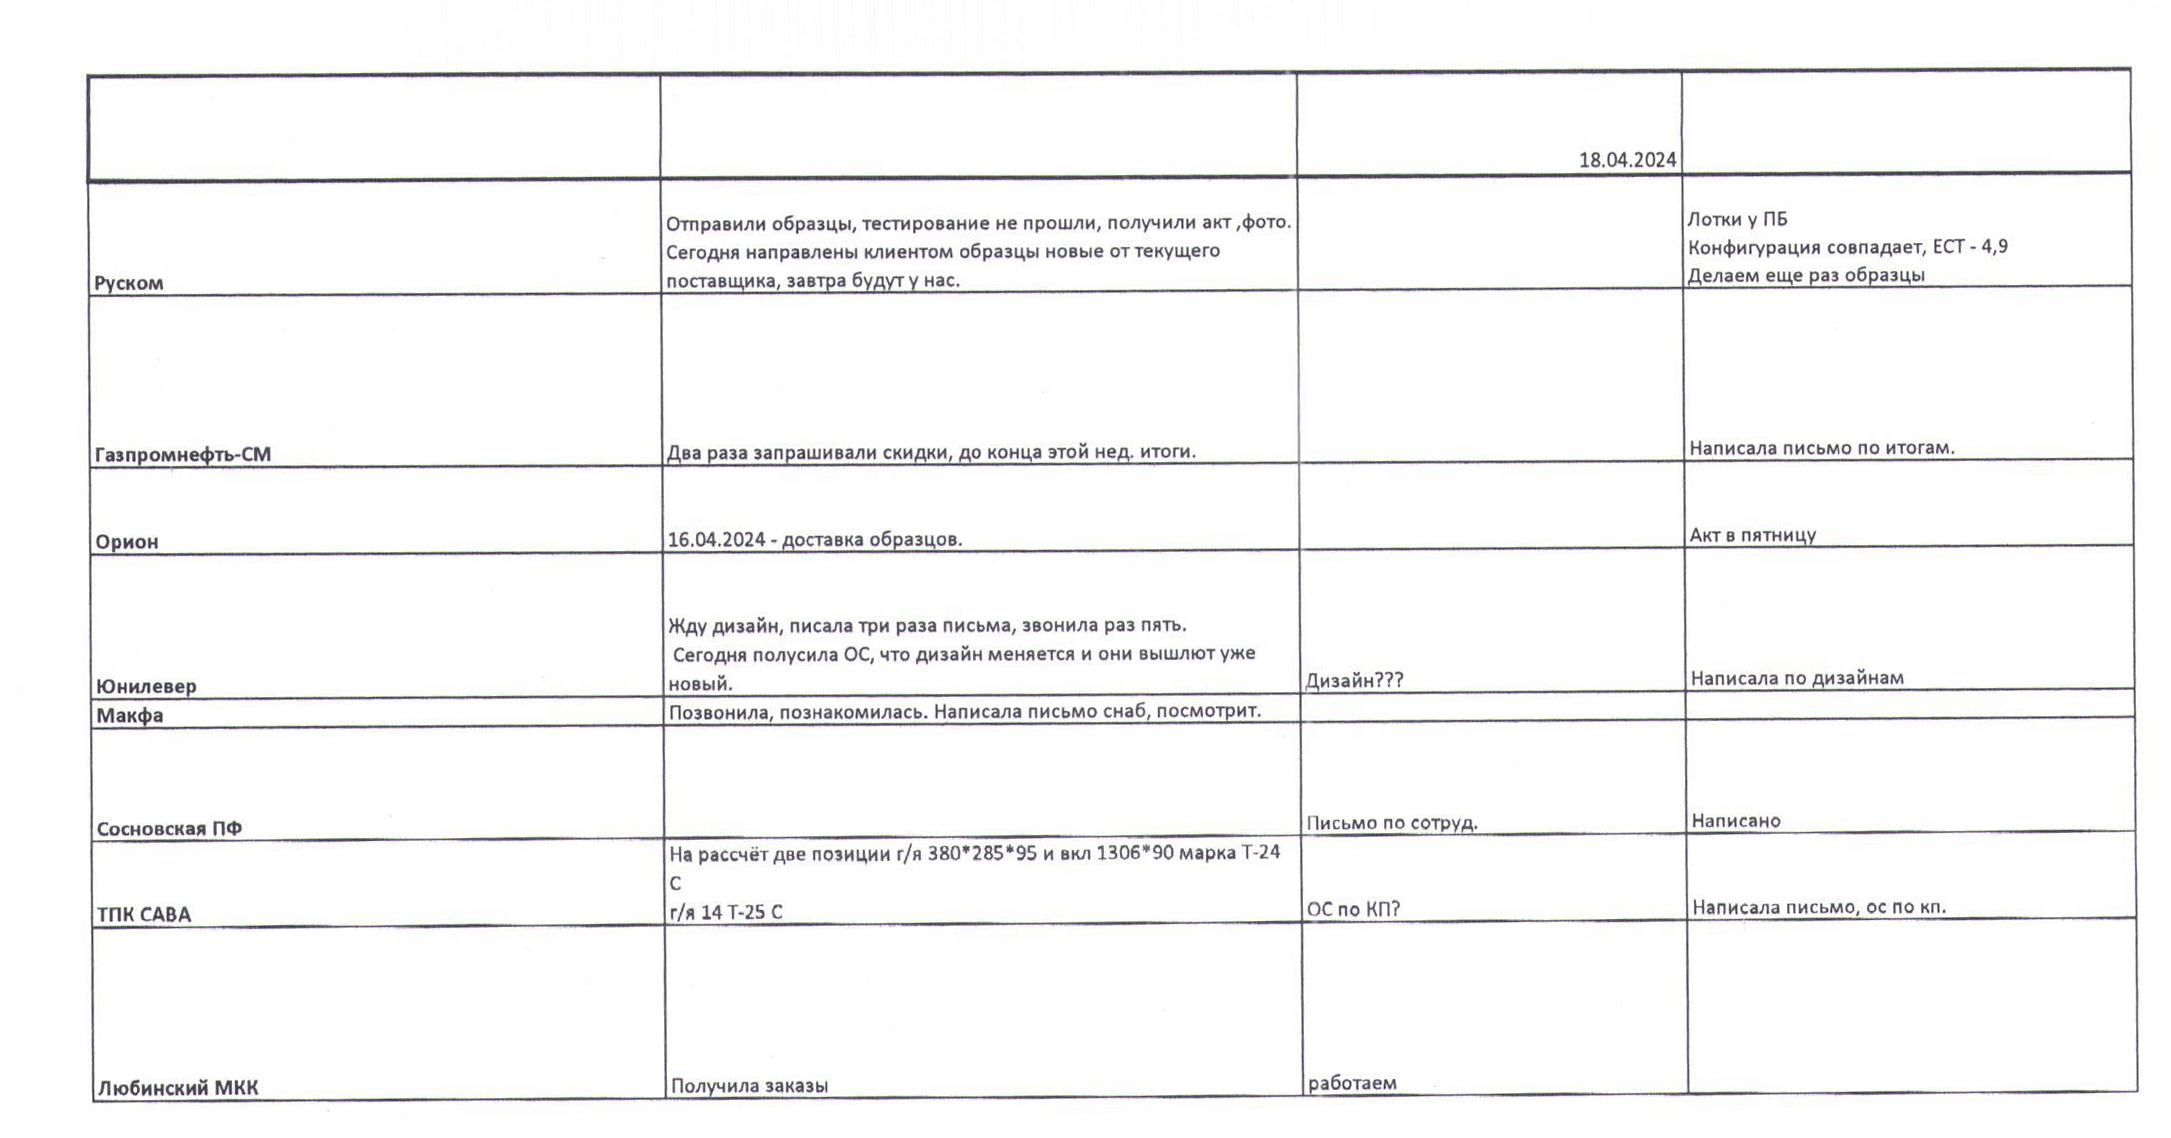
\includegraphics[height=0.5\textheight, angle=90, keepaspectratio]{Pics/d03.jpg}
\end{center}
 \caption{Список потенциальных покупателей}
 \label{pic:d3}
\end{figure}
\clearpage
%
%


\clearpage
\ifx \notincludehead\undefined
\normalsize
\end{document}
\fi 
\newpage
\subsection{Долгосрочное планирование продаж}
\label{bp:monthplan}

Долгосрочное (месячное) планирование продаж выполняется в отделе продаж (форма \ref{pic:d2}).
Каждый менеджер создает по своим заказчикам план продаж на будущий месяц по номенклатуре изделий и в количественном выражении. 
План нужен для руководства и для долгосрочного планирования сырья.

% Коммерческий директор контролирует выполнение  плана продаж по отчету ''План продаж'' (рис. \ref{pic:d3}).
% Каждый понедельник все менеджеры формируют в таблице MS Excel план поступления денежных средств для коммерческого директора.





%Менеджеры ведут месячный план продаж в формате MS Excel.
%%План формируется стоимостных (тыс. руб.) показателях.
%Форма плана приведена на рис. \ref{pic:monthplan}.  

%Годовой план продаж разрабатывается коммерческим директором ООО ''ТД «Брянский картон'' и является целевым показателем для других подразделений производства (см. рис. \ref{pic:monthplan}).
%План является необходимым ограничением для менеджеров отдела продаж на год. План формируется в стоимостных (тыс. руб.) показателях.
% 
\begin{figure}
\begin{center}
 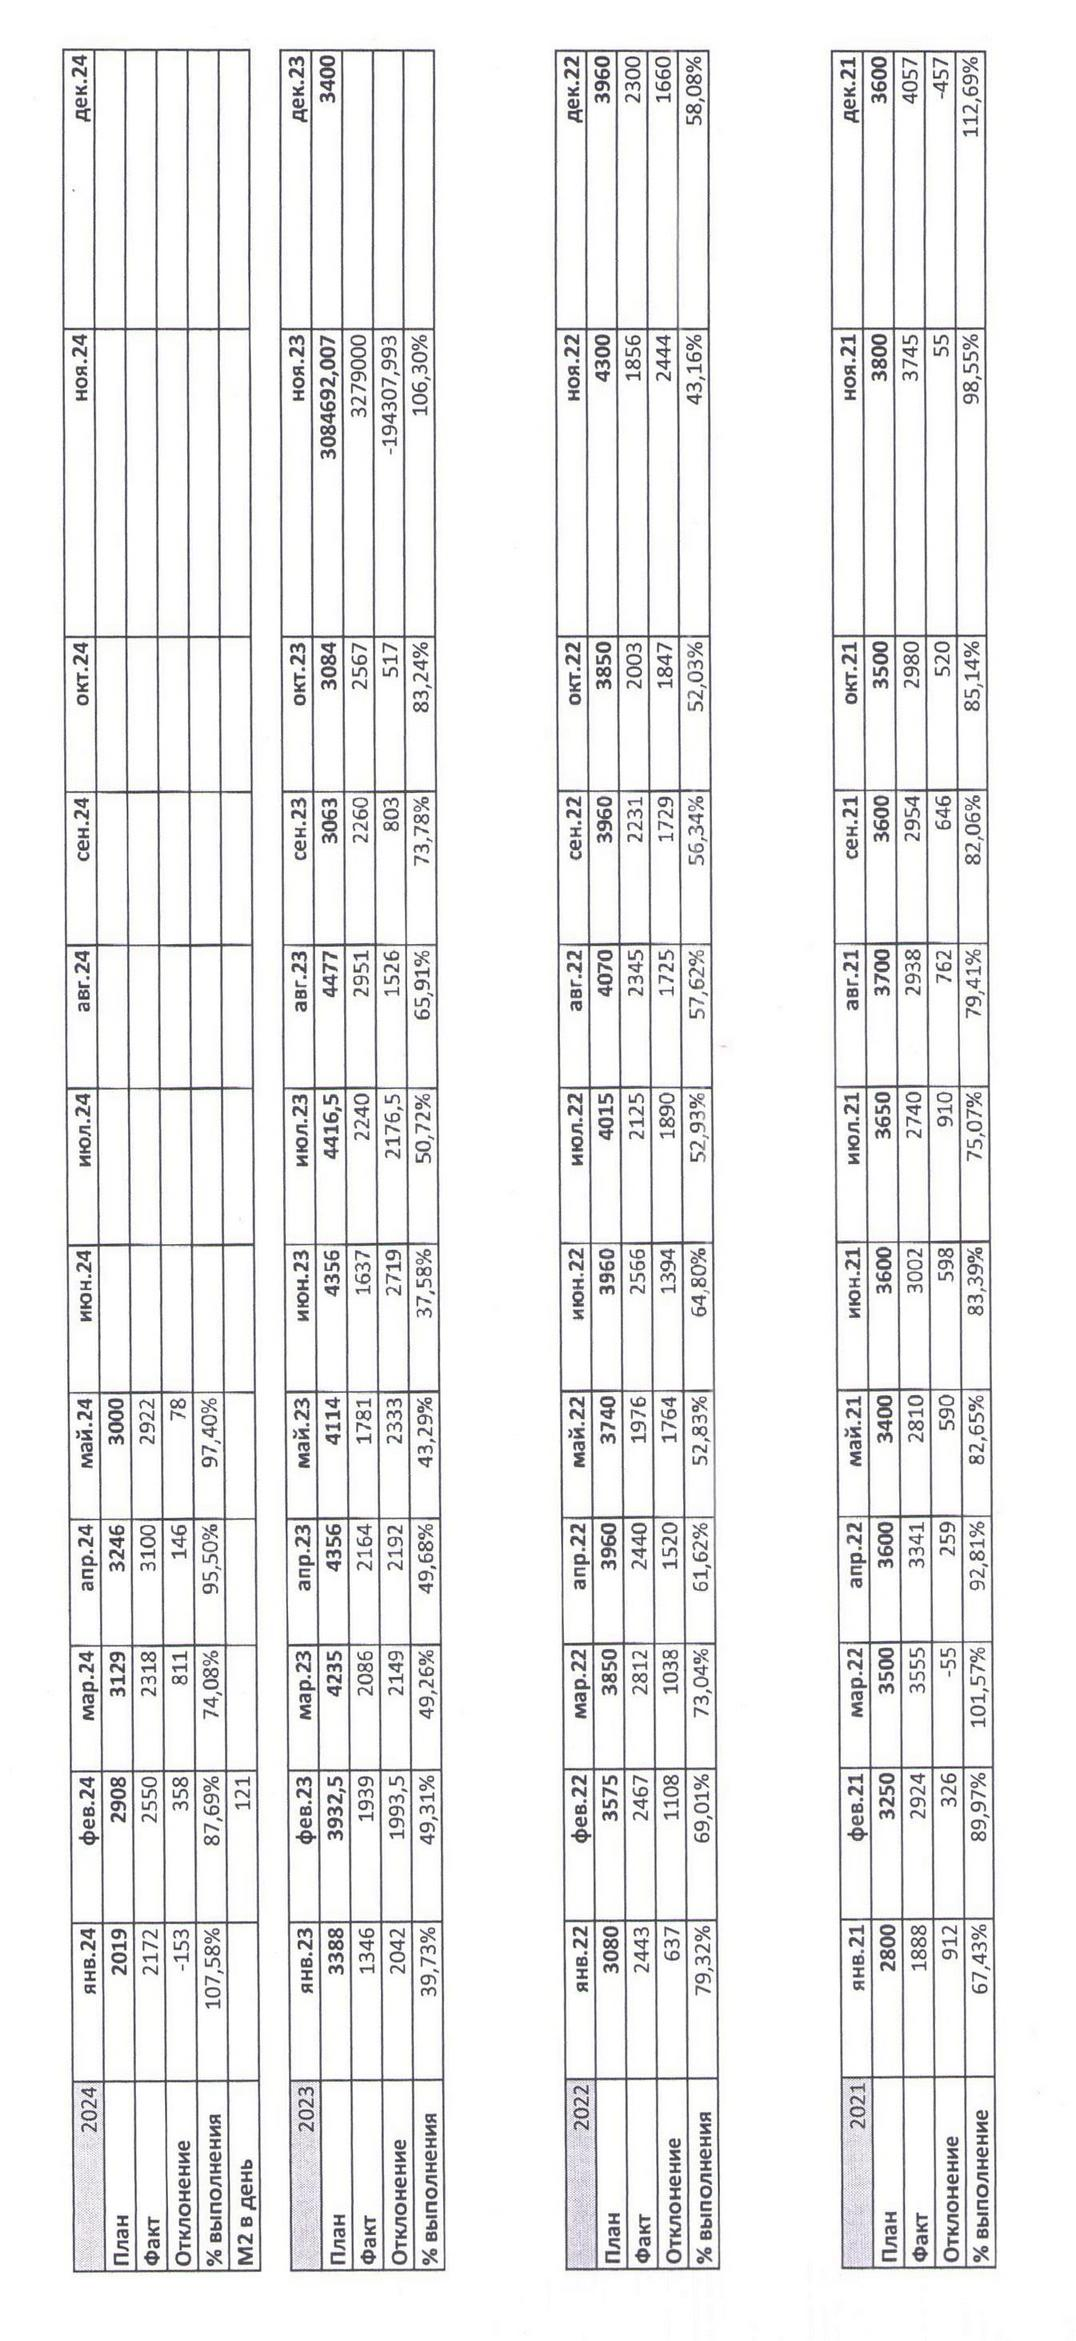
\includegraphics[height=0.8\textheight, width=1.3\textwidth, angle=0, keepaspectratio]{Pics/d02.jpg}
\end{center}
 \caption{Готовой план продаж}
 \label{pic:d2}
\end{figure}
\clearpage


\ifx \notincludehead\undefined
\normalsize
\end{document}
\fi
\newpage
\subsection{Оперативное планирование продаж}
\label{bp:salesplan}




Генеральный директор даёт ограничение по плану продаж на каждый месяц.
В системе 1С:УПП создается оперативный продаж на каждый месяц (см. \ref{pic:d1}).
План продаж определяет генеральный директор.
В форме представлены плановые показатели по продажам, фактическая величина отгрузки, просроченная задолженность по покупателю.


% При появлении от клиентов заявок от покупателей менеджеры регистрируют в системе СБИС документ ''Заявка покупателя'' (рис. \ref{pic:dd9}). Менеджеры формируют при необходимости счет на оплату из формы документа \ref{pic:dd8} или создают документ «Счет». 

% В системе СБИС менеджеры регистрируют все заявки покупателя.

% %Выделено несколько крупных покупателей, по которым до 25 числа каждого месяца требуется создавать заявки покупателей в 1С: УПП. Таких клиентов только 50\%. 
% Составление списка заявок покупателей в системе СБИС 
% % на начало месяца 
%  можно условно назвать 
% % является 
% оперативным планирование продаж.
% %
% %






%Ежемесячно менеджеры отдела сбыта и логистики совместно с коммерческим директором разрабатывают оперативный план. 

% Разрез планирования: виды выпускаемой продукции, декада месяца.
% Показатель планирования: метры квадратные по готовой продукции.
 
%Позаказный учет отсутствует.
 
%Для каждой позиции указывается заказчик, размеры изделия, марка, оснастка, композиция сырья, план в производство и факт производства и отгрузки.

%План создается по каждому менеджеру. Оперативный план продаж является документом, по которому формируются все дальнейшие планы: план производства, план работы гофроагрегата, план работы перерабатывающих линий, план потребности в материалах, план отгрузки.
%Форма плана приведена на рис. \ref{pic:salesplan}.
%
\begin{figure}
\begin{center}
 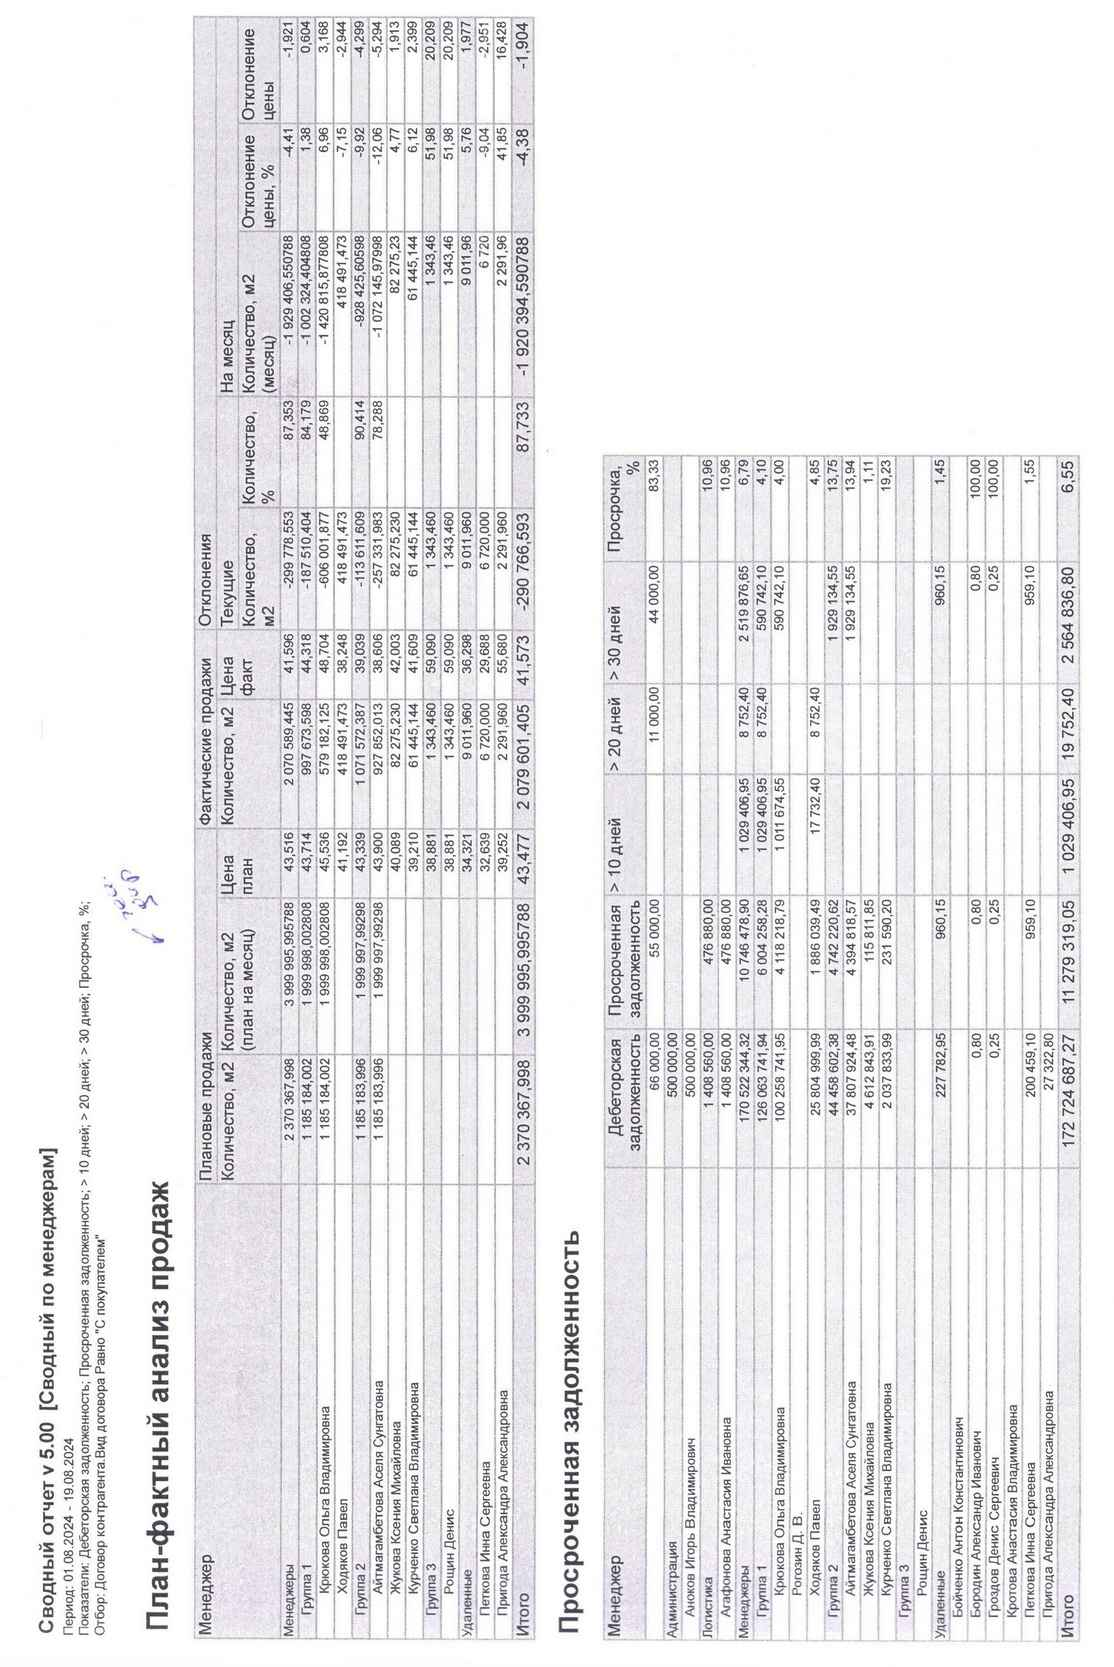
\includegraphics[height=0.94\textheight, width=0.9\textwidth,  keepaspectratio]{Pics/d01.jpg}
\end{center}
 \caption{План продаж на месяц по каждому менеджеру}
 \label{pic:d1}
\end{figure}
\clearpage


% \begin{figure}
% \begin{center}
%  \includegraphics[height=0.94\textheight, width=0.9\textwidth,  keepaspectratio]{Pics/pic.jpg}
% \end{center}
%  \caption{Цепочка заказов для планирования}
%  \label{pic:pic_d14}
% \end{figure}
% \clearpage

%
%



%Оперативное планирование определяется на основе формы \ref{pic:monthplan}, куда менеджер фиксирует все поступающие заявки.
%Производство каждый день  сообщает менеджерам коммерческого отдела  результаты работы производства. 
%При этом плановик  звонит менеджеру коммерческого отдела и говорит какие заказы приняты в производство на текущую дату.
%%Специалисты отдела планирования сообщают план выполнения на 2 дня. 
%Планировщик сообщает дату, на которую поставлен заказ. Так менеджеры узнают, когда их заявка покупателя поставлена в работу. 
%Дата (период) производства в форме плана  (см рис. \ref{pic:monthplan}) уже согласована.
%В программе 1С менеджер создает надокумент ''Счет''  и печатает форму заказа на отгрузку, в котором указывает дату отгрузки, адрес доставки, номенклатуру продукции, цены, объём. 


%\begin{figure}
%\begin{center}
%  \includegraphics[height=0.94\textheight, keepaspectratio]{Pics/prodline_loading.jpg}
%\end{center}
%  \caption{Отчет по загруженности линий}
%  \label{pic:prodline_loading}
%\end{figure}

\clearpage
\ifx \notincludehead\undefined
\normalsize
\end{document}
\fi
\newpage
\subsection{Расчет предварительной стоимости продукции}
\label{bp:calculation}


Менеджер собирает всю информацию от клиента по новому изделию. 
Менеджер получает требования от клиента, уточняет размеры, условия доставки, марки. Требования обычно приходят устно, через мессенджеры, почту.

В систему 1С:УПП заведено пять обезличенных клиентов и для расчёта цены, которых используют менеджеры.

Менеджер создаёт в системе  1С:УПП  заказ покупателя, создаёт номенклатуру в системе (рис. \ref{pic:d05}), выполняет расчет цены на номенклатуру (рис. \ref{pic:d05}),  выбирает маршрут (рис. \ref{pic:d06}).

Транспорт используется только наёмный.  Для доставки по городу используется собственный автомобиль предприятия Газель.
Менеджер создаёт бизнес карту в системе 1С:УПП,  указывает вариант доставки, отсрочку платежа. Система 1С:УПП рассчитывает минимальную цену продажи. Менеджер указывает процент рентабельности и получает цену продажи.

Далее менеджер формирует коммерческое предложение в Word вручную с указанием рассчитанной цены.
Менеджер отправляет коммерческое предложение клиенту на согласование.
После согласования цены менеджер старается изготовить образцы готовой продукции.




Менеджер высылает коммерческое предложение клиенту.  Заказчик в ответ высылает менеджеру согласованное предложение с реквизитами для заключения договора. 
%Менеджер формирует договор поставки и высылает заказчику на согласование.

После согласования коммерческого предложения Менеджер 
создает вручную проект договора и  спецификацию к договору. 

% Номер договора присваивает юрист по запросу менеджера. 
Менеджер в системе 1С:УПП создает номенкатуру по клиенту, заводит в справочник Номенклатура в 1С:УПП новую позицию, указывает размеры, площадь, тип гофры, цвет картона, размеры упаковки.
Система 1С:УПП присваивает номенклатурный номер.
Менеджер создает бланк договора и спецификацию в формате MS Word. 
Менеджер создает при условиях предоплаты счет в в системе 1С:УПП. 
Менеджер печатает счет на оплату при необходимости.

Менеджер отправляет клиенту договор с приложением в виде спецификации, счет на предоплату при необходимости.
Клиент подписывает договор, спецификацию и оплачивает счет.



После согласования цены Менеджер должен начать разработку ТК (см. процесс ''Подготовка производства'' \ref{bp:Prepare}).


% Для расчета цены менеджер использует шаблон в MS Excel (рис. \ref{pic:pic_d2}). 
% К цене сырья добавляется стоимость на сложную высечку.  Стоимость упаковки включена в цену изделия. Таким образом менеджер определяет базовую нормативную себестоимость продукции.  Цена продажи определяется менеджером исходя из себестоимости и рентабельности производства.


% Каждый менеджер ведет расчет по новым изделиям в своих файлах. Менеджер заносит в файл наименование изделия (обычно контрагент) длину, ширину, высоту (внутренние размеры изделия). По формуле будет рассчитана площадь изделия. Менеджер выбирает сырье по композиции. 
% Менеджер подбирает сырье по аналогии либо по истории такой же коробки. 

% При необходимости изготовления сложной высечки менеджер  запрашивает у контрагента чертеж или образец (процесс ''Изготовление образцов продукции'' \ref{bp:pattern}).

% На основании расчета (рис. \ref{pic:pic_d2}) менеджер формирует коммерческое предложение (рис. \ref{pic:pic_d3}). Для печати предложения используется шаблон.
% На основе полученного результата расчета себестоимости изделия менеджер  формирует коммерческое предложение и высылает его заказчику (рис. \ref{pic:pic_d3}). Для печати предложения используется шаблон. Номер КП указывается по порядку. В коммерческом предложении указывается наименование гофропродукции, марка, профиль и цена изделия. Цена актуальна в течение месяца. 
% Коммерческое предложение высылается заказчику для согласования.
% Все предложения менеджер фиксирует в таблице MS Excel предложения  (рис. \ref{pic:pic_d4}).


% Менеджер высылает КП заказчику.
% Заказчик высылает менеджеру согласованное предложение с реквизитами для заключения договора. Менеджер формирует договор поставки и высылает заказчику на согласование. В дополнение к договору менеджер формирует спецификацию на цену продукции, где указывается согласованный перечень поставляемой продукции и цены на нее (рис. \ref{pic:pic_d5}). Дополнительное соглашение является дополнением к договору. Все документы заполняются менеджером вручную.
% После согласования заказчиком коммерческого предложения менеджер запрашивает карточку контрагента для заключения договора. Менеджер отправляет в офис Московский карточку контрагента и спецификацию (рис. \ref{pic:pic_d5}) для заключения договора.

% Секретарь формирует договор с заказчиком, присваивает номер дату и высылает договор менеджеру по электронной почте. Менеджер согласует договор с заказчиком. Заказчик подписывает договор. Менеджер передает в бухгалтерию карточку заказчика и копию подписанного договора. 
% Отдел учета в системе 1С Предприятие 7.7 Бухгалтерия  создаёт  справочнике ''Контрагенты'' нового заказчика и договор.

% После выставления счета менеджер контролирует оплату от заказчика. Контроль оплаты менеджер выполняет в программе 1С 7.7. Бухгалтерия. В системе 1С 8.3 ''Бухгалтерия предприятия'' ведётся  учет поступления денежных средств на расчётный счёт, но с опозданием.
% Банк ведется в двух системах: 1С 7.7. Бухгалтерия и 1С 8.3 ''Бухгалтерия предприятия''.


%Менеджер получает запрос только по почте менеджер создает заявку на расчёт \ref{pic:calculation1}.
%Менеджер звонит на производство специалисту по планированию, который присваивает номер гофроизделия в файле "Начало".
%Менеджер подбирает сырье для производства изделия самостоятельно, при это есть таблица компоновок сырья \ref{pic:Layerscost}, которая не используется. Менеджер определяет количество на поддоне. При указании вида транспорта менеджер рассчитывает стоимость доставки \ref{pic:transportcost}. Менеджер рассчитывает количество поддонов, чтобы посчитать затраты на доставку. Особые условия указанной в условиях упаковке.
%
%Файл  \ref{pic:calculation1} отправляется экономисту почтой. 
%
% Расчет предварительной стоимости изделия выполняет МАП в системе 1С:УНФ при получении заявки от покупателя. Цена для продажи рассчитывается исходя из суммы следующих слагаемых.
% \begin{itemize}
% \item Стоимость гофрокартона -- рассчитывается как стоимость одного метра гофрокартона определенного профиля.
% \item Наценка за печать -- менеджер указывает примерную площадь запечатки краской в процентах. Процент запечатки учитывается при расчете затрат на печать.
% \item Паллетирование -- если для изделия требуется укладка на поддон, то стоимость паллетирования добавляется в стоимость изделий. Стоимость паллетирования одного изделия рассчитывается как стоимость паллетирования одного поддона, деленная на количество изделий на поддоне.
% \item Затраты на упаковку;
% \item Транспортировка -- стоимость доставки готовой продукции до получателя на единицу продукции.
% \end{itemize}
%
%
\begin{figure}
\begin{center}
  \includegraphics[width=\linewidth, height=0.94\textheight, keepaspectratio]{Pics/d04.jpg}
\end{center}
  \caption{Форма расчета стоимости нового изделия}
  \label{pic:d04}
\end{figure}
\clearpage
%
%
\begin{figure}
\begin{center}
  
\includegraphics[width=\linewidth, height=0.94\textheight, keepaspectratio]{Pics/d05.jpg}
\end{center}
  \caption{Форма создания новой номенклатуры}
  \label{pic:d05}
\end{figure}
\clearpage

%
%%
\begin{figure}
\begin{center}
  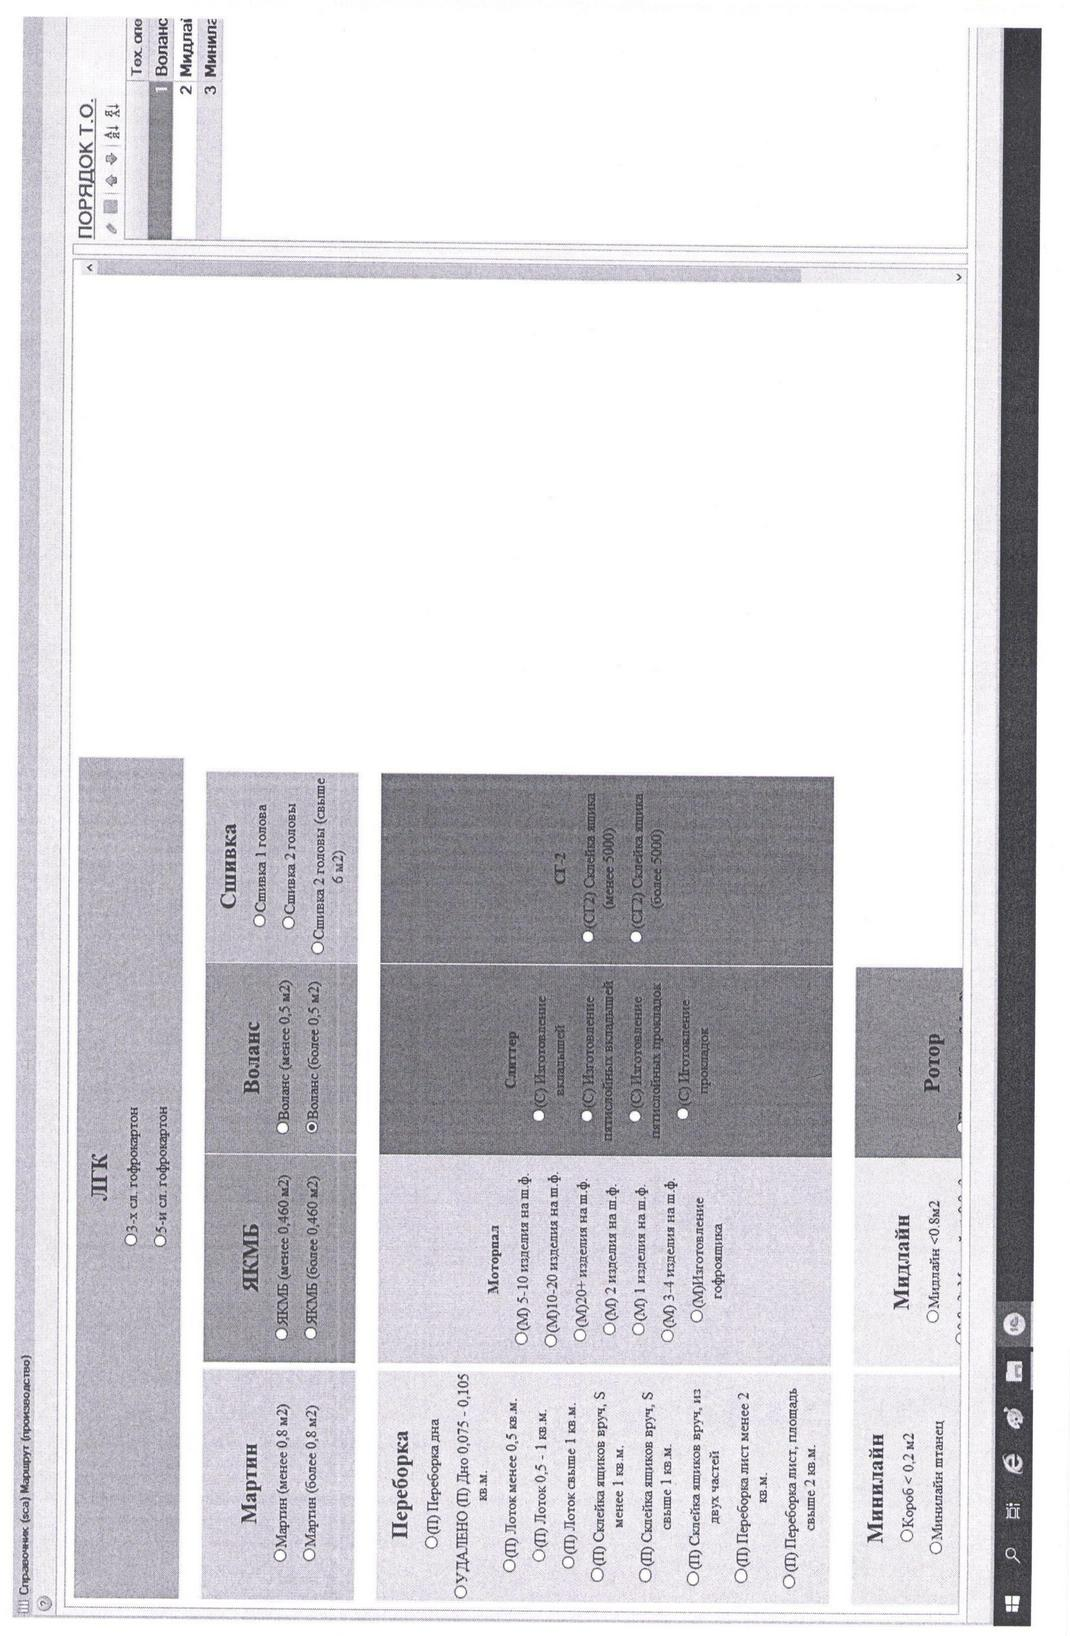
\includegraphics[width=\linewidth, height=0.94\textheight, keepaspectratio]{Pics/d06.jpg}
\end{center}
  \caption{Форма выбора маршрута изготовления продукции}
  \label{pic:d06}
\end{figure}
\clearpage


% \begin{figure}
% \begin{center}
%   \includegraphics[width=\linewidth, height=0.94\textheight, keepaspectratio]{Pics/d6.jpg}
% \end{center}
%   \caption{Форма спецификации к договору}
%   \label{pic:d6}
% \end{figure}
% \clearpage

% \begin{figure}
% \begin{center}
%   \includegraphics[width=\linewidth, height=0.94\textheight, keepaspectratio]{Pics/pic_d5.jpg}
% \end{center}
%   \caption{Форма спецификации к договору}
%   \label{pic:pic_d5}
% \end{figure}
% \clearpage

%
%\begin{figure}
%\begin{center}
%\ifnum\pdfoutput=0
%  \includegraphics[40,0][366,292]{Pics/03_calculation2.png}
%\else 
%  \includegraphics[width=\linewidth, height=0.94\textheight, keepaspectratio]{Pics/03_calculation2.jpg}
%\fi
%\end{center}
%  \caption{Расчет стоимости изделия от экономиста.}
%  \label{pic:calculation2}
%\end{figure}
%\clearpage
%
%
%\begin{figure}
%\begin{center}
%\ifnum\pdfoutput=0
%  \includegraphics[40,0][366,292]{Pics/03_calculation3.png}
%\else 
%  \includegraphics[width=\linewidth, height=0.94\textheight, keepaspectratio]{Pics/03_calculation3.jpg}
%\fi
%\end{center}
%  \caption{Упрощенный расчет стоимости.}
%  \label{pic:calculation3}
%\end{figure}
%\clearpage
%
%
%

%
%
%\begin{figure}
%\begin{center}
%\ifnum\pdfoutput=0
%  \includegraphics[40,0][366,292]{Pics/04_KP1.png}
%\else 
%  \includegraphics[width=\linewidth, height=0.94\textheight, keepaspectratio]{Pics/04_KP1.jpg}
%\fi
%\end{center}
%  \caption{Коммерческое предложение.}
%  \label{pic:KP1}
%\end{figure}
%\clearpage
%
%
%\begin{figure}
%\begin{center}
%\ifnum\pdfoutput=0
%  \includegraphics[40,0][366,292]{Pics/34_contract.png}
%\else 
%  \includegraphics[width=\linewidth, height=0.94\textheight, keepaspectratio]{Pics/34_contract.jpg}
%\fi
%\end{center}
%  \caption{Договор поставки.}
%  \label{pic:contract}
%\end{figure}
%\clearpage
%
%
%\begin{figure}
%\begin{center}
%\ifnum\pdfoutput=0
%  \includegraphics[40,0][366,292]{Pics/07_specification_for_contract.png}
%\else 
%  \includegraphics[width=\linewidth, height=0.94\textheight, keepaspectratio]{Pics/07_specification_for_contract.jpg}
%\fi
%\end{center}
%  \caption{Спецификация к договору поставки.}
%  \label{pic:specificationforcontract}
%\end{figure}
%\clearpage
%
%
%
%
%
%
%
%
%
%
%%Расчет предварительной стоимости изделия выполняется в отделе маркетинга при получении заявки от покупателя.
%%
%%Технолог ОМ заполняет таблицу по расчету предварительной себестоимости изделия (см. рис.\ref{pic:Calculation}. Экономист в структуре ОМ выполняет по данному расчету расчет себестоимости изделия для покупателя. Для расчета используются нормативные цены для расчета стоимости изделия (см. рис. \ref{pic:Compound},  \ref{pic:CompoundPrint}, \ref{pic:CalculationPack}, \ref{pic:CompoundPrint}).
%%
%%На основе полученного результата расчета себестоимости изделия менеджер ОМ формирует коммерческое предложение и высылает заказчику. Согласованное заказчиком предложение с реквизитами для заключения договора покупатель высылает в ОМ. Менеджер передает заявку юристу для составления и согласования договора. Экономист в структуре ОМ формирует спецификацию к договору. В спецификации указывается условия производства, отгрузки и поставки продукции (См. рис. \ref{pic:Offer}).
%%
%%На основании согласованной с заказчиком и подписанной заявки технологи ОМ разрабатывают технологическую карту изделия (см. процесс ''Подготовка производства'' \ref{bp:Prepare}).
%
%%\begin{figure}
%%\begin{center}
%%  \includegraphics[height=0.94\textheight, keepaspectratio]{Pics/Calculation.jpg}
%%\end{center}
%%  \caption{Форма заполнения расчета для нового изделия}
%%  \label{pic:Calculation}
%%\end{figure}




% \begin{figure}
% \begin{center}
%  \includegraphics[height=0.4\textheight, keepaspectratio]{Pics/dd8.jpg}
% \end{center}
%  \caption{Форма счета}
%  \label{pic:dd8}
% \end{figure}


%
\clearpage
\ifx \notincludehead\undefined
\normalsize
\end{document}
\fi
\newpage
\subsection{Управление продажами}
\label{bp:SalesManagment}


Менеджер  ведёт общий план по производству. 
Клиент высылает менеджеру заявку на изготовление продукции. 
Типовой формы заявки не выявлено.
Заявка высылается в произвольном виде по емайл, через мессенджеры. 



При поступлении заявки на изготовление продукции Менеджер в системе 1С:УПП формирует заявки покупателя (рис. \ref{pic:d11}). Менеджер создает при необходимости документ ''Счет'' на оплату из формы \ref{pic:d11}. 
Менеджер при необходимости создает в системе 1С:УПП новый договор.
Дата отгрузки в заявке является желаемой датой покупателя. 

В системе 1С:УПП есть модуль объёмно календарного планирования (рис. \ref{pic:d10}), в котором менеджер может запланировать выполнение заказа клиента.
Менеджер создаёт заказ на производство в системе 1С:УПП.
 Менеджер утверждает  в системе 1С:УПП заказ на производство (форма (рис. \ref{pic:d10}).

Менеджер проводит заказ в системе 1С:УПП.

Каждое утро в 9-00 бухгалтер в системе 1С:УПП вносит выписки из банка.
Менеджеры видят информацию по оплате покупателей в системе 1С:УПП. Каждый менеджер при необходимости обзванивает должников. 

Отдел планирования может выгружать заказы из системы 1С:УПП для оперативного планирования.

% % Менеджер заказывает заготовки точно под требуемый объем продукции и в нужный размер под готовую продукцию.
% На каждый заказ производства есть только одна заготовка.
% %Менеджер создает заказ на сторону только исходя из объема заказа на производство.
% Заказ заготовок создается точно по объему готовой продукции без дополнительных заготовок на пусконаладку. Отклонения в объеме готовой продукции прописаны в спецификациях к договору.
% % Дополнительные заготовки на пусконаладку не закупаются.
% Каждый МСЗ на основании заказа покупателя формирует заказ заготовок кратно транспортной единице (Фура). На предприятии заказывают до 12 фур в неделю заготовок. МСЗ считает загрузку транспорта вручную. Отгрузка продукции и заготовок осуществляется строго на паллетах.

% Каждое утро в 9-00 бухгалтер присылает выписки из банка. Менеджеры видят информацию по оплате покупателей в системе 1С:УНФ. Каждый менеджер при необходимости обзванивает должников. 


% Коммерческий директор ведет анализ продаж по событиям в системе 1С:УНФ.

% Покупатель может прислать дополнительную заявку кроме месячного плана.
%Все поступающие заявки менеджер фиксируют в файле “План” (см. \ref{pic:monthplan}).

%
%Менеджер может разбить заявку покупателя на части с учётом загрузки в транспорт. 

%Менеджер печатает заявку покупателя по форме \ref{pic:SalesOrder}. В форме \ref{pic:SalesOrder} есть три экземпляра: один остается у менеджера, один передается на планирование переработки, один передается на планирование раскроя.   


%Заявку распечатанную в формате MS Excel менеджер передает экономисту для проверки задолженности. Экономист ставит свой штамп на бланке при одобрении заявки. Подписанную заявку менеджер передает в плановый отдел (плановик коммерческом отделе). Экономист может запретить запуск по контролю оплаты, плохим условиям по арбитражу у контрагента. Заявка может быть не одобрена при отсутствии подписанного договора.



%
%
%\begin{figure}
%\begin{center}
%  \includegraphics[width=\linewidth, height=0.94\textheight, keepaspectratio]{Pics/prodline_loading.jpg}
%\end{center}
%  \caption{Отчет по загруженности линий.}
%  \label{pic:prodline_loading}
%\end{figure}
%\clearpage
%%

%%
%\begin{figure}
%\begin{center}
%  \includegraphics[height=0.94\textheight, keepaspectratio]{Pics/SalesOrder.jpg}
%\end{center}
%  \caption{Форма заявки покупателя}
%  \label{pic:SalesOrder}
%\end{figure}
%\clearpage


%%
%%
%%\begin{figure}
%%\begin{center}
%%\ifnum\pdfoutput=0
%%  \includegraphics[40,0][366,292]{Pics/CostRequest.png}
%%\else 
%%  \includegraphics[height=0.94\textheight, keepaspectratio]{Pics/CostRequest.jpg}
%%\fi
%%\end{center}
%%  \caption{Форма опросного листа покупателя}
%%  \label{pic:CostRequest}
%%\end{figure}
%%\clearpage
%%
%При поступлении заявки от покупателя по существующему изделию менеджер отдела продаж принимает заявку покупателя. Единого реестра заявок  не обнаружено. 
%Менеджеры отдела продаж проверяют оплату от покупателя по условиям договора.  
%Дата отгрузки это желаемая дата клиента. Дата производства по договору это дата отгрузки минус пять дней.
%Менеджер формирует заявку в формате Word и/или в программе 1С: ERP, распечатывает, подписывает, сканирует и формате pdf выкладывает на сервер для отдела планирования. 
%
%Небольшие разовые заказы менеджер по сопровождению сразу заносит в программу 1С, распечатывает, подписывает, сканирует формат PDF и выкладывает на сервер для планировщика.
%
%Появление файла сканированного в сетевом каталоге означает запуск производства заказов производством. 
%
%% 
%%При положительном решении по оплате менеджер ОСЛ создает заказ производственный. 
%%Каждый менеджер ОСЛ фиксирует заявку в портфеле заказов (см. рис. \ref{pic:WorkOrderList}).
%%
%%
%%
%%
%%\begin{figure}
%%\begin{center}
%%  \includegraphics[height=0.94\textheight, keepaspectratio]{Pics/WorkOrderList.jpg}
%%\end{center}
%%  \caption{Форма портфеля заказов по менеджеру отдела сбыта и логистики}
%%  \label{pic:WorkOrderList}
%%\end{figure}
%%\clearpage
%
%
%
%%На момент обследования любое изделие из картона на предприятии рассматривается как новое изделие. Для запуска производства менеджером отдела сбыта начинается выполнение процесса "Подготовка производства" (см. процесс \ref{BP_Prepare}).
%%
%%В систему 1С УПП менеджеры при необходимости заводят новые позиции в справочник "Контрагенты".
%%На предприятии существует стандартный прайс на продукцию (см. \ref{pic:Price}).
%%Позиции в прайсе представляют стандартные изделия, изготавливаемые на склад без заказчика.
%%
%%В отдел сбыта к менеджерам поступает заявка от заказчиков. Типовой формы заказа не существует. 
%%На основании принятой заявки от заказчика менеджер должен определить цену продажи.
%%На момент обследования любое изделие из картона на предприятии рассматривается как новое изделие. 
%%В системе 1С менеджер создает документ ''Заказ в производство'' и из программы печатает форму служебной записки (см. рис. \ref{pic:WorkOrder}).
%%Менеджер вручную заполняет требования к изделию в бланке (см. рис. \ref{pic:CostRequest}) и передает форму в отдел ТКО (см. процесс \ref{BP_Prepare}).
%%Для запуска производства менеджером отдела сбыта начинается выполнение процесса "Подготовка производства" (см. процесс \ref{BP_Prepare}).
%%
%%Одним из результатом процесса ''Подготовка производства'' является цена продажи готового изделия. Рассчитанная в ходе указанного процесса цена фиксируется в договоре на производство, указывается в счетах на оплату. Менеджер отдела сбыта формирует в системе 1С УПП форму договора с заказчикоми и счет на оплату.
%%При согласовании изделий и их цены менеджер также должен согласовать условия доставки. Доставка может осуществляться как собстсвенными силами заказчика, так и за счет исполнителя. Во втором случае условия доставки и стоимость прописываются в условиях договора и фиксируются в счете на оплату. 
%%
%%Контроль оплаты производится менеджерами на основании банковской выписки из клиент-банка или по данным бухгалтерии в системе 1С УПП. На момент обследования менеджеры пользуются банковской выпиской из программ клиент-банка.
%%
%%После подтверждения поступления оплаты менеджеры отдела продаж запускают производство. 
%%Служебная записка передается в ТКО для изготовления РРК. Комплект из служебной записки и РРК передается начальнику производства для запуска производства, запуская процесс ''Оперативное планирование'' (см. \ref{bp:OperPlan}).
%%


% \begin{figure}
% \begin{center}
%  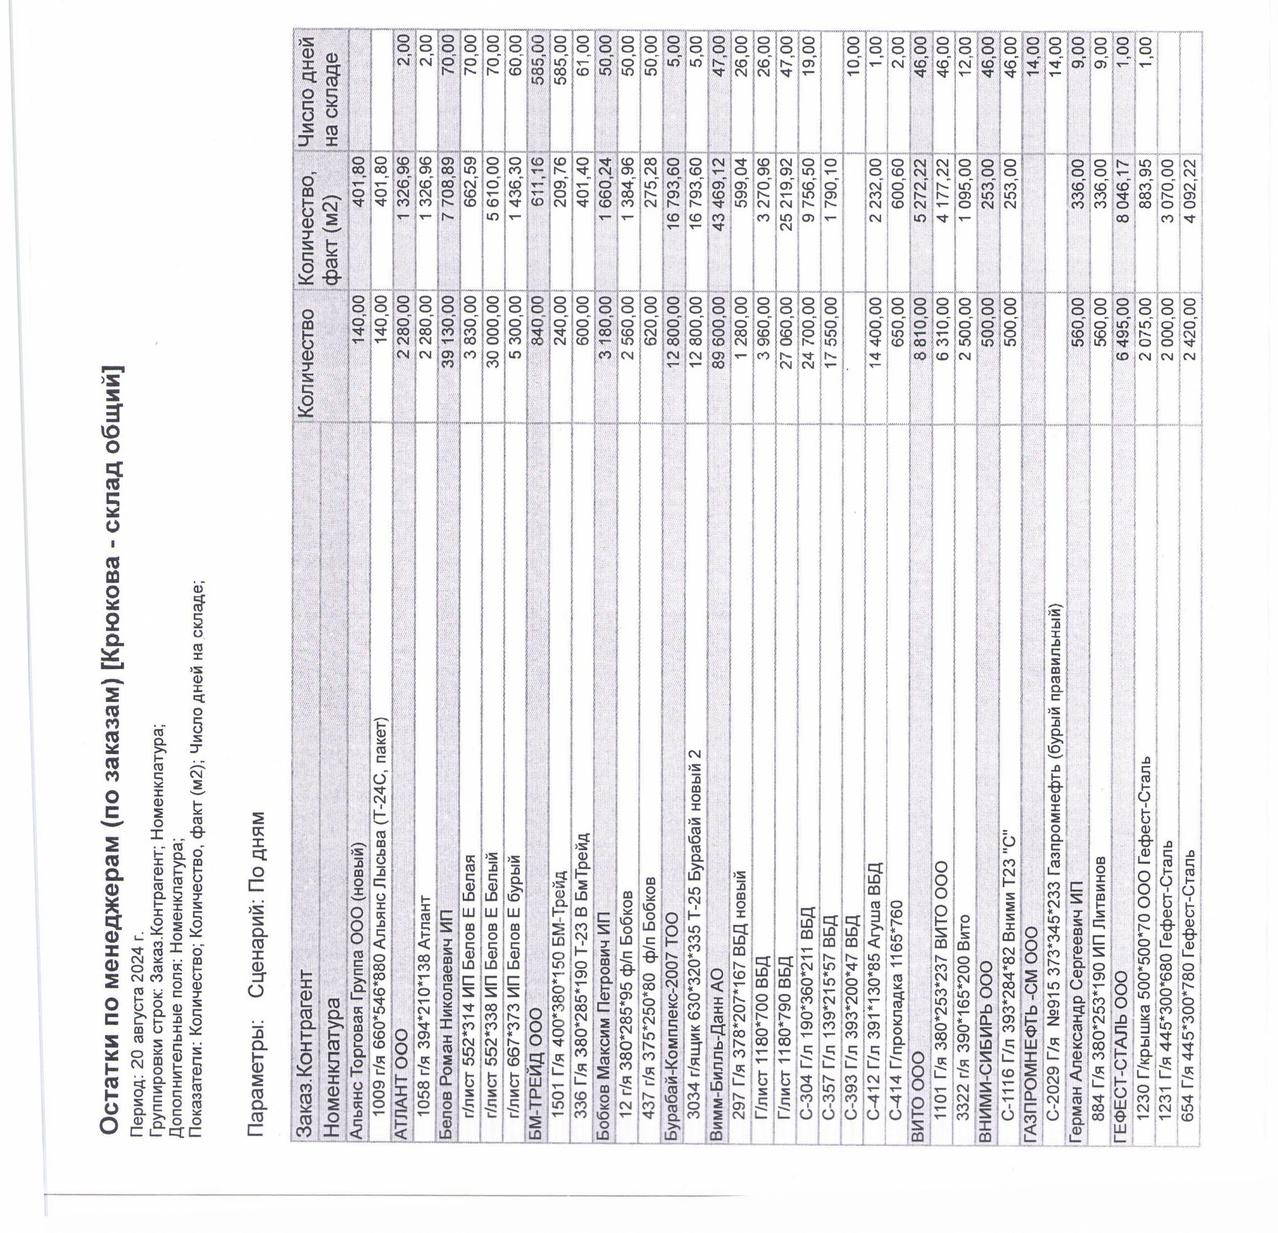
\includegraphics[height=0.4\textheight,   keepaspectratio]{Pics/d14.jpg}
% \end{center}
%  \caption{Форма заказа покупателя в системе 1С: УНФ}
%  \label{pic:d14}
% \end{figure}
% \clearpage


\begin{figure}
\begin{center}
 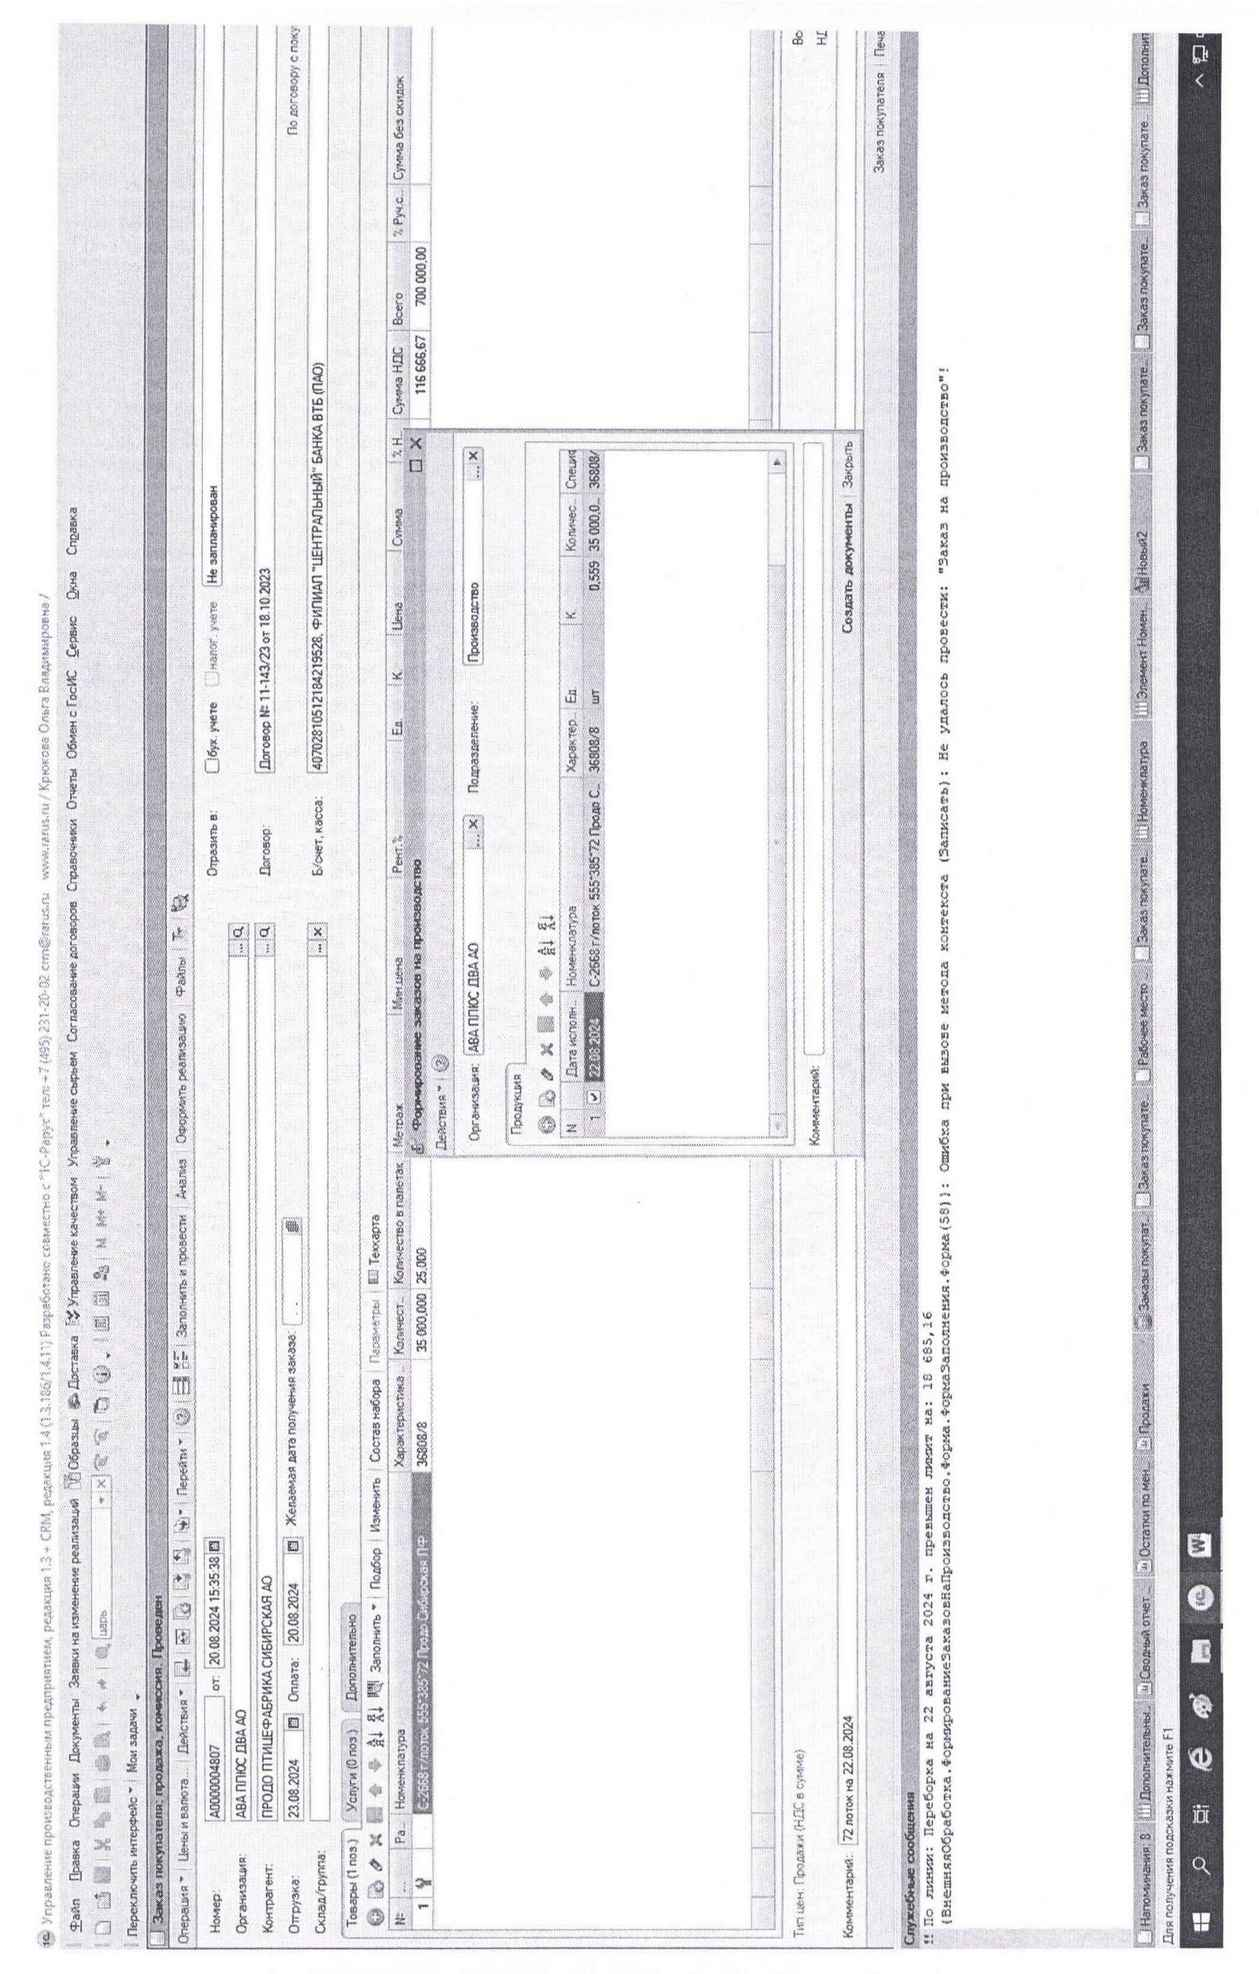
\includegraphics[height=0.8\textheight, keepaspectratio]{Pics/d11.jpg}
\end{center}
 \caption{Форма заявки покупателя в системе 1С:УПП}
 \label{pic:d11}
\end{figure}

\begin{figure}
\begin{center}
 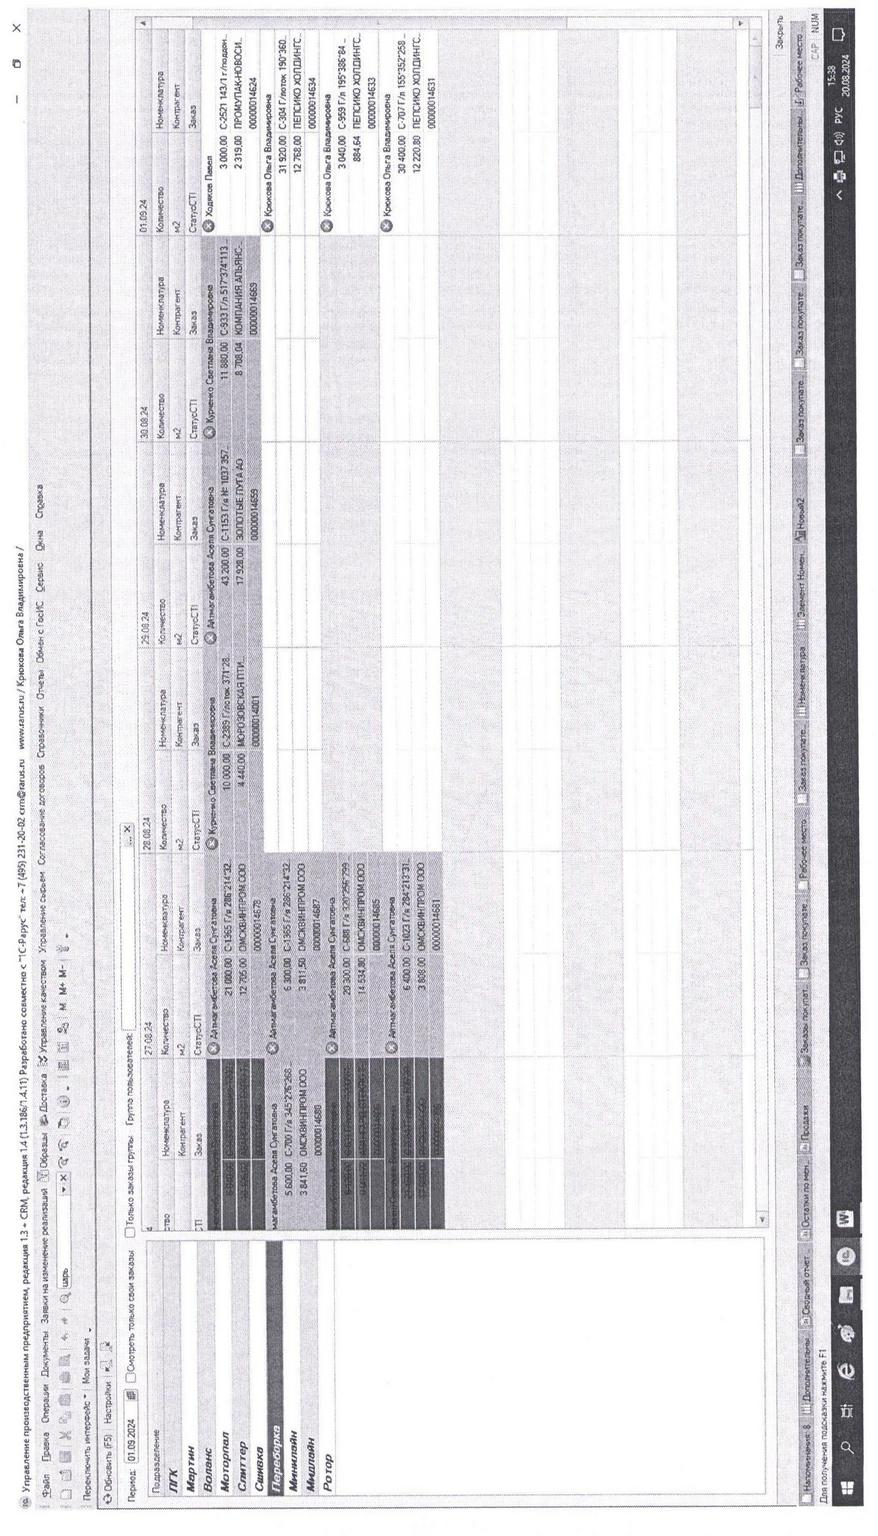
\includegraphics[height=0.8\textheight, keepaspectratio]{Pics/d10.jpg}
\end{center}
 \caption{Форма объёмно календарного планирования}
 \label{pic:d10}
\end{figure}





\clearpage
\ifx \notincludehead\undefined
\normalsize
\end{document}
\fi
\newpage
\subsection{Объемное планирование производства}
\label{bp:MonthPlan}


Месячное планирование производства строится на основании месячного планирования продаж из отдела продаж (см. процесс ''Оперативное планирование продаж'' \ref{bp:salesplan}).





% \begin{figure}
% \begin{center}
%   \includegraphics[height=0.6\textheight, angle=90, keepaspectratio]{Pics/pic_d20.jpg}
% \end{center}
%   \caption{Месячный план производства}
%   \label{pic:pic_d20}
% \end{figure}
% \clearpage


% %%
% \begin{figure}
% \begin{center}
%   \includegraphics[height=0.6\textheight, angle=90, keepaspectratio]{Pics/pic_d21.jpg}
% \end{center}
%   \caption{Месячный план с детализацией по заказам}
%   \label{pic:pic_d21}
% \end{figure}
% \clearpage


%%
%%\begin{figure}
%%\begin{center}
%%\ifnum\pdfoutput=0
%%  \includegraphics[40,0][366,292]{Pics/ProdPlan2.png}
%%\else 
%%  \includegraphics[height=0.94\textheight, keepaspectratio]{Pics/ProdPlan2.jpg}
%%\fi
%%\end{center}
%%  \caption{Месячный план производства ООО «УПП КПИ» по печатному цеху.}
%%  \label{pic:prodplan2}
%%\end{figure}
%%\clearpage
% 
% \newpage
\subsection{Планирование отгрузки}
\label{bp:ShipmentPlanning}

При регистрации заявки клиента Менеджер сообщает логисту, что и когда планирует отгружать в форме таблицы Excel (форма \ref{pic:d34}).
Менеджер указывает дату отгрузки в заказе покупателя в системе 1С:УПП.

Каждый день в 10:30 и 14-30 плановик приносит планы работы по ГА и переработке (форма \ref{pic:d12}, \ref{pic:d13}). 
Каждое утро менеджер видит остатки по готовой продукции на складах в системе 1С:УПП.
Менеджер контролирует данные по готовой продукции по складу (форма \ref{pic:d14}).

Менеджер создает заявку на отгрузку в 1С:УПП (форма \ref{pic:d15}) и в проверяет план отгрузки в 1С:УПП (форма \ref{pic:d16}).
Менеджер отправляет распоряжение на отгрузку логисту через 1С:УПП. Логист проверяет складские остатки.

Логист ищет транспорт, указывает параметры машины в 1С:УПП,  формирует сборный груз в транспортных ордерах.
На предприятии есть свой транспорт автомобиль Газель для перевозок по городу.
По городу заявки на перевозку принимаются до 15 часов на следующий день.

На сезон тарифы по перевозке зафиксированы компаниями-перевозчиками. На Владивосток отгрузка производится контейнерами. Отгрузка готовой продукции в Казахстан выполняется только на условиях самовывоза.

Логист относит план отгрузки (форма \ref{pic:d34}) относит на пункт охраны и на склад.
В приоритете отгрузка продукции потребителям по городу Омску.
Логист корректирует план отгрузки (форма \ref{pic:d34}) в соответствии с планом производства.

На предприятии бывает отгрузка готовой продукции в ночное время.

Логист открывает через систему 1С:УПП документ  заказ клиента, проверяет технологическую карту, определяет  габариты транспортного места и рассчитывает вручную план погрузки.

Логист вручную создает схему погрузки готовой продукции в транспорт. 
В системе 1С:УПП не представлена информация по габаритам готовой продукции с поддоном.


\textbf{Сборный груз}

Менеджер  создает заказ на отгрузку в системе 1С:УПП. Логист заполняет в системе 1С:УПП (форма \ref{pic:d34}) в заявку, выбирает водителя и транспорт (форма \ref{pic:d15}).
Если заказ покупателя не уехал полностью, то Менеджер создает в системе 1С:УПП новый заказ клиента.

В форме \ref{pic:d15} на время логист не смотрит.
В системе 1С:УПП программа не  позволяет ставить 3 машины на погрузку на одно время.
Поэтому план отгрузки не совпадает с фактом.

Логист передает на склад формы \ref{pic:d15} и \ref{pic:d34}.


Логист указывает время фактической подачи машины и дату и факт отгрузки в форме \ref{pic:d15}. Таким образом в  1С:УПП видны простои транспорта. 

Логист не использует сервисы для управления транспортом.

Существуют конвейерные отгрузки. 
Заявку на погрузку закрывает в 1C:УПП кладовщик.





% Менеджер пишет задание на отгрузку в чат mail.ru инженерам по отгрузке и формирует заявку (рис. \ref{pic:d22}).

% В СБИС инженер по отгрузке создает план отгрузки (рис. \ref{pic:d22}). 
% Предприятие использует только наемный транспорт или самовывоз транспортом заказчика.
% Менеджер создает план отгрузки  (рис. \ref{pic:d23}) в конце рабочего дня с опозданием на 6 часов и передает в производство мастеру и на склад.
% План отгрузки передается мастеру производства.

% На основании плана отгрузки (рис. \ref{pic:d23}) инженер по отгрузке создает распоряжение на отгрузку в СБИС (рис. \ref{pic:d24}).


% Каждый день до 16:00 (?) МСЗ по плану производства из таблицы MS Excel планирует отгрузку в соответствии с планом производства на основании списка заказов покупателей и остатков ГП (рис. \ref{pic:d17}).
% , \ref{pic:d8}) 
Менеджер факт отгрузки согласовываются с клиентом. %Менеджер планирует отгрузку (рис. \ref{pic:d17}). 


% % Каждый менеджер на основании плана отгрузки (рис. \ref{pic:d17}) пишет заявку на отгрузку (рис. \ref{pic:d10}). 
% Менеджер пишет в чате или сообщает устно логисту о созданном распоряжении.
% Начальник отдела логистики в чате получает пожелания от менеджеров по отгрузке. Почти вся продукция отгружается  на поддонах.
% Начальник отдела логистики получает заявку (рис. \ref{pic:d24}) в системе СБИС.
% На предприятии выделен 1 логист (Начальник отдела логистики). Начальник отдела логистики ищет машины, создает подачи график машин.

% Начальник отдела логистики по заявке на продажу подбирает транспорт.
% % и планирует подачу транспорта на предприятие, разрабатывает график отгрузки. Заявка на отгрузку создается за два дня до отгрузки.
% Начальник отдела логистики составляет план суточный по отгрузке. Время подачи машины не указывается.
% % Для поиска машин для межгорода логисты используют сервис Ati.ru.

% Начальник отдела логистики считает загрузку на фуру по техкарте упаковки (рис. \ref{pic:d26_1}). Начальник отдела логистики создает заявку на транспорт в СБИС (рис. \ref{pic:d27}), вручную заносит в форму плана отгрузки MS Excel (рис. \ref{pic:d25}), передает менеджеру и на склад кладовщикам
% в системе СБИС на основе заявки на транспорт. Начальник отдела логистики указывает водителя и машину в форме \ref{pic:d24}).

% Начальник отдела логистики пишет заявку перевозчику по емайл или по телефону. 
% Факт отгрузки Начальник отдела логистики смотрит по данным системы СБИС, проверяет факт отгрузки готовой продукции.
 

% Инженер по отгрузке в системе СБИС формирует пропуск (распоряжение на отгрузку), указывает машину из формы \ref{pic:d25} в СБИС.





% \begin{figure}
% \begin{center}
%   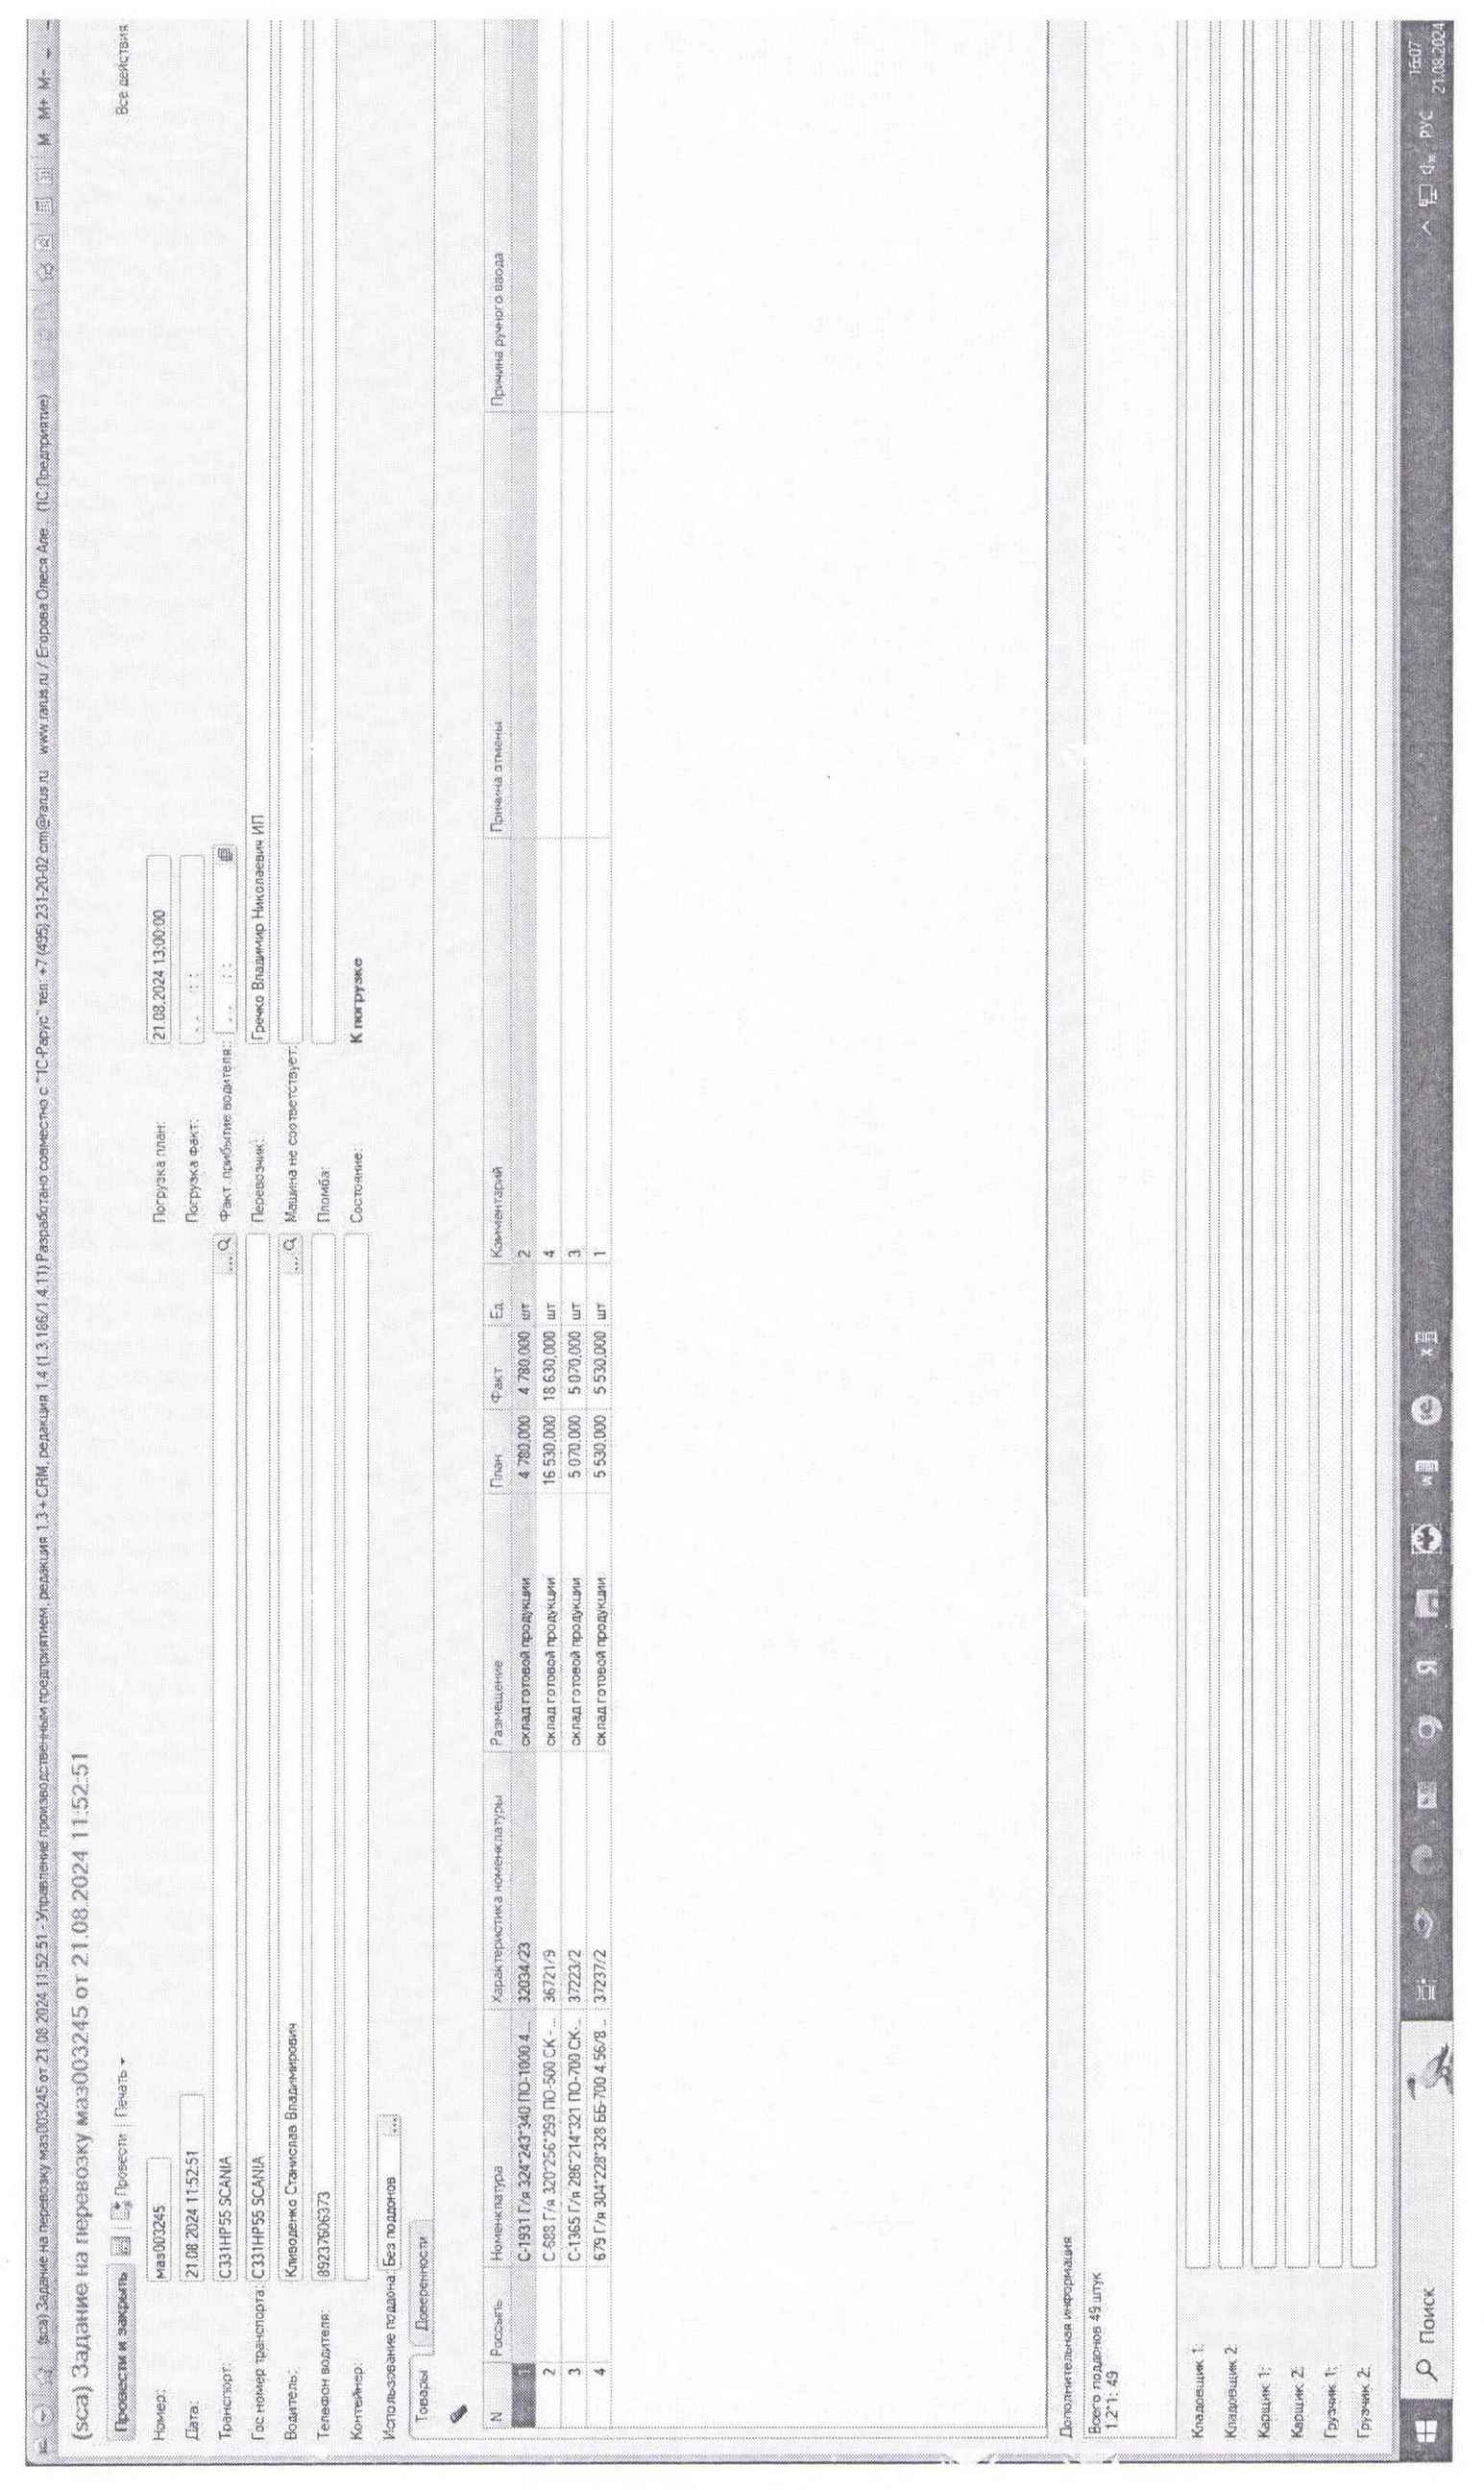
\includegraphics[height=0.8\textheight, width=\textwidth, keepaspectratio]{Pics/d25.jpg}
% \end{center}
%   \caption{План отгрузки готовой продукции}
%   \label{pic:d25}
% \end{figure}

% \begin{figure}
% \begin{center}
%   \includegraphics[height=0.94\textheight, width=\textwidth, keepaspectratio]{Pics/d26_1.jpg}
% \end{center}
%   \caption{Технологическая карта на отгрузку}
%   \label{pic:d26_1}
% \end{figure}

% \begin{figure}
% \begin{center}
%   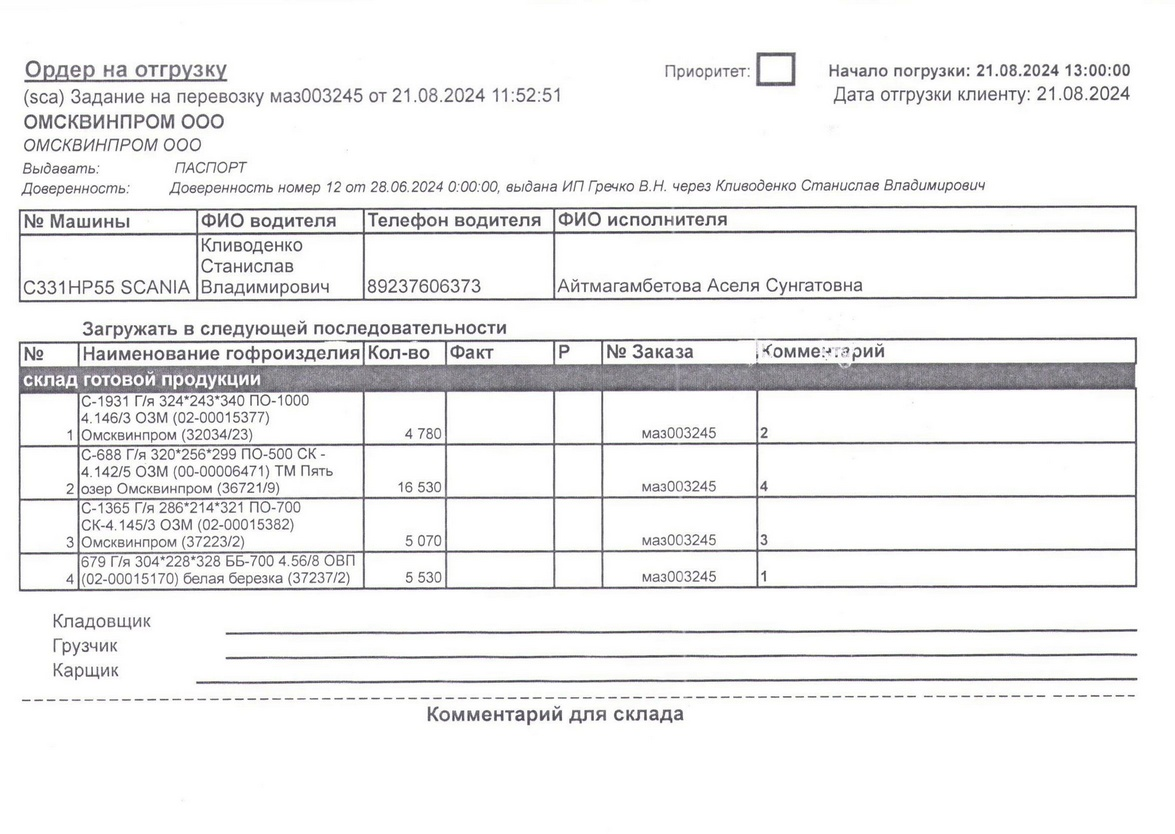
\includegraphics[height=0.94\textheight, width=\textwidth, keepaspectratio]{Pics/d27.jpg}
% \end{center}
%   \caption{Форма заявки на транспорт в СБИС}
%   \label{pic:d27}
% \end{figure}


%Менеджеры отдела продаж контролируют выпуск готовой продукции по появлению остатков ГП. Контроль остатков ведется в файле MS Excel \ref{pic:11_stockGPexcel}. 
%Остатки по ГП актуальны на следующий день после производства к 10:00. 
%Поскольку на предприятии выделены два юридических лица, то менеджеры контролируют остатки по ГП по обеим юридическим лицам. 
%
%Менеджеры отдела продаж ведут файл плана отгрузки \ref{pic:10_shipping_plan1} в электронном виде в формате Excel.
%План отгрузки менеджер формирует на основании заявок на производство \ref{pic:09_OrederToProduction}, где указана желаемая и согласованная дата отгрузки.
%
%План отгрузки в электронном виде находится в сетевом доступе.
%Согласованный план отгрузки менеджер передает логисту для планирования транспорта.
%
%Логист постоянно контролирует файл плана отгрузки \ref{pic:10_shipping_plan1}, определяет на основании плана отгрузки транспорт и формирует план отгрузки с учетом поставки транспорта \ref{pic:10_shipping_plan2}. 
%Логист корректирует планы отгрузки \ref{pic:10_shipping_plan2}, указывает транспортное средство и время прибытия, адреса доставки.
%На предприятии существует собственный транспорт. В сутки собственный транспорт делает от 4 до 10 поездок.
%Согласованный логистом план отгрузки передается на склад в электронном виде через сетевой каталог.
%
%На основании плана отгрузки \ref{pic:10_shipping_plan2} логист формирует заявки сторонним экспедиторам на поставку транспорта \ref{pic:12_application_for_forwarder}, которые отправляются по электронной почте. Логист должен заказать автотранспорт за один-два дня до отгрузки.
%
%Выделены отгрузка авто и жд транспортом (контейнеры). В месяц формируется до 8 контейнеров с ГП. При контейнерной отгрузке  логист должен заказывать у логистической компании контейнер за 10 дней до отгрузки. 
%
%
%
%Менеджер контролирует отгрузку в программе 1С по отчету по продажам либо по журналу реализации. Менеджер корректирует планы отгрузки по факту отгрузки.
%
%
\begin{figure}
\begin{center}
 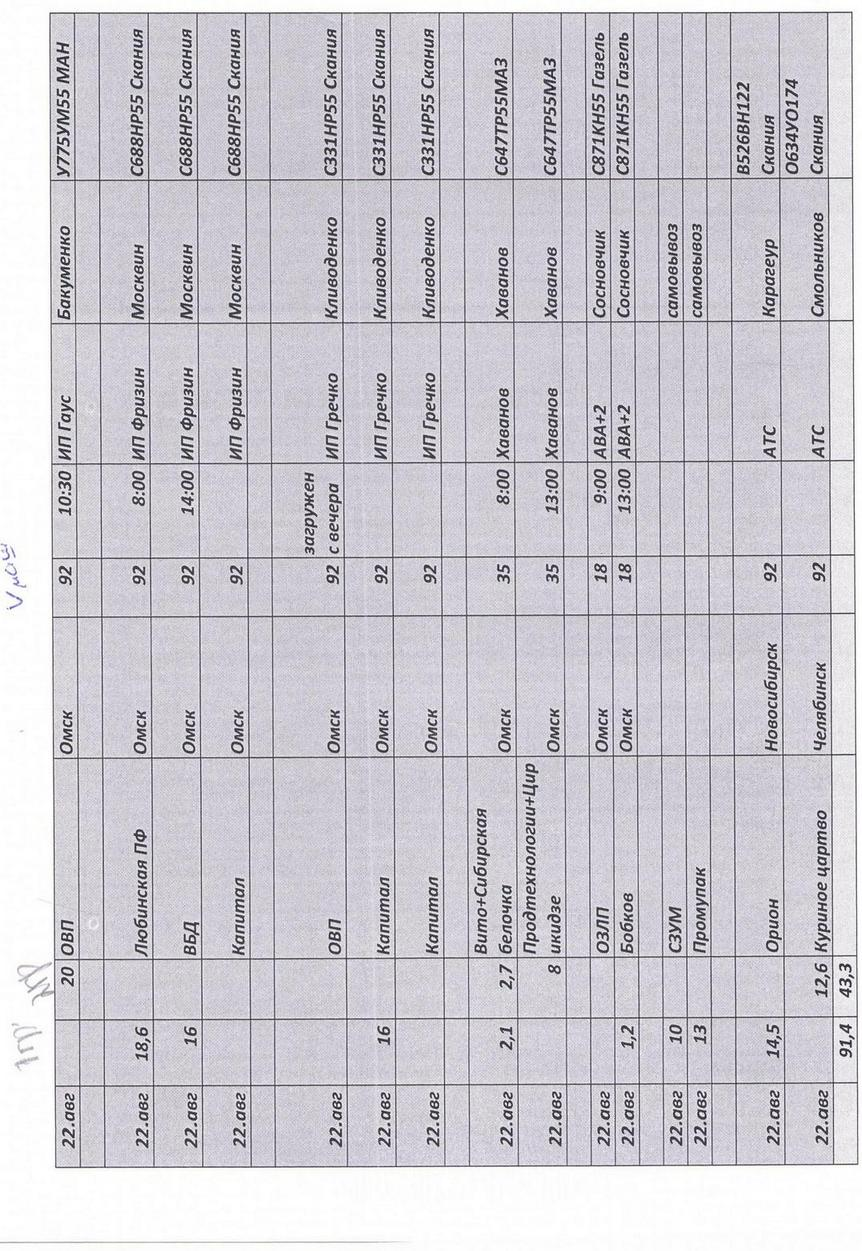
\includegraphics[width=\linewidth, height=0.94\textheight, keepaspectratio]{Pics/d34.jpg}
\end{center}
 \caption{План отгрузки}
 \label{pic:d34}
\end{figure}

\begin{figure}
\begin{center}
 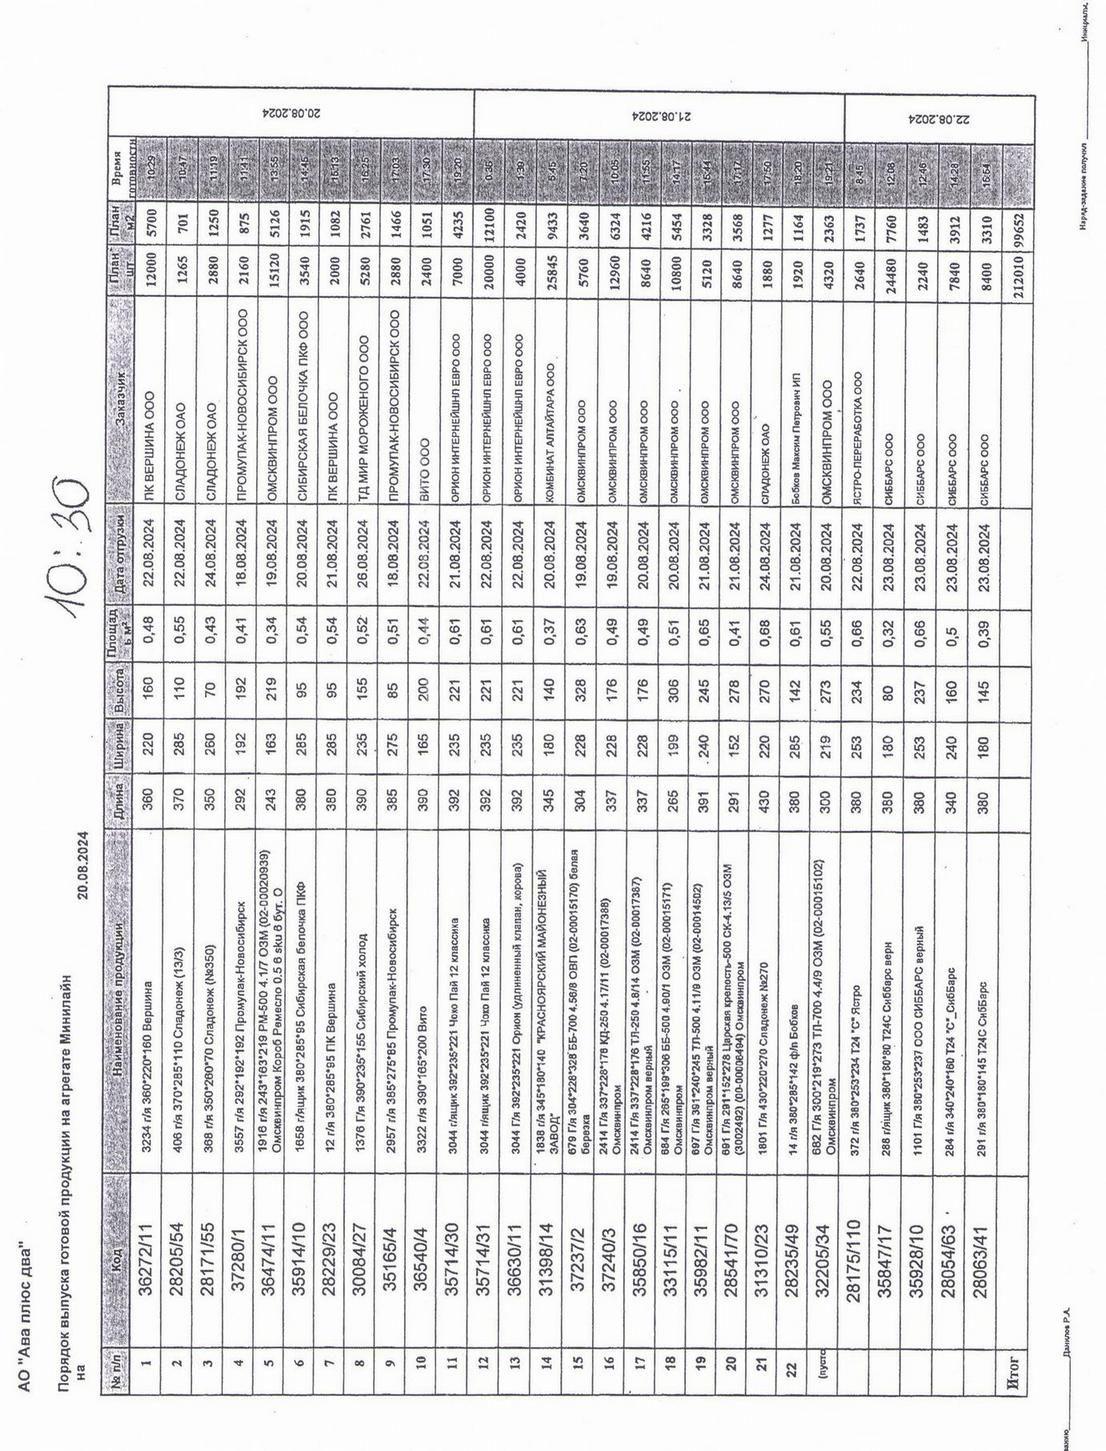
\includegraphics[width=\linewidth, height=0.94\textheight, keepaspectratio]{Pics/d12_2.jpg}
\end{center}
 \caption{Задание на гофроагрегат, экземпляр для менеджеров}
 \label{pic:d12}
\end{figure}

\begin{figure}
\begin{center}
 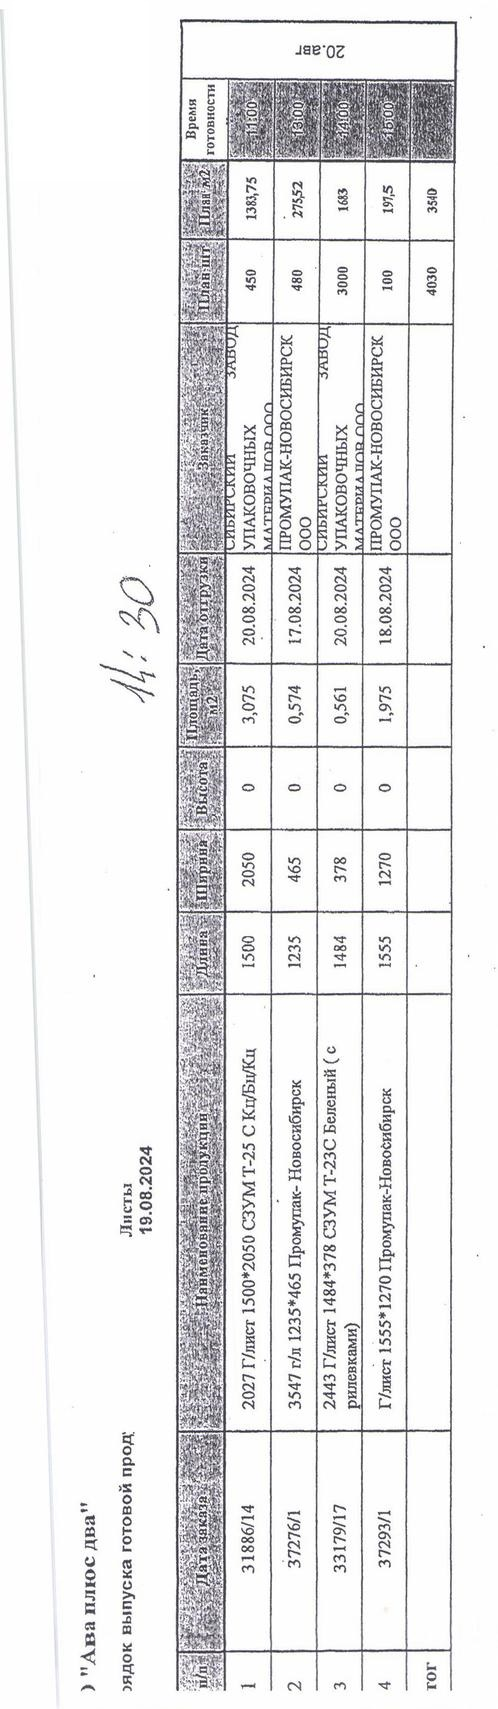
\includegraphics[width=\linewidth, height=0.94\textheight, keepaspectratio]{Pics/d13.jpg}
\end{center}
 \caption{Задание на линии переработки, экземпляр для менеджеров}
 \label{pic:d13}
\end{figure}


\begin{figure}
\begin{center}
 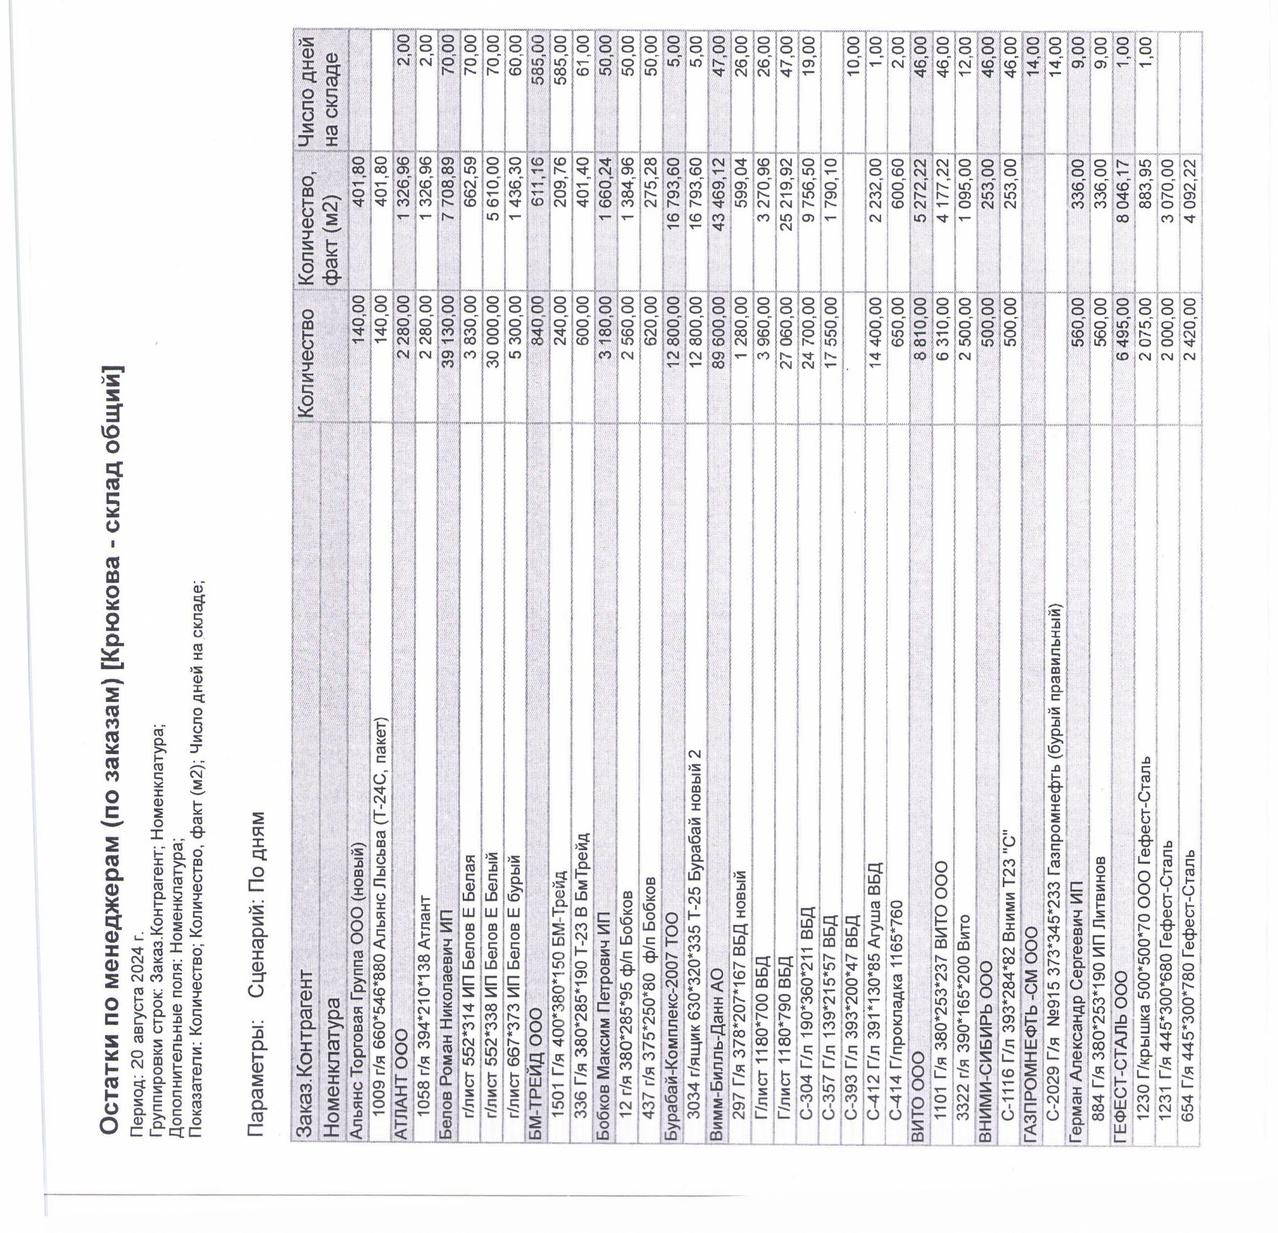
\includegraphics[width=\linewidth, height=0.94\textheight, keepaspectratio]{Pics/d14.jpg}
\end{center}
 \caption{Форма остатков готовой продукции для менеджеров}
 \label{pic:d14}
\end{figure}

\begin{figure}
\begin{center}
 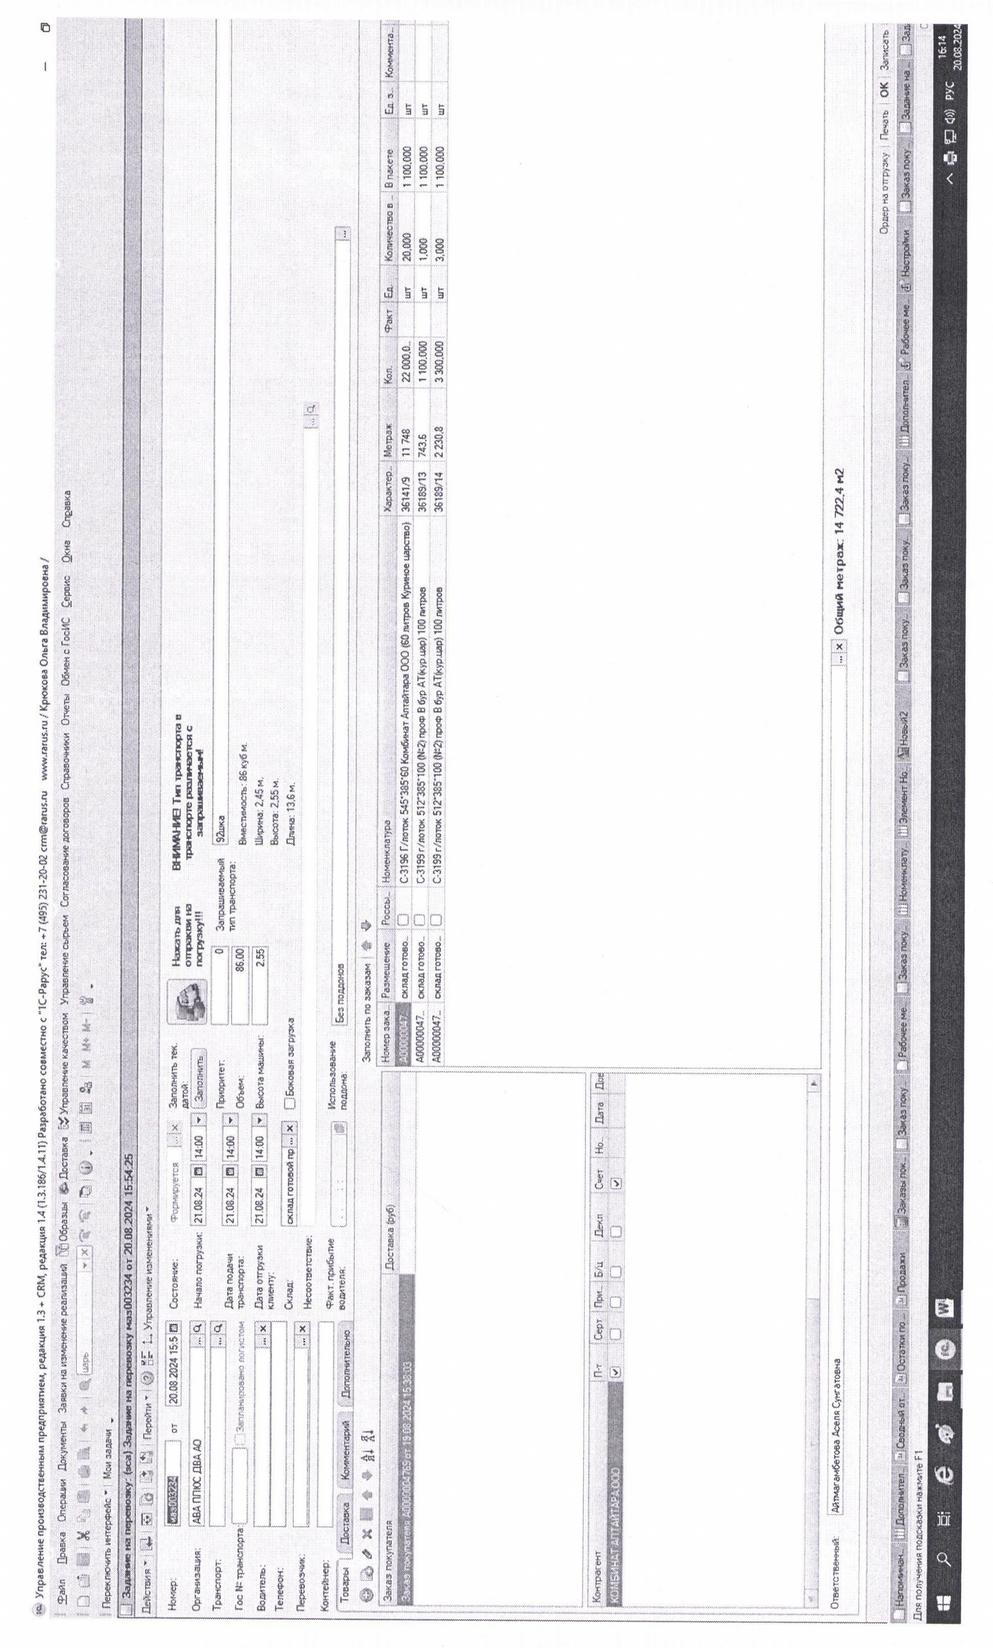
\includegraphics[width=\linewidth, height=0.94\textheight, keepaspectratio]{Pics/d15.jpg}
\end{center}
 \caption{Форма заявки на отгрузку в 1С:УПП}
 \label{pic:d15}
\end{figure}

\begin{figure}
\begin{center}
 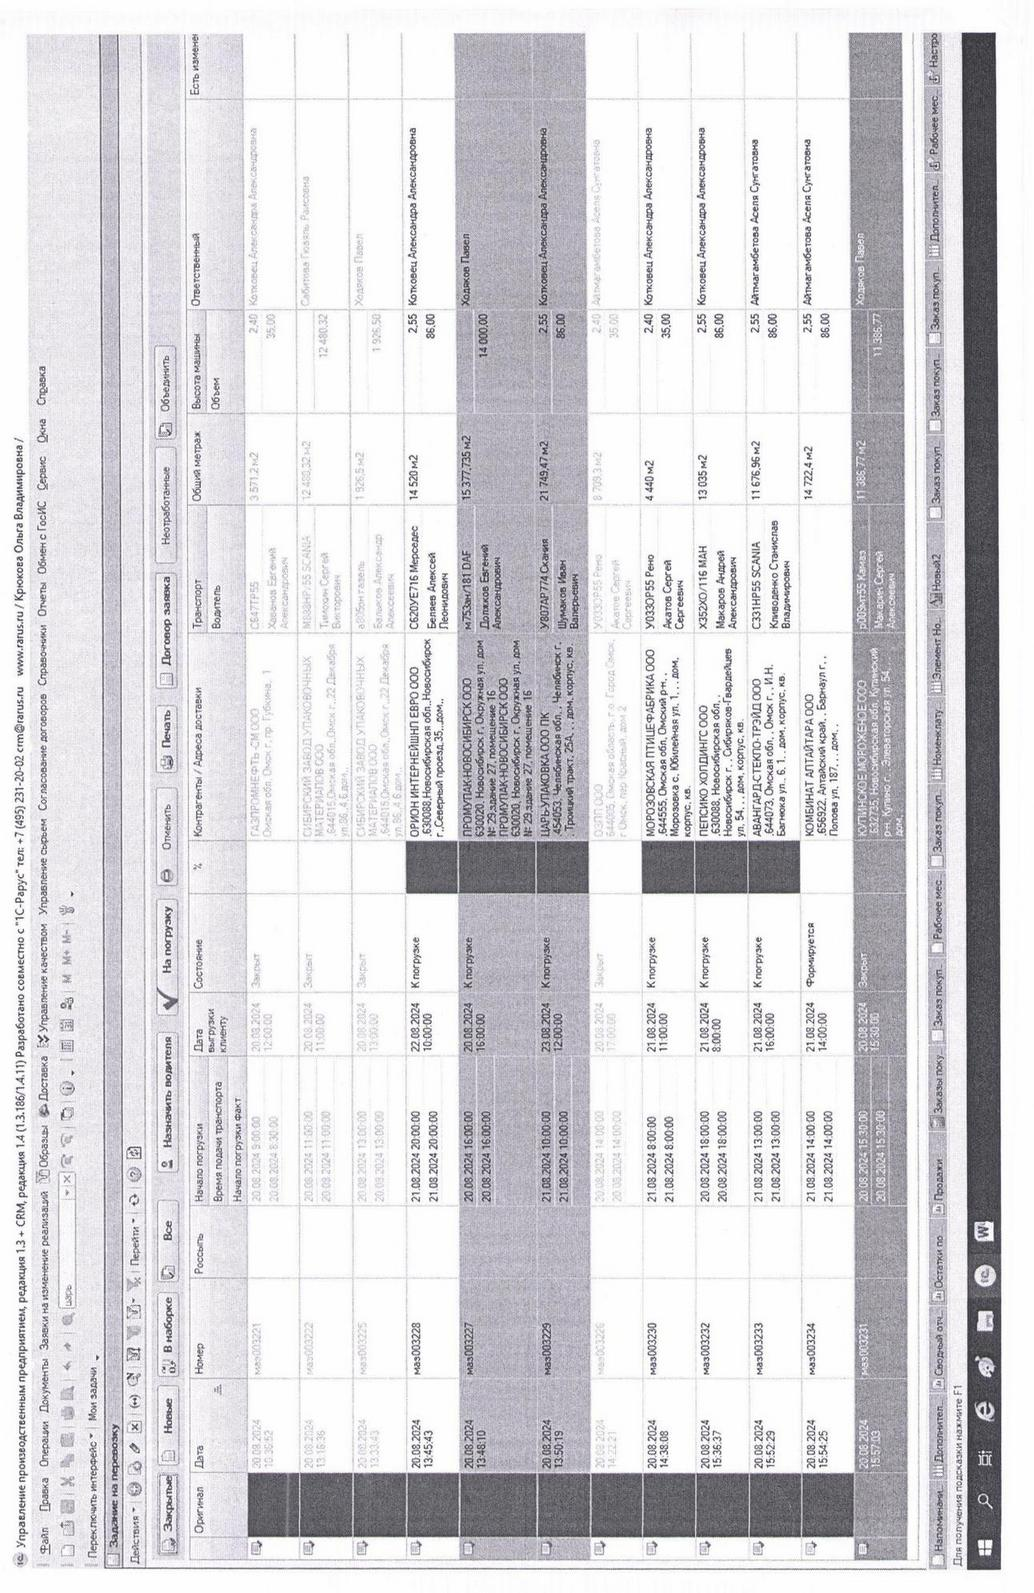
\includegraphics[width=\linewidth, height=0.94\textheight, keepaspectratio]{Pics/d16.jpg}
\end{center}
 \caption{Форма плана отгрузки в 1С:УПП}
 \label{pic:d16}
\end{figure}
\newpage
\subsection{Отгрузка готовой продукции}
\label{bp:Shipment}

Логист передает план отгрузки на склад кладовщику. 

От логиста и менеджера на склад поступает  задание на отгрузку в системе 1С:УПП (форма \ref{pic:d25}, 
% \ref{pic:d26}, 
\ref{pic:d27}).
В форме \ref{pic:d27} указано время подачи машины.

Водитель погрузчика в ТСД выбирает пункт “Отгрузка” и сканирует каждый паллет с готовой продукцией на отгрузку.
Кладовщик указывает  водителю погрузчика, где находятся паллеты с необходимой готовой продукцией согласно задания на отгрузку.
Кладовщик проверяет с заданием и факт отгрузки у водителя в ТСД.
Проверки в ТСД по номенклатуре нет.

Кладовщик по некоторым клиентам ведет журнал остатков по форме \ref{pic:d28}.
Кладовщик дублирует ярлыки на паллеты с более крупным шрифтом для поиска ГП.
Кладовщик информацию по отгрузке дублирует вручную в журнал форма \ref{pic:d29}.

В системе 1С:УПП учет отгрузки организован в разрезе номенклатуры, не по номерам паллет. 
Проверка неверного считывания штрих-кода на ТСД не реализована.

После загрузки машины кладовщик указывает время окончания погрузки в системе 1С:УПП и завершает отрузку.

Одновременно может грузиться 2 машины на пандусах и одна с боковой загрузкой.

У каждого водителя погрузчика есть свой ТСД.
Если готовая продукция под погрузку не помещается в транспорт, водитель погрузчика грузит по порядку, указанному в распоряжении на отгрузку.

При неполной погрузке транспорта водитель погрузчика сообщает через кладовщика менеджеру, что необходимо дополнить транспорт продукцией.


Кладовщики в системе 1С:УПП создает на основании распоряжения на отгрузку документ "Расходная накладная". Строки документа будут скопированы автоматически. Кладовщик из системы 1С:УПП печатает сопроводительные документы: ТН, ТТН, паспорт качества. 

Копии отгрузочных документов кладовщик передает в бухгалтерию.

С распоряжением на отгрузку и пакетом сопроводительных документов водитель выезжает со склада готовой продукции.
Распоряжение водитель отмечает на охране и оставляет. Каждое утро кладовщик передает в бухгалтерию предприятия документы по отгрузке за прошедший день для  сверки факта отгрузки. 

Бухгалтер создает копии отгрузочных документов на основании расходной накладной бухгалтерские документы в системе 1С:Бухгалтерия.




\begin{figure}
\begin{center}
  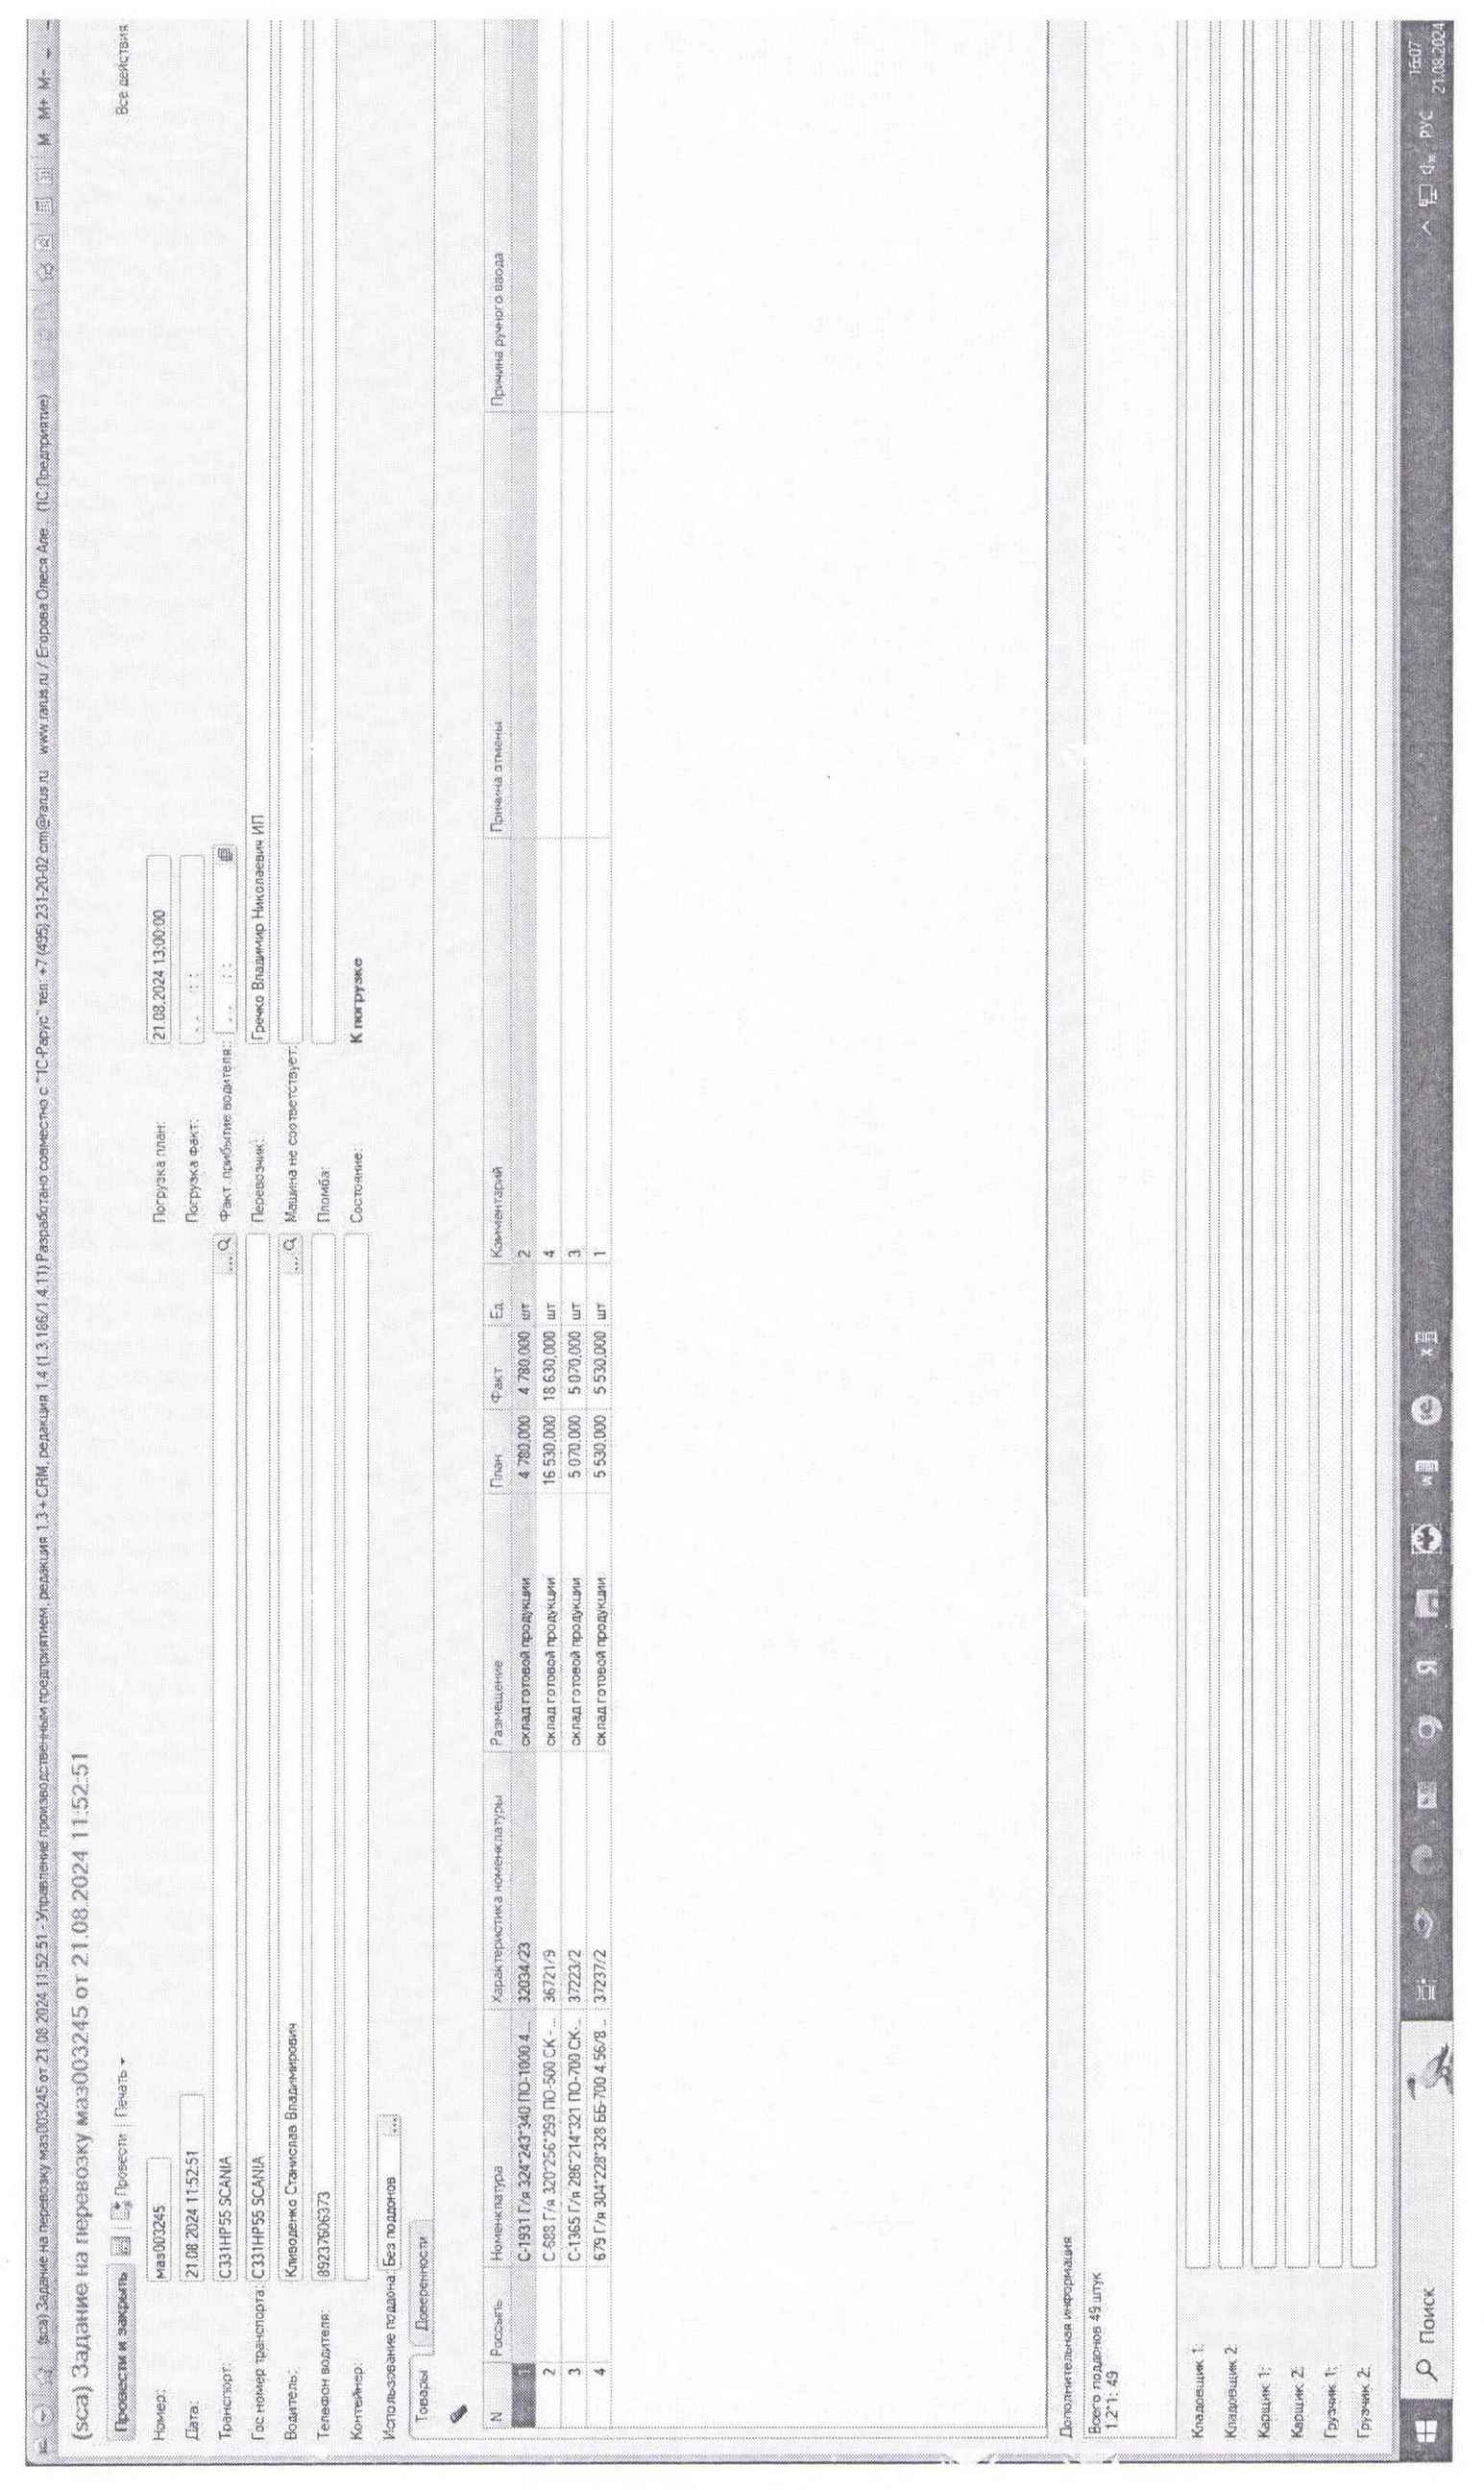
\includegraphics[height=0.8\textheight, width=0.8\textwidth, keepaspectratio]{Pics/d25.jpg}
\end{center}
  \caption{Задание на отгрузку в системе 1С:УПП}
  \label{pic:d25}
\end{figure}



\begin{figure}
\begin{center}
  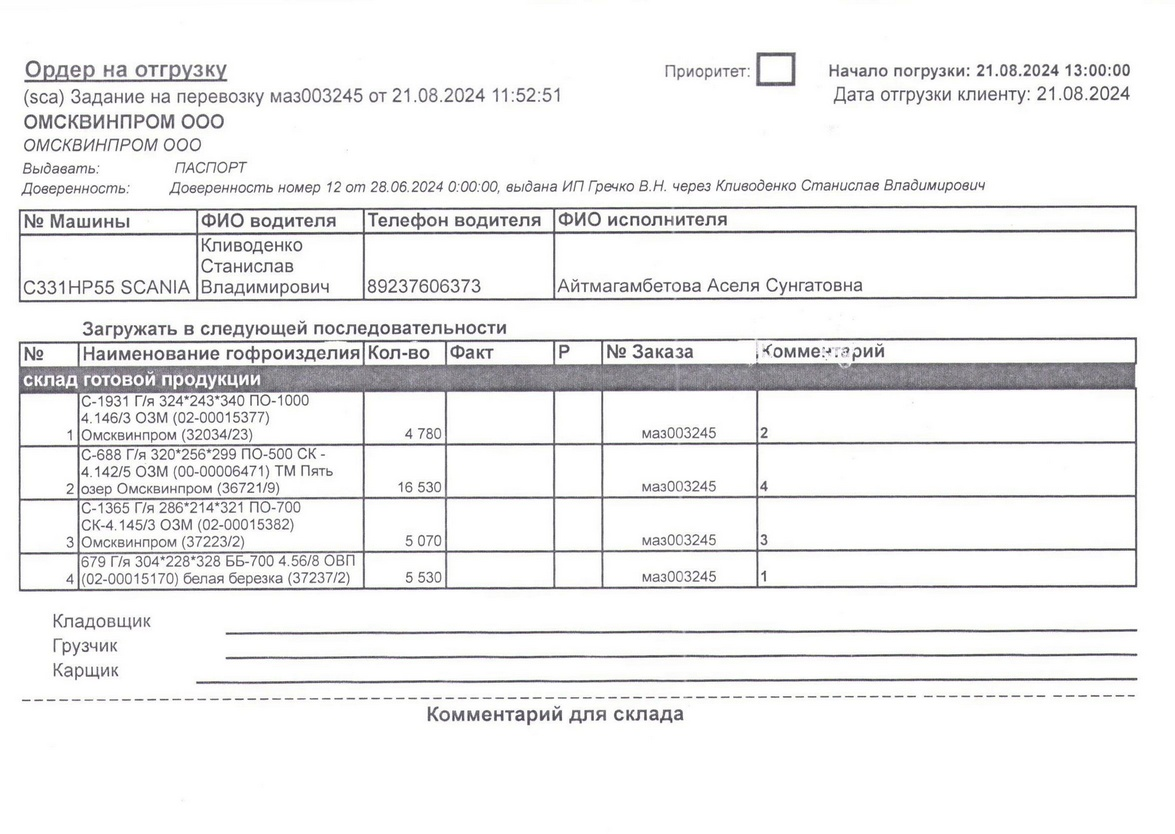
\includegraphics[height=0.6\textheight, angle=90, keepaspectratio]{Pics/d27.jpg}
\end{center}
  \caption{Печатная форма ордера на отгрузку}
  \label{pic:d27}
\end{figure}

\begin{figure}
\begin{center}
  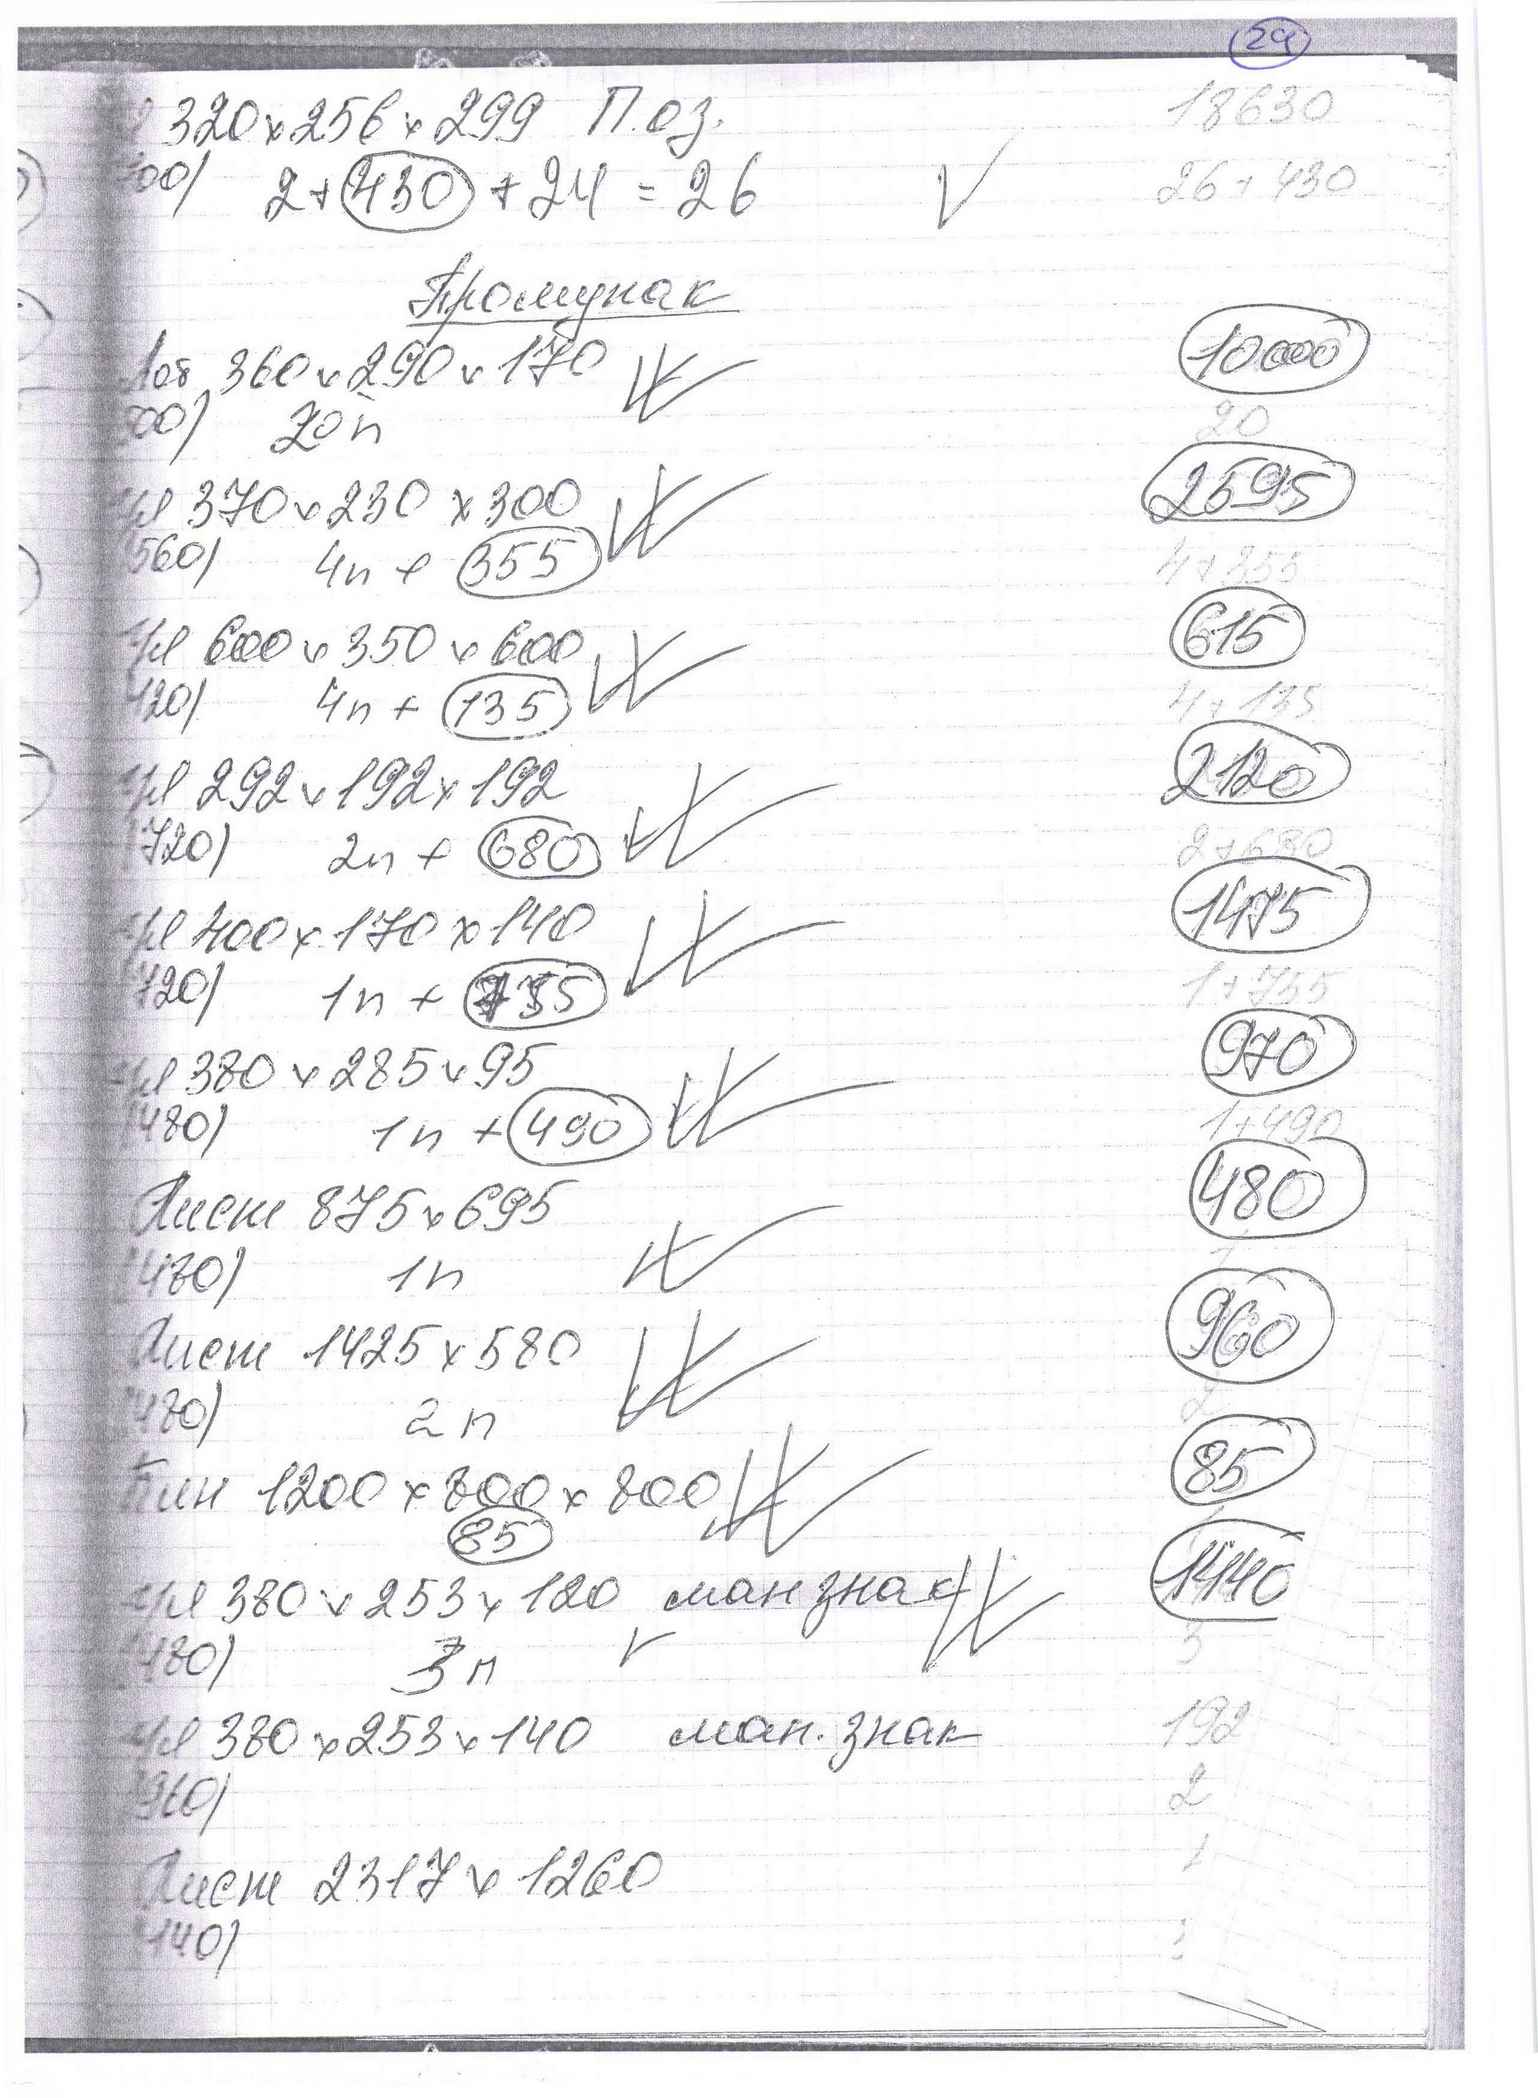
\includegraphics[height=0.8\textheight, keepaspectratio]{Pics/d28.jpg}
\end{center}
  \caption{Журнал остатков по готовой продукции}
  \label{pic:d28}
\end{figure}


\begin{figure}
\begin{center}
  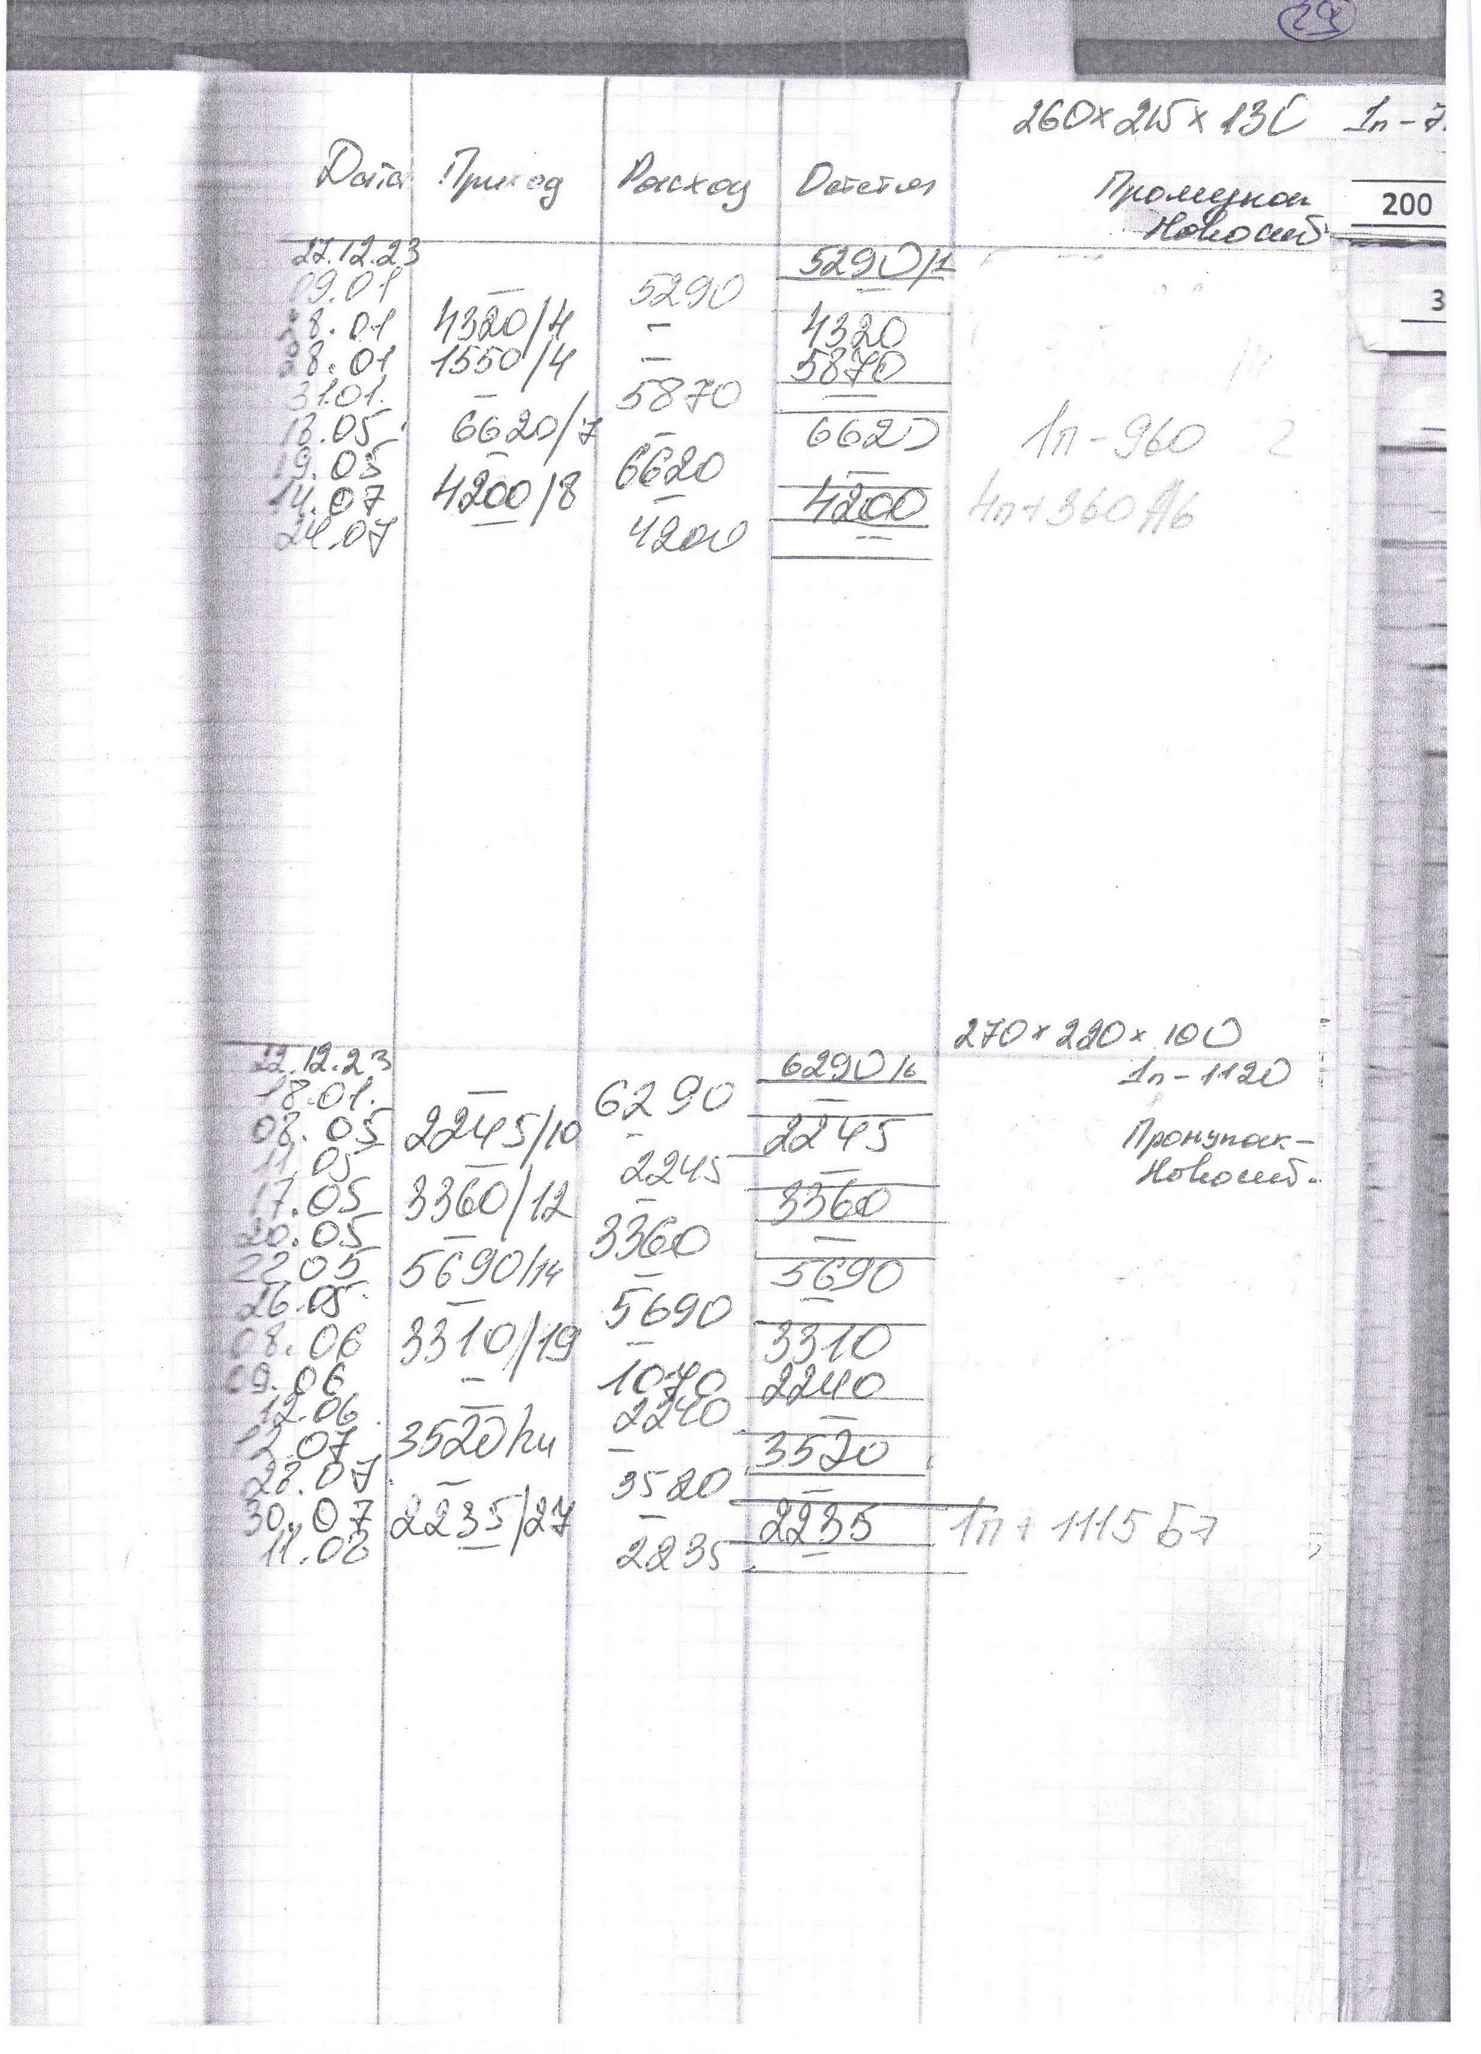
\includegraphics[height=0.8\textheight, keepaspectratio]{Pics/d29_2.jpg}
\end{center}
  \caption{Журнал отгрузки по готовой продукции}
  \label{pic:d29}
\end{figure}

\begin{figure}
\begin{center}
  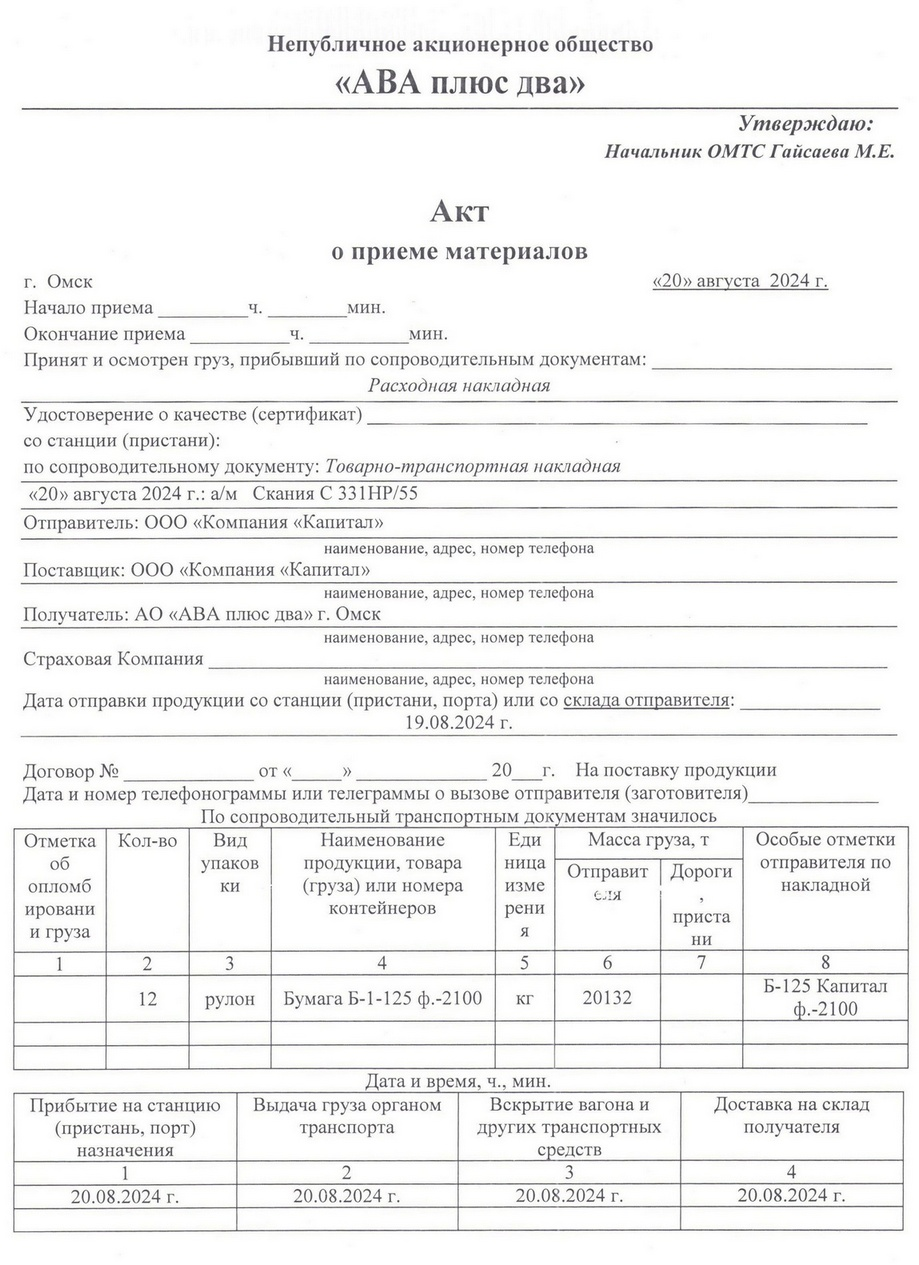
\includegraphics[height=0.8\textheight, keepaspectratio]{Pics/d33.jpg}
\end{center}
  \caption{Акт по приемке материалов}
  \label{pic:d33}
\end{figure}




% Графика подачи машин не выявлено. Машины на погрузку подъезжают в порядке очереди.
% По факту поступления машины кладовщик принимает машину. 
% Кладовщик грузит готовую продукцию по факту на основании плана погрузки и заявки из 1С. Остатки могут остаться на складе. 
% Кладовщик отмечает в заявке покупателя факт отгрузки, передает в отдел учета.

% Кладовщик по отгрузке или мастер смены ночью пишет накладную (рис. \ref{pic:d17}).
% Машина ночью грузится, но ее не отпускают.
% Кладовщик на площадке 1 пишет накладную (рис. \ref{pic:d18}), сканирует и высылает в отдел складской логистики. 
%  По второй площадке Кладовщики пишут заявку покупателя. 
% % (рис. \ref{pic:d19}).
% Кладовщик сам печатает другие бирки на складе по готовой продукции, меняет дату, клиента (рис. \ref{pic:d40}).

% В Google Tab Кладовщики меняет списание по факту.
% Существуют заявки от менеджеров, где указывается количество листов по готовой продукции (рис. \ref{pic:d41}).
% Менеджер может попросить отгрузить другое количество, чем указано в упаковке на паллете (рис. \ref{pic:d42}). Кладовщик может разукомплектовать чужой паллет при необходимости. При этом перепечатывает бирку.

 
% Кладовщик пишет накладную (рис. \ref{pic:d43}), сканирует, отправляет оператору по емайл. Оператор 1С создает в системе 1С: Бухгалтерия накладную, печатает сопроводительные документы, передает водителю.


% Отдел складской логистики на основании накладных (рис. \ref{pic:d17}, \ref{pic:d18})
% % или \ref{pic:d19}) 
% выписывает расходную накладную в системе 1С: Бухгалтерия (упр) и в реальной 1С: Бухгалтерия по юридическому лицу, указанному в заявке.
% В заявке на поставку указано юридическое лицо, от которого будет реализация.
% Отдел логистики печатает расходную накладную и при необходимости пакет сопроводительных документов.

% Паспорта качества по готовой продукции не печатаются.

% В течение дня 
% % по форме \ref{pic:d19}
% оператор 1С создает документ ''Отчет производства за смену''. На основании документа ''Реализация'' учетчик создает в системе 1С Бухгалтерия документ ''Перемещение'' с производства на склад и документ ''Реализация'' по факту отгрузки.

% По площадке 1 учетчик получает заявку на отгрузку. В системе 1С Бухгалтерия создает документ ''Поступление ТМЦ'', ''Перемещение'' и ''Реализация''. Форму накладной отсылает почтой на склад.
% Учетчик регистрирует поступление готовой продукции только в системе 1С Бухгалтерия (Упр). В информационной базе 1С по 
% ИМ Макаров учетчик создает только документ ''Реализация''. В информационной базе 1С по фирме  Норд-Пак учетчик создает документ ''Отчет производства за смену'' и документ ''Реализация''.




% \begin{figure}
% \begin{center}
%   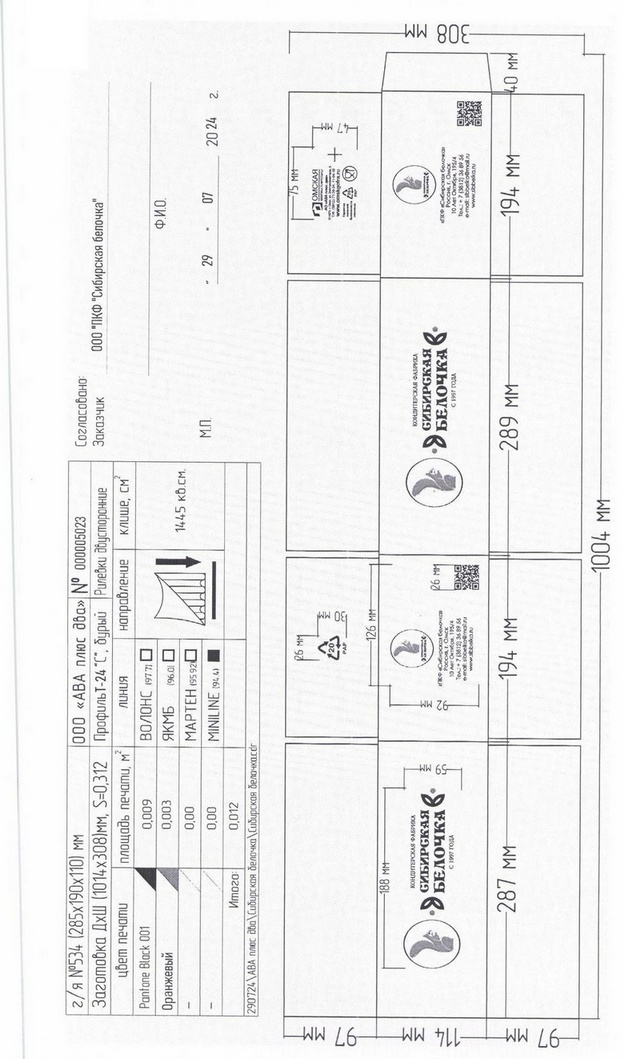
\includegraphics[height=0.94\textheight, keepaspectratio]{Pics/d17.jpg}
% \end{center}
%   \caption{Накладная на отгрузку готовой продукции площадка 3}
%   \label{pic:d17}
% \end{figure}

% \begin{figure}
% \begin{center}
%   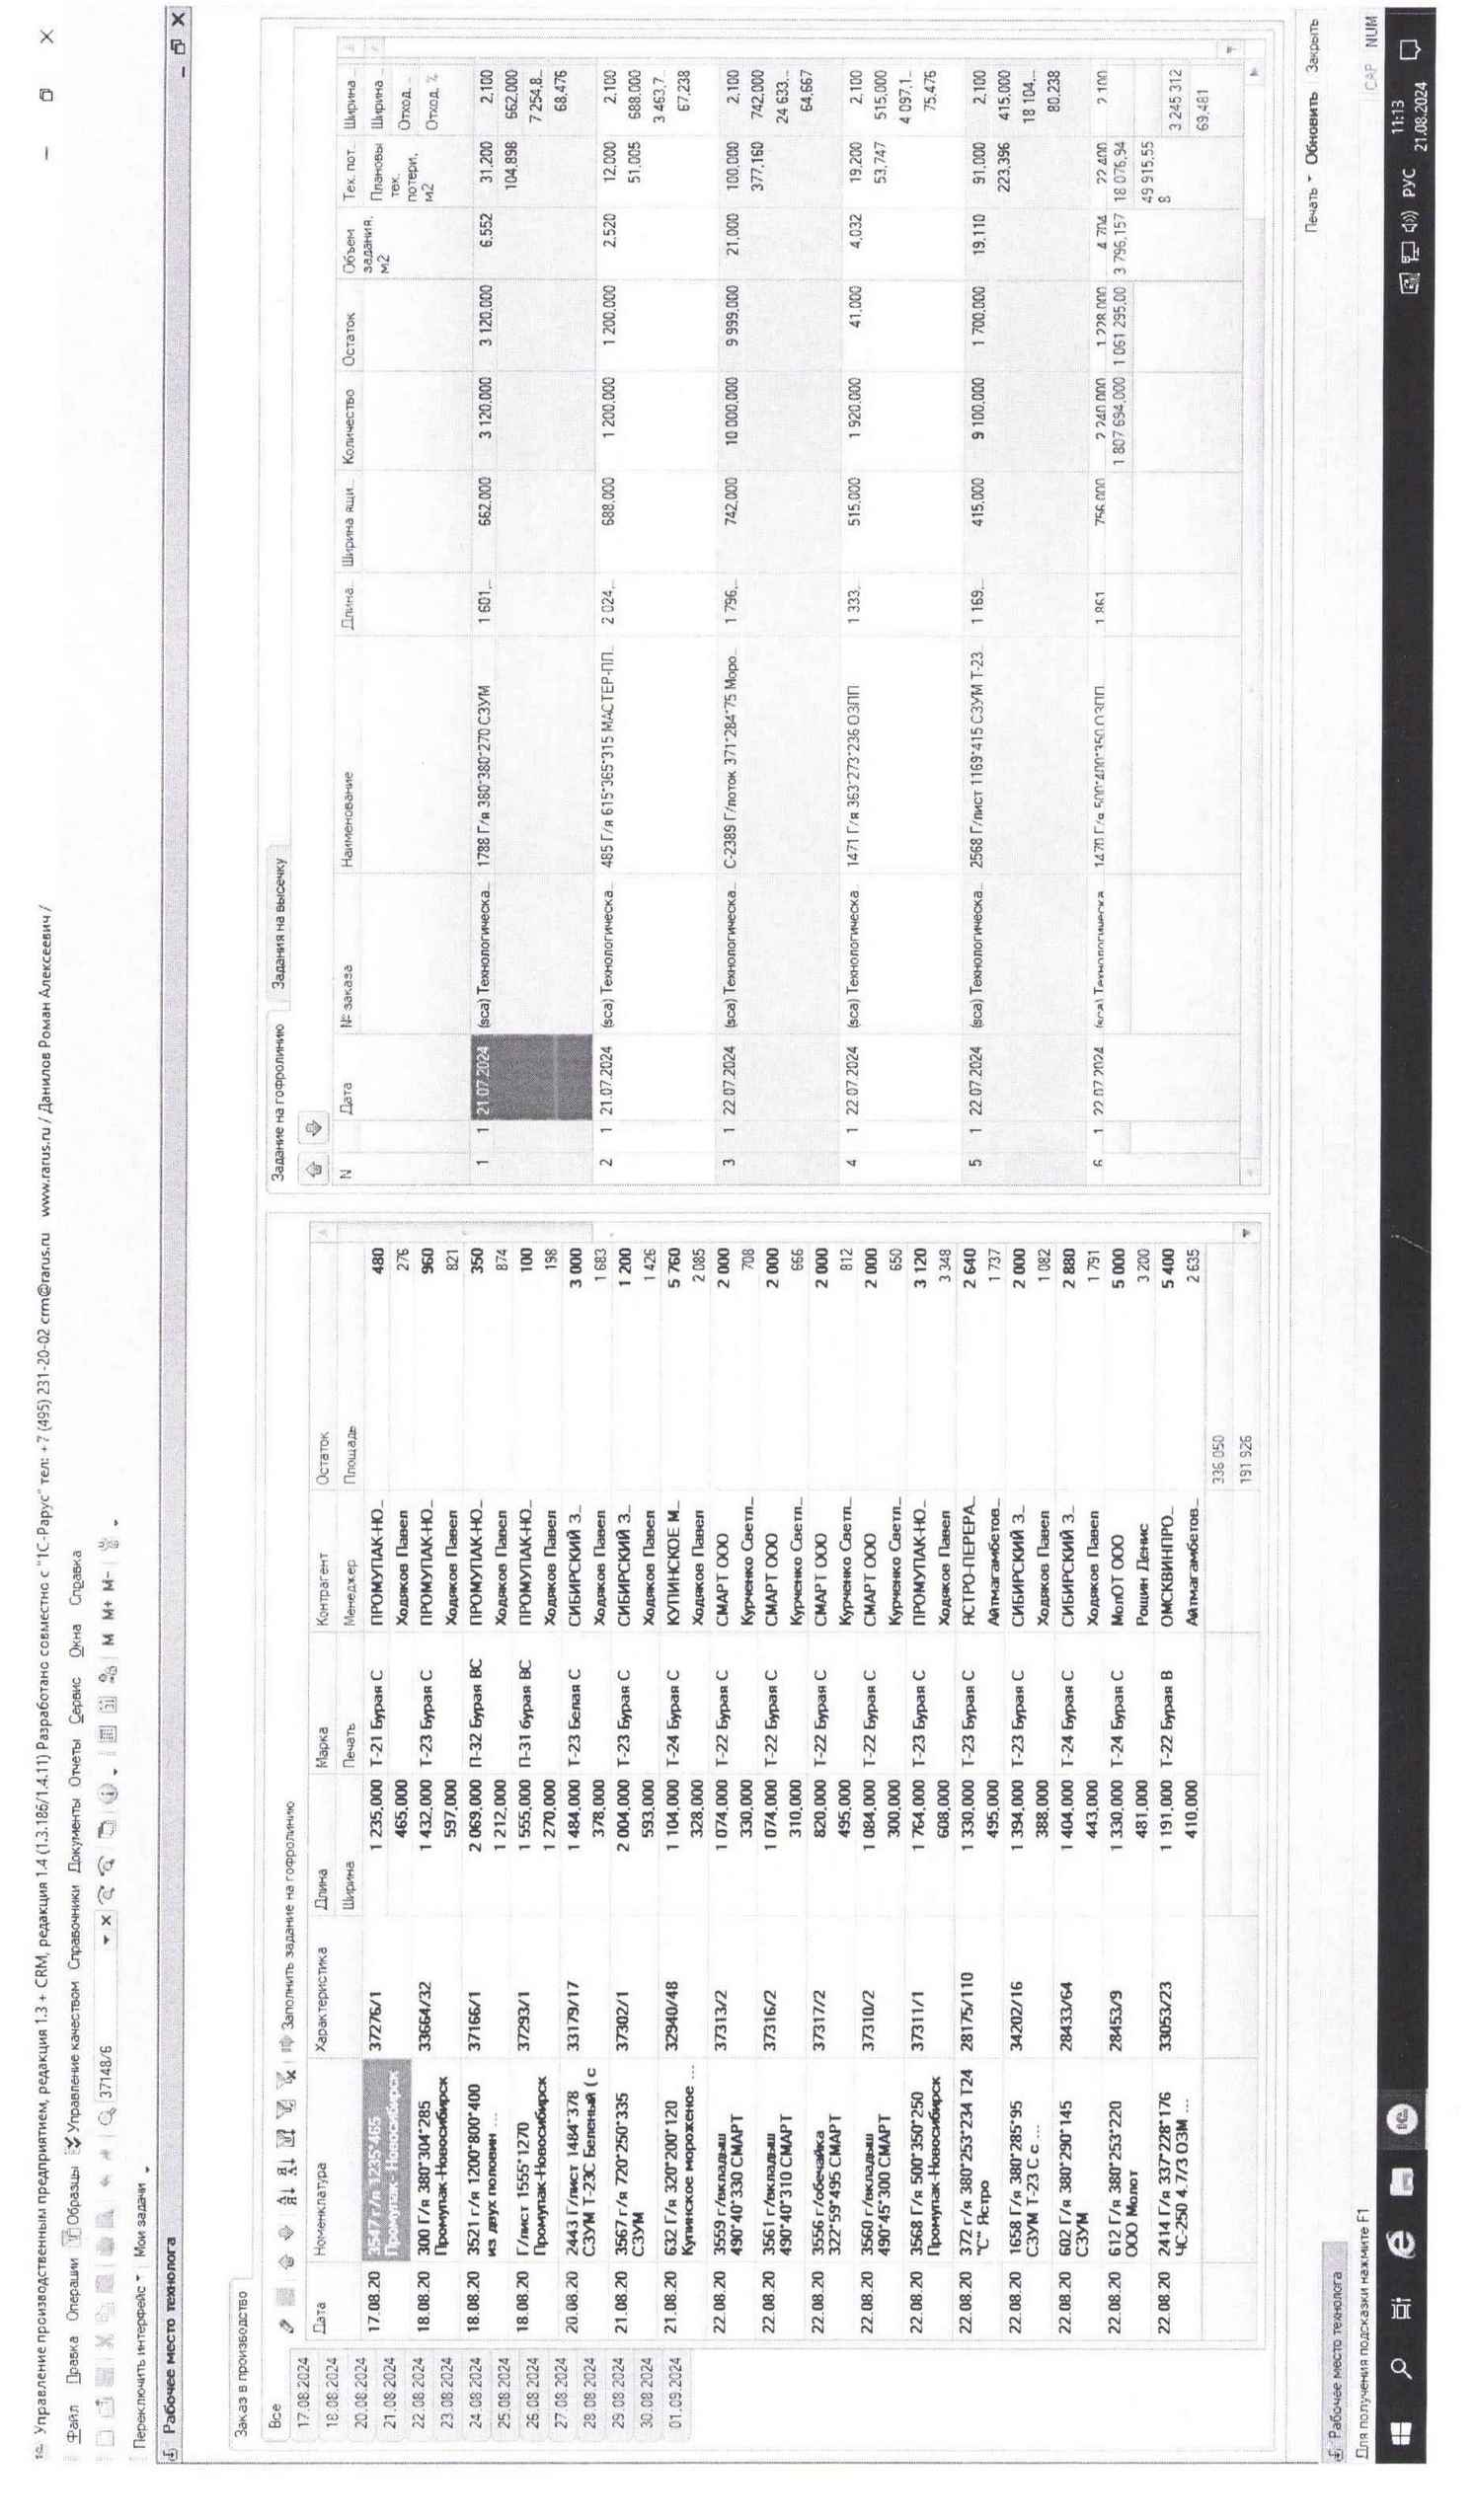
\includegraphics[height=0.94\textheight, keepaspectratio]{Pics/d18.jpg}
% \end{center}
%   \caption{Накладная на отгрузку готовой продукции площадка 1}
%   \label{pic:d18}
% \end{figure}




% \begin{figure}
% \begin{center}
%   \includegraphics[height=0.94\textheight, keepaspectratio]{Pics/d43.jpg}
% \end{center}
%   \caption{Накладная на отгрузку готовой продукции площадка 2}
%   \label{pic:d43}
% \end{figure}

\clearpage
\newpage
\subsection{Планирование сырья}
\label{bp:RawMaterialPlanning}

\textbf{Планирование бумаги и картона}

Планирование основного сырья (бумага и картон) выполняет специалист отдела снабжения.
На гофроагрегате при использовании сырья разработан нормативный документ по возможным заменам сырья. 
Планирование сырья выполняется в конце месяца на будущий месяц.

Специалист отдела снабжения ведет таблицу в Excel (форма \ref{pic:d35}) по планированию сырья.
Для планирования сырья специалист отдела снабжения получает остатки из системы 1С:УПП по форме \ref{pic:d36}.
Товары в пути определяет по данным своего файла форма \ref{pic:d35} вручную.
Специалист отдела снабжения определяет расчетным путем остаток сырья в месяцах работы оборудования.
План закупки специалист отдела снабжения считает вручную в форме \ref{pic:d37}.
Далее специалист отдела снабжения распределяет потребности в сырье по поставщикам. Cпециалист отдела снабжения создает запрос у поставщиков по цене и объемам поставки на каждый месяц.

Специалист отдела снабжения создает вручную заявку на поставку по форме \ref{pic:d38}.

Потребности в краске определяет отдел ОТК (отдел подготовки производства).
Заказывает краску специалист отдела снабжения.
В системе 1С:УПП специалист отдела снабжения смотрит только приход материалов.



% \textbf{Планирование закупки заготовок}

% На производстве выделены популярные позиции заготовок, по которым имеется складской запас. 


% По таким изделиям МСЗ контролируют объем неснижаемого запаса вручную и при необходимости создают заказы покупателя на контрагента ООО ''Рускартон'' (на склад). 
% Остальные заготовки поступают сразу в производство под конкретный производственный заказ.
% МСЗ на основании заказа покупателя создает заказ на бронь по складским свободным остаткам. Остатки МСЗ может узнать по отчету в 1С:УНФ «Остатки ГП». В момент отгрузки менеджер снимает с резерва свободные остатки в разрезе заказа покупателя.

% Планированием закупки заготовок занимается инженер по планированию.
% Заказ от менеджера поступает в системе 1С:УНФ инженеру по планированию, который на основании плана производства в таблице MS Excel (рис. ??) создает в системе 1С:УНФ документ ''Заявка на продажу'' (рис. \ref{pic:d17}). 

% % \todo{перечитать с планированием}

% При создании заказа менеджеры стараются создавать заказ на производство кратно поддону. 
% Инженер по планированию ставит в системе 1С:УНФ у документа ''Заказ на производство'' статус «В работе» и заказывает заготовки у поставщиков согласно заказам на производство. Объем заказа заготовок в точности совпадает с объемом заказа на производство.
% На основании формы \ref{pic:d15} инженер по планированию формирует заявку на производство (заготовки) и заявку на ресурсе поставщика.

\textbf{Планирование вспомогательных материалов}

Планированием и закупкой вспомогательных материалов занимается отдел снабжения.

% Каждый день техник по учету определяет остатки по крахмалу и другим материалам (Пленка, скотч и др.) в производстве и сообщает по телефону в отдел снабжения остатки на складе. 25 числа каждого месяца менеджер по снабжению заказывает поставки крахмала на следующий месяц. Объемы заказа определяются коллективно с техником по учету. Менеджер отдела снабжения обзванивает поставщиков по ценам, формирует заявку в свободной форме. Поставки крахмала выполняются 2-3 раза в месяц.

В системе 1С:УПП хранятся текущие остатки на складах.


По закупке других материалов (СИЗ, спецодежда, комплектующие и запчасти) отдел снабжения собирает заявки от подразделений, обрабатывает их, ищет поставщиков и производит закупку.


\textbf{Поддоны}

Учет поддонов осуществляется в Файле MS Excel, который ведет главный технолог. Но заказ поддонов производят начальники смен. Начальники смен определяют потребность в поддонах исходя из плана производства и текущих остатков на складах и  сообщают в отдел снабжения. Отдел снабжения производит закупку необходимого количества поддонов.  
% Начальник склада каждый вечер определяет потребность по поддонам и сообщает по телефону в отдел снабжения, где менеджеры отдела снабжения фиксирует вручную объемы потребности.
% Коммерческий отдел и отдел снабжения совместно определяют потребность в поддонах исходя из плана производства и текущих остатков на складах и заказывают поддоны у производителей.
% Менеджеры отдела снабжения создают заявку на закупку поддонов и спецподдонов. Все поддоны невозвратные.
% Поддоны принимаются на складе. Учет поступления фиксируется в системе СБИС.


\textbf{Планирование краски}

На предприятии используют готовую краску. Учет краски возложен на контролеров по качеству (технологов). Остатки  краски технолог определяет визуально и сообщает специалисту отдела снабжения позиции, которые необходимо приобрести. Отчеты по расходу ведутся в MS Excel и контролируются главным технологом  \ref{pic:1.9 отчет о расходе сырья и материалов 2_0001}.
%\todo{ПИСАТЬ}
% Краску заказывает техник УВФ (???). Остатки основы и пигментов краски техник определяет визуально и по опыту заказывает необходимый объем напрямую у поставщика.



%Оснастку тоже.

% Закупками краски занимается инженер по планированию. Краска в цеху списывается ежедневно. Инженер по планированию ориентируясь на недельный план в таблице MS Excel, составляет потребность в краске на неделю и сравнивает с остатками в 1С (рис. \ref{pic:a80}). При наличии нужного пантона менее 20 кг (1 ведра), заказывается еще 20 кг.

% \begin{figure}
% \begin{center}
%   \includegraphics[height=0.6\textheight, keepaspectratio]{Pics/a80.jpg}
% \end{center}
%   \caption{Остатки по краске}
%   \label{pic:a80}
% \end{figure}
% \clearpage

% \textbf{Планирование вспомогательных материалов }

% Вспомогательные материалы закупает инженер по планированию. Списание на производстве происходит в конце месяца. По просьбе инженера по планированию кладовщик может пересчитать и предоставить остатки на бумаге (\ref{pic:a57}). Ориентируясь на них инженер по планированию закупает необходимые материалы. Клей закупает на месяц 240 кг (1 бочка).

% Мастер производства заказывает поддоны  по телефону, контролирует остатки  и заказывает недостающее количество. Перемещение поддонов выполняет  бухгалтер по накладной (\ref{pic:a31}). Поддоны от поставщиков (приходит заготовка) сразу увозят на другую площадку для сортировки. 

\begin{figure}
\begin{center}
  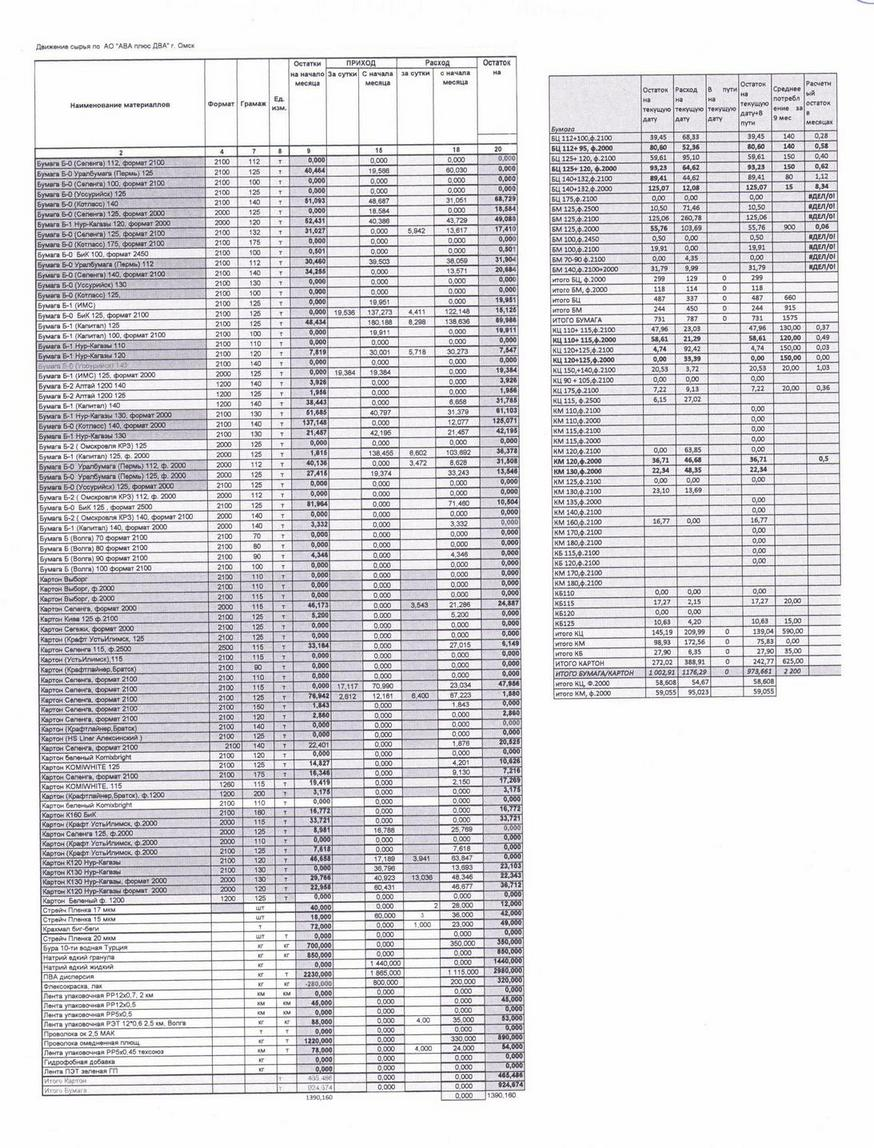
\includegraphics[height=0.9\textheight, keepaspectratio]{Pics/d35.jpg}
\end{center}
  \caption{Форма планирования сырья}
  \label{pic:d35}
\end{figure}
\clearpage

\begin{figure}
\begin{center}
  \includegraphics[height=0.8\textheight, keepaspectratio]{Pics/d36.jpg}
\end{center}
  \caption{Форма остатков из системы 1С:УПП по бумаге и картону}
  \label{pic:d36}
\end{figure}
\clearpage

\begin{figure}
\begin{center}
  \includegraphics[height=0.8\textheight, keepaspectratio]{Pics/d37.jpg}
\end{center}
  \caption{Форма расчета потребности в сырье}
  \label{pic:d37}
\end{figure}
\clearpage

\begin{figure}
\begin{center}
  \includegraphics[height=0.8\textheight, keepaspectratio]{Pics/d38.jpg}
\end{center}
  \caption{Форма заявки на поставку сырья}
  \label{pic:d38}
\end{figure}
\clearpage

\begin{figure}
\begin{center}
  \includegraphics[height=0.6\textheight, angle=90, keepaspectratio]{Pics 1/1.9 отчет о расходе сырья и материалов 2_0001.jpg}
\end{center}
  \caption{Учет сырья и материалов в MS Excel}
  \label{pic:1.9 отчет о расходе сырья и материалов 2_0001}
\end{figure}
\clearpage
%
\clearpage
\ifx \notincludehead\undefined
\normalsize
\end{document}
\fi
%\newpage
\subsection{Оперативное планирование производства}
\label{bp:OperPlan}

Все заявки от покупателей  менеджеры отдела продаж регистрируют в системе 1C:УПП (рис. \ref{pic:2.1 Заказы в УПП_0001}). 

%Менеджер выгружает в отдел планирования в системе СБИС заявки покупателей. 
Специалист по планированию производства (ПП) производит перенос заказов из 1C:УПП в документ MS Excel "AVA заказы" (рис. \ref{pic:2.1 Заказы в файле эксель АВА_0001}). Специалист ПП производит перенос заказов несколько раз в течение рабочего дня. Регламент приема заказов отсутствует. Задача --- набрать объем заказов для обеспечения загрузки производства. Специалист ПП ориентируется на желаемую дату производства, которую указал менеджер. Возможно срочное добавление заказов. Заказы, которые последними перенесены из системы  1С: УПП, вставляются в конец списка. По каждому заказу  ориентируясь на ТК и свой опыт  специалист ПП указывает маршрут для производства. Специалист ПП переносит заказы на вкладку "Каталог заказов". По каждому заказу в ручную переносятся данные по размерам заготовок, марке и профилю (рис. \ref{pic:2.4 каталог заказов_0001}). 
На предприятии организовано планирование от линий переработки. 

\textbf{Планирование линий переработки}

Для  планирования ручных и автоматических линий переработки специалист ПП переходит в файл MS Excel "Драм" (рис. \ref{pic:2.6 Задание на ручной станок в Драм_0001}). Задания на ручные линии переработки указывается без расчета времени на выработку заказа. На автоматические линии расчет времени производится исходя из плановой производительности  без учета сложности изготовления (рис. \ref{pic:2.6 задание на линию в Драм_0001}). Плановая производительность устанавливается генеральным директором (рис. \ref{pic:4 План выработки в шт}). Время переналадки и технологические перерывы не учитываются. Время начала работы каждой линии переработки указывается. 
Специалист ПП печатает задания на сетевой принтер, установленный на производстве у начальника смены, в 15-30 на вечернюю смену и следующую смену.

Каждое утро рабочего дня специалист ПП формирует в системе 1С:УПП отчет по выработке продукции (рис. \ref{pic:0 Отчет выпуск продукции и услуг_0001}) и сравнивает данные с файлом MS Excel "Драм". В файле  "Драм" в ручную переносятся данные о выработке заказов. Если отклонение от выпуска по заказу превышает 5 процентов, то специалист ПП совместно с менеджером принимает решение --- считать заказ выработанным или нет. Если отклонение менее 5 процентов, то специалист ПП самостоятельно удаляет заказ из очереди. 

\textbf{Планирование выпуска на гофроагрегате}

На каждый заказ производства менеджер создает новую характеристику номенклатуры в системе 1С:УПП копированием ТК. Таким образом планирование выполняется не по заказам, а по коду характеристики в системе 1С:УПП.


Планирование и создание заданий  на выпуск продукции и заготовок на гофроагрегате производится в файле MS Excel ''Драм'' (рис. \ref{pic:0 Крой в эксель_0001}). Основные форматы, используемые при крое: 2000 мм, 2100 мм, 2500 мм. Дополнительно может быть использован формат 2450 мм. Выпускаемые профили гофры: В,С,Е,ВС, ВЕ. Максимальное количество полос для кроя --- 6 полос. Планирование гофроагрегата ведется от загруженности линий переработки с учетом типов выпускаемых изделий. Планирование осуществляется только на смену с 8-00 до 20-00. План выпуска на смену установлен 138600 м2. Допустимая кромка отхода по полотну составляет 3\%. Количество раскроев на смену в среднем составляет более 20.

Из документа MS Excel "АВА заказ" специалист ПП вручную переносит размеры заготовок по каждому заказу. Исходя из своего опыта специалист ПП собирает вручную "блоки" по форматам, профилям и маркам.  Специалист ПП вручную производит поиск подкроя для каждого заказа, ориентируясь на значение кромки. Рилевки проверяются также вручную. Часто возникают проблемы с поиском подкроя к заказам на профилях: ВС, ВЕ, Е и высоких марках из-за небольшого количества заказов. Сырье для выработки заказов проставляется вручную с учетом утвержденных композиций (рис. \ref{pic:0 Композиции сырья_0001}).
Специалист ПП для качественного кроя гофрополотна может создавать раскрой без заказа. Поэтому кроится все с минимальной обрезью. 
Таким образом на ГА выполняется перевыпуск, который не виден по отчетам.

После создания раскроев специалист ПП формирует задание на выпуск заготовок и готовой продукции на гофроагрегате. (рис. \ref{pic:2.8.3 задание от плановика на производство_0001.jpg}). Задание отправляется начальникам смен в электронной почте и "WhatsApp". 
Начальники смен  при получении плана работы могут самостоятельно распределяет задания по линиям исходя из загруженности линий, возможности производства. 

Специалист ПП контролирует остатки по сырью. Если сырья не хватает, специалист ПП сообщает в отдел закупок, что по конкретным позициям сырья образовался дефицит.


\clearpage
%\clearpage

 
%Инженер в системе СБИС выгружает заявки в систему планирования PMASC. 
%Система СБИС выгружает заявку полностью. В заявке может быть несколько строк (заказов). В систему PMASC заявка загружается с номером СБИС, номер заказа указывается как номер заявки СБИС + номер строки в заявке.
%Менеджеры могут прикрепить в СБИС файлы с макетами и оснасткой.


%Система PMASC позволяет для загруженных заявок сформировать оптимальные схемы раскроя гофрополотна по заданным параметрам.
%В системе по умолчанию инженер БППП указывает дату между заказами в раскрое 1 день. Это позволяет кроить заказы, которые менеджеры поставили в один желаемый день производства. Крой выполняется по марке. Оперативные остатки по сырью (бумага и картон) инженер БППП получает из системы СБИС %(рис. \ref{pic:d6}).   

%В ходе обследования выявлены нормативные марки и состав композиций  %(рис. \ref{pic:d7}).  
%ормативы по композициям устаревшие и требуют обновления.
%алее инженер БППП в системе PMASC выполняет автоматический поиск раскроев, редактирует список раскроев и подбирает композиции сырья вручную. 
%охраненные и принятые в работу раскрои инженер БППП экспортирует из системы
 %PMASC в систему СБИС через файлы обмена формата xml. 
%Загруженные раскрои в системе СБИС находятся в журнале раскроев %(рис. \ref{pic:d7}). 
%В системе СБИС есть возможность смотреть план, но менеджеры не используют эту возможность, потому как нужно переключать модуль в виду отсутствия возможности работы одновременно в разных режимах.

%Инженер БППП печатает крой %(рис. \ref{pic:dd10}) в количестве 9 экземпляров.
%Задание (крой) передается в коммерческий отдел для планирования производства.
%Менеджеры коммерческого отдела выбирают в заданиях в крой те заказы, которые нужно брать в работу с учетом желаемой даты производства.
%Раскрои с датами заместитель директора по производству возвращает от менеджеров в БППП.
%Заместитель директора по производству указывает композицию сырья в раскроях по плану и передает задание на гофроагрегат в цех, через мастера производства.




%Каждый день инженер БППП создает отчет по заготовкам, выпущенным с гофроагрегата %(рис. \ref{pic:d14}) вручную. 
%Инженер БППП в системе PMASC создает план на переработку вручную: план на ящики, отдельно план на сложную высечку, отдельно план на изготовление решетки и прокладки.
%Инженер БППП печатает задание на линию из системы PMASC %(рис. \ref{pic:d15}) и передает мастеру производства. 

%Задания передаются операторам линий переработки. 

\begin{figure}
\begin{center}
  \includegraphics[height=0.94\textheight, width=0.94\textwidth, keepaspectratio]{Pics 1/2.1 Заказы в УПП_0001.jpg }
\end{center}
  \caption{Заказы в системе 1С:УПП}
  \label{pic:2.1 Заказы в УПП_0001}
\end{figure}

\begin{figure}
\begin{center}
  \includegraphics[height=0.94\textheight, width=0.94\textwidth, keepaspectratio]{Pics 1/2.1 Заказы в файле эксель АВА_0001.jpg}
\end{center}
  \caption{Заказы в MS Excel}
  \label{pic:2.1 Заказы в файле эксель АВА_0001}
\end{figure}

\begin{figure}
\begin{center}
  \includegraphics[height=0.94\textheight, width=0.94\textwidth, keepaspectratio]{Pics 1/2.4 каталог заказов_0001.jpg}
\end{center}
  \caption{Каталог заказов в MS Excel}
  \label{pic:2.4 каталог заказов_0001}
\end{figure}

\begin{figure}
\begin{center}
  \includegraphics[height=0.94\textheight, width=0.94\textwidth, keepaspectratio]{Pics 1/2.6 Задание на ручной станок в Драм_0001.jpg}
\end{center}
  \caption{Задания на ручной станок}
  \label{pic:2.6 Задание на ручной станок в Драм_0001}
\end{figure}

\begin{figure}
\begin{center}
  \includegraphics[height=0.94\textheight, width=0.94\textwidth, keepaspectratio]{Pics 1/2.6 задание на линию в Драм_0001.jpg}
\end{center}
  \caption{Задание на автоматическую линию}
  \label{pic:2.6 задание на линию в Драм_0001}
\end{figure}

\begin{figure}
\begin{center}
  \includegraphics[height=0.94\textheight, width=0.94\textwidth, keepaspectratio]{Pics 1/4 План выработки в шт..jpg}
\end{center}
  \caption{Плановая выработка}
  \label{pic:4 План выработки в шт}
\end{figure}

 \begin{figure}
\begin{center}
  \includegraphics[height=0.94\textheight, width=0.94\textwidth, keepaspectratio]{Pics 1/0 Отчет выпуск продукции и услуг_0001.jpg}
\end{center}
  \caption{Отчет в по выпуску продукции в системе 1С:УПП}
  \label{pic:0 Отчет выпуск продукции и услуг_0001}
\end{figure}

\begin{figure}
\begin{center}
  \includegraphics[height=0.94\textheight, width=0.94\textwidth, keepaspectratio]{Pics 1/0 Крой в эксель_0001.jpg}
\end{center}
  \caption{Формирование раскроев в MS Excel}
  \label{pic:0 Крой в эксель_0001}
\end{figure}

\begin{figure}
\begin{center}
  \includegraphics[height=0.94\textheight, width=0.94\textwidth, keepaspectratio]{Pics 1/0 Композиции сырья_0001.jpg}
\end{center}
  \caption{Список утвержденных композиций}
  \label{pic:0 Композиции сырья_0001}
\end{figure}

\begin{figure}
\begin{center}
  \includegraphics[height=0.94\textheight, width=0.94\textwidth, keepaspectratio]{Pics 1/2.8.3 задание от плановика на производство_0001.jpg}
\end{center}
  \caption{Задание на ГА в MS Excel}
  \label{pic:2.8.3 задание от плановика на производство_0001.jpg}
\end{figure}
%\todo{Добавить планирование в плановом отделе, планирование линий}

%Также на основании рапортов с производства планировщик ведет отчеты в таблицах MS Excel на сервере: 
%\begin{enumerate}
%     \item Отчет по %производству за период (рис. \ref{pic:pic_a23}).
%     \item Отчет по %выработке ГА и линий (рис. \ref{pic:pic_a24}).
%     \item Отчет по %простоям (рис. \ref{pic:pic_a25}).
% \end{enumerate}

%Кто-то??? распечатывает ярлыки на товарный картон (Кто?). 


% \begin{figure}
% \begin{center}
%   \includegraphics[height=0.8\textheight, width=0.94\textwidth, keepaspectratio]{Pics/Pattern.jpg}
% \end{center}
%   \caption{Заявка на приобретение продукции}
%   \label{pic:d16}
% \end{figure}
% % \clearpage



\clearpage

\ifx \notincludehead\undefined
\normalsize
\end{document}
\fi
%\newpage
\subsection{Подготовка производства}
\label{bp:Prepare}
%

Клиент присылает требования на изготовления продукции в любом виде. Некоторые клиенты высылают готовую спецификацию (рис. \ref{pic:1.1 спецификация от контрагента_0001}). Опросного листа не выявлено.
Заказчики могут предоставить образец продукции, по которому менеджер производит замеры  или может выполнить расчет размеров короба по готовой продукции. В случае, если менеджер не может точно ответить на запросы клиента, то он обращается к главному технологу по электронной почте (рис. \ref{pic:1.11 запрос от менеджеров к технологу_0001}) или по телефону. 

Менеджер рисует в системе 1С:УПП макет (форма \ref{pic:d8}).
 Менеджер рисует в редакторе Paint вручную размеры, технологические отверстия, мануальные знаки. Также менеджеры рисуют макет на сложную высечку.   Технологи макеты не создают.
 Менеджер в редакторе Paint рисует макет и отправляет клиенту на согласование (форма \ref{pic:d9}).  Технологический отдел в этом процессе не участвует.

% По запросу от менеждера технолог рассчитывает площадь печати и площадь изделия. Расчеты производятся в MS Excel. Главный технолог рассчитывает стоимость печати и сообщает менеджеру. По данным от главного технолога менеджер рассчитывает окончательную цену продукции и сообщает ее клиенту.
% % (рис. \ref{pic:a8}, \ref{pic:a9}). 

Технологические карты создаются в 1С:УПП. Созданию ТК предшествует создание макета. Если изделие без печати, то макет создает сам менеджер (рис. \ref{pic:1.7.2 Макет от менеджера_0001}). При наличии печати макет по запросу от предприятия создает ООО "Аверс" (рис. \ref{pic:1.7.1 дизайн от Аверс_0001}). Все макеты проверяет главный технолог. Если есть замечания, то главный технолог возвращает макет на доработку (рис. \ref{pic:1 Замечания технолога в ТК}). После исправления всех замечаний главного технолога, менеджер отправляет макет на согласование и подпись клиенту (рис. \ref{pic:1.7.3 подписанный макет_0001}). Отдельно готовая технологическая карта с клиентом не согласовывается.

Менеджер создает технологическую карту (рис. \ref{pic:0 ТК в УПП_0001}). Менеджер определяет маршрут для производства продукции используя специальную форму в системе 1С:УПП (рис. \ref{pic:0 определение маршрута_0001}). В системе 1С:УПП для менеджеров созданы справочники, по рилевкам, упаковке (рис. \ref{pic:1.7.5 схемы упаковки_0001}), схемам укладки, размерам ящиков (рис. \ref{pic:1.7.4 справочник для маршрутов_0001}) и т.д.  Главный технолог проверяет технологические карты на наличие ошибок. В системе 1С:УПП технолог утверждает технологическую карту и только после этого технологическая карта может быть использована при выработке заказов. Главный технолог фиксирует факт проверки ТК у себя только в бумажном виде (рис. \ref{pic:1.7.4 список проверенных ТК_0001}).
Удаление технологических карт производится менеджерами. Главный технолог доступа к журналу (списку) технологических карт не имеет. 

В системе 1С:УПП менеджер передаёт статус передать технологу, вернуть менеджеру, утвердить.
Менеджер согласовывает бизнес-карту в системе 1С:УПП, где рассчитывается нормативная себестоимость изделия, согласовывает либо с начальником отдела продаж, либо с генеральным директором.


Общее количество технологических карт на предприятии не установлено. 


%В производстве и в отделе подготовки производства технологические карты пользователи ищут по размерам изделия и по наименованию контрагента, что может привести к ошибке. 

% Новых изделий ОПП заводят от 2 до 40 шт в день. 
% Пример полного комплекта технологической карты приведен на форме \ref{pic:a5}.
%Требования по новому изделию хранятся локально у МАП на компьютере или в почте. 

%%
%После согласования цены на основании калькуляции (рис. \ref{pic:d1}) МСЗ создает в таблице MS Excel техническое задание для дизайнера по шаблону. 
%МСЗ в сети создает папку с новым номером изделия из 4 цифр. МСЗ создает новое техническое задание на разработку нового изделия, присваивает новый номер. 
%Номер технологической карты --- это номер карты раскроя (рис. \ref{pic:d7}).
%Номер ТК МСЗ переносит в калькуляцию вручную. Номер МСЗ указывает в форме спецификации (рис. \ref{pic:d6}). 
%По наличию номера в печатной форме технологической карты МСЗ проверяет ее наличие.
%МСЗ отправляет клиенту проект договора, спецификацию к договору и список технологических карт.
%МЗС сохраняет предоставленные клиентом файлы в папку с технологическими картами. 

%После согласования цены на основании калькуляции (рис. \ref{pic:d1}) МСЗ создает в таблице MS Excel техническое задание (рис. \ref{pic:d7}) на разработку технологической карты дизайнеру и сохраняет в папке с номером ТК. Номер присваивает МСЗ и создает папку с новым номером изделия из 4 цифр.
%Номер технологической карты --- это номер карты раскроя (рис. \ref{pic:d7}).
%Номер ТК МСЗ переносит в калькуляцию вручную. Номер МСЗ указывает в форме спецификации (рис. \ref{pic:d6}). 

%Менеджер при приемке нового изделия согласовывает возможность изготовления продукции по таблице (рис. \ref{pic:d28}). 
%Если есть вопросы по изготовлению, то  менеджер создает вопрос в техотдел. 
% (рис. \ref{pic:d28}).

%При поступлении заявка на производство от отдела продаж %(рис. \ref{pic:d2}) с пометкой «новая» в технологическом отделе сотрудники начинают разработку новой технологической карты (ТК).

%Разработкой ТК на четырехклапанный короб занимается инженер-конструктор технологического отдела. В шаблон ТК таблицы MS Excel инженер указывает  размеры четырехклапанного короба %(рис. \ref{pic:a2}) и через формулы просчитывает необходимые параметры. Инженер создает ТК на четырехклапанный короб. Папка с созданными ТК на четырехклапанные короба хранится на сервере.
% (рис. \ref{pic:a1}). 
%Папки разделены по клиентам. При отсутствии папки по клиенту менеджеры создают нового клиента и новую ТК. 

%Отдельно от ТК инженер ОПП разрабатывает схему упаковки и расчет укладки на поддон  в формате MS Excel (рис. \ref{pic:f3}). Схемы укладки хранятся отдельно в папке на сервере (рис. \ref{pic:d26_1}). 

%Также в технологическом отделе разрабатывают бирку на ГП и их хранят тоже отдельно в папке на сервере (рис. \ref{pic:a4}).

%При разработке нового дизайна менеджер присылает письмо на электронную почту художнику-конструктору с требованием о разработке дизайна нового изделия. 
%Художник-конструктор разрабатывает макет на основании данных присланных в письме, готовый макет высылает менеджерам для согласования с клиентом. 
%После согласования макета с клиентом художник-конструктор делает заказ клише в «Колор Стандарт Сервис» (см. процесс ''Учет %технологической оснастки и краски'' \ref{bp:rigging}). Сканы подписанных клиентом макетов с дизайном хранятся на сервере в папках в сетевом доступе. % ф 3,4. 
%Художник-конструктор разрабатываем макеты в пакете CОRЕL DRAW. 

%Разработку конструкции сложной высечки выполняет инженер-конструктор. 
%Инженер-конструктор разрабатывает макет высечки в пакете AutoCAD (рис. \ref{pic:f10}). На предпритии в ходе обследования выявлена база наработок, чертежей, которые хранятся в сети. % ПК ф.12. 
%Макет конструкции инженер-конструктор согласовывает с клиентом через менеджера. 
%Согласованный чертеж инженер-конструктор отсылает в «РастрТехнологии» (см. процесс ''Учет технологической оснастки и краски'' \ref{bp:rigging}), где чертеж проверяют и наносят «шапку» % ф. 11, 
%и с присвоенными данными по чертежу высылают макет назад. Изготовитель штампа также высылает счет. %, после чего заказывается штамп. 
%Готовые чертежи хранят на сервере. 
%На сложную высечку ТК  хранятся отдельно.

%При изменении в ТК старая форма изымается из производства. 
%Технологичекие карты в печатном виде хранятся на участоке вырубных форм (рис. \ref{pic:f5}). % Ф. 6,7 ТК редко используемые хранятся отдельно. 



\clearpage

%МСЗ сообщает дизайнеру о появлении технического задания.
%В техническом задании МСЗ  указывает тип изделия и внутренние размеры. Заказчик может предоставить уже готовый чертеж, тогда МЗС  прикладывает дизайн от клиента. 
%Созданное техническое задание на разработку изделия МСЗ  высылает дизайнеру на почту. 
%Дизайнер разрабатывает ТК для основных изделий: гофроящик, лоток, решетка, гофролист.
%Дизайнер разрабатывает ТК по запросу (рис. \ref{pic:d8}) в системе Corel Draw. Размеры изделия дизайнер указывает в программе Corel Draw по факту в миллиметрах. Дизайнер разрабатывает только простые изделия и макет печатной формы, выполняет расчет размеров заготовки вручную, в следствие чего существует большая вероятность появления ошибки. Дизайнер вручную рассчитывает размер поддона, рисует схему погрузки продукции в транспорт.

%Дизайнер при необходимости разрабатывает дизайн печати на изделии. 
%Дизайнер в программе Corel Draw рисует коробки, решетки для изготовления штанц-формы. Разработка конструкции сложной высечки не выполняется.
%После разработки макета технологической карты дизайнер сообщает МСЗ о ее готовности по телефону или мессенджеру.

\begin{figure}
\begin{center}
  \includegraphics[height=0.94\textheight, width=0.94\textwidth, keepaspectratio]{Pics/d08.jpg}
\end{center}
  \caption{Форма макета техкарты в 1С:УПП}
  \label{pic:d8}
\end{figure}

\begin{figure}
\begin{center}
  \includegraphics[height=0.94\textheight, width=0.94\textwidth, keepaspectratio]{Pics/d09.jpg}
\end{center}
  \caption{Форма макета на согласование}
  \label{pic:d9}
\end{figure}

\begin{figure}
\begin{center}
  \includegraphics[height=0.94\textheight, width=0.94\textwidth, keepaspectratio]{Pics 1/1.1 спецификация от контрагента_0001.jpg }
\end{center}
  \caption{Спецификация от контрагента}
  \label{pic:1.1 спецификация от контрагента_0001}
\end{figure}

\begin{figure}
\begin{center}
  \includegraphics[height=0.94\textheight, width=0.94\textwidth, keepaspectratio]{Pics 1/1.11 запрос от менеджеров к технологу_0001.jpg }
\end{center}
  \caption{Запрос от менеджера к главному технологу}
  \label{pic:1.11 запрос от менеджеров к технологу_0001}
\end{figure}

\begin{figure}
\begin{center}
  \includegraphics[height=0.94\textheight, width=0.94\textwidth, keepaspectratio]{Pics 1/1.7.2 Макет от менеджера_0001.jpg }
\end{center}
  \caption{Макет созданный менеджером}
  \label{pic:1.7.2 Макет от менеджера_0001}
\end{figure}

\begin{figure}
\begin{center}
  \includegraphics[height=0.94\textheight, width=0.94\textwidth, keepaspectratio]{Pics 1/1.7.1 дизайн от Аверс_0001.jpg }
\end{center}
  \caption{Макет от ООО Аверс}
  \label{pic:1.7.1 дизайн от Аверс_0001}
\end{figure}

\begin{figure}
\begin{center}
  \includegraphics[height=0.94\textheight, width=0.94\textwidth, keepaspectratio]{Pics 1/1 Замечания технолога в ТК.png }
\end{center}
  \caption{Замечания от технолога}
  \label{pic:1 Замечания технолога в ТК}
\end{figure}

\begin{figure}
\begin{center}
  \includegraphics[height=0.94\textheight, width=0.94\textwidth, keepaspectratio]{Pics 1/1.7.3 подписанный макет_0001.jpg }
\end{center}
  \caption{Подписанный макет}
  \label{pic:1.7.3 подписанный макет_0001}
\end{figure}

\begin{figure}
\begin{center}
  \includegraphics[height=0.94\textheight, width=0.94\textwidth, keepaspectratio]{Pics 1/0 ТК в УПП_0001.jpg }
\end{center}
  \caption{Технологическая карта}
  \label{pic:0 ТК в УПП_0001}
\end{figure}

\begin{figure}
\begin{center}
  \includegraphics[height=0.94\textheight, width=0.94\textwidth, keepaspectratio]{Pics 1/0 определение маршрута_0001.jpg}
\end{center}
  \caption{Определение маршрута в системе 1С:УПП}
  \label{pic:0 определение маршрута_0001}
\end{figure}

\begin{figure}
\begin{center}
  \includegraphics[height=0.94\textheight, width=0.94\textwidth, keepaspectratio]{Pics 1/1.7.5 схемы упаковки_0001.jpg}
\end{center}
  \caption{Схемы упаковки}
  \label{pic:1.7.5 схемы упаковки_0001}
\end{figure}

\begin{figure}
\begin{center}
  \includegraphics[height=0.94\textheight, width=0.94\textwidth, keepaspectratio]{Pics 1/1.7.4 справочник для маршрутов_0001.jpg}
\end{center}
  \caption{Справочник размеров}
  \label{pic:1.7.4 справочник для маршрутов_0001}
\end{figure}

\begin{figure}
\begin{center}
  \includegraphics[height=0.94\textheight, width=0.94\textwidth, keepaspectratio]{Pics 1/1.7.4 список проверенных ТК_0001.jpg}
\end{center}
  \caption{Список проверенных ТК}
  \label{pic:1.7.4 список проверенных ТК_0001}
\end{figure}


%Менеджер в системе 1С CRM заполняет опросный лист (1). У инженера загорается задача в системе 1С CRM (ф1), при дальнейшей работе с этим опросным листом меняются автоматически статусы (ф2).

%Для 4-х клапанного короба по опросному листу инженер смотрит применение коробки и присваивает ТУ, ТУ 068 – пищевой короб, ТУ 069- промышленный короб (ф3). Далее смотрят размеры, был ли короб ранее с такими размерами, если был, то ищут на сервере в таблице EXCEL (ф4) присвоенный ему номер, если не было ранее такого короба, то ему присваивают номер. Далее в EXCEL шаблоне создают ТК (ф5). В 1С CRM автоматически формируется артикул, который состоит из ТУ, размеров короба и варианта исполнения. (ф4а), (3,4).

%Для проверки технологичности и возможности изготовления короба, применяют расчетный шаблон в EXCEL (ф5а), если проверку не прошло, но у инженера есть предположения, что данный короб могут изготовить, то отсылают на согласование на производство.

%Иногда менеджер может принести образец от клиента и тогда инженер производит замеры и подбирают нужный короб. Для замеров решетки, могут принести пустые бутылки.
%Если есть комплектующие, то в опросном листе 1С CRM будет указано к коробу есть решетка или решетка к коробу №….

%На сложную высечку могут дать ссылку в каталоге FEFCO или принести чертеж от клиента. При обращении клиента через личный кабинет, и отсутствии чертежей, общение с клиентом может осуществлять инженер через личный кабинет, предлагая различные варианты. Могут прислать фото короба (ф6).

%Сложную высечку чертят в программе AUTOCADE. (ф 6а). После разработки чертежа в 1С CRM в опросном листе, в графе ОПЗ присваивают номер чертежа (ф 7а). Переводят чертеж в PDF и прикрепляют в опросный лист для согласования. После согласования с клиентом, менеджер в программе 1С CRM запускает процесс заказа штампа. Служебная записка проходит согласование разных служб, в ней указывается доходность этого короба, для принятия решения руководителю. (ф 10). После согласования в AUTOCADE разрабатывают чертеж заготовки и раскладку на штампе (ф 11,12), присваивают им номера чертежей. Указывают направление гофры по сторонам (длинна или ширина) (ф 13). Далее присваивают номер ящика, если он был размерным, находят по номер по размеру. (ф 7,8). Все файлы прикрепляют в опросном листе в графе «файл» (ф 9, 14), затем отправляют на согласование в производство (ф 15). 

%После согласования производства, в EXCELE таблице (ф 16) на сервере по линиям создают папку с номером ящика, куда вкладывают все чертежи для заказа штампа. Если штамп заказывают за счет клиента, то после оплаты заказывают штамп. Папку с чертежами отправляют в Растр технологии или Лазер Пак. (ф 16а). Изготовители присваивают номер заказа и перечерчивают чертеж штампа с указанием всех параметров (ф 17а), отправляют на согласование. Далее инженер согласовывает в программе 1С CRM (ф 17б) и отправляет назад согласованный чертеж штампа. Ожидают счет на оплату (ф 17в) и при его поступлении вкладывают в файл в папку снизу опросного листа, не для видимости клиента (ф 17г). 

%О приходе штампа сообщает технолог из цеха или отслеживают сами. После прихода штампа заполняют таблицу EXCEL на сервере (ф 18а) и в папке паспорта (ф 19) создают паспорт на штамп (ф 20). После заполнения все чертежи отправляют в цех технологам, где они заполняют «эксплуатацию штампа».

% При разработке макета печати используют файлы, вложенные в опросном листе (ф 21), реже подбирают логотипы из интернета или обрисовывают в CorelDRAW, масштабируют по коробу. Дизайн не разрабатывают. Рисунки от клиентов необходимы в векторном файле, если рисунок пришел не в соответствующем разрешении или более 3-х цветов, то отправляют на корректировку клиенту. 
 
% Если все данные подходят, то из таблицы EXCEL на сервере (ф 22) берут порядковый номер и в программе 1С CRM занимают место с этим номером. 
 
% Эскиза печати загружают в опросный лист в 1С CRM и отправляют на согласование в производство. (ф 23, 23а). После согласования производством, эскизы отправляют на согласование с клиентом, в личном кабинете или через менеджера.
 
% Согласованные эскизы печати выкладывают на сервер в папку CDR (ф 24а), оттуда инженер берет эскизы и накладывает на ящик при создании ТК.
 
% По согласованию с клиентом, на все короба ставят номерной штамп. На этом штампе меняют площадь и номер короба. (ф 24).
 
% Затем менеджер создает заявку на заказ клише. Если в заявке стоит галочка «счет на клише» - это означает, что это клише необходимо заказать, если такой галочки нет, значит клише есть на производстве. (ф 25а).
 
% После согласований, приходит задача дизайнеру на заказ клише в 1С CRM. Дизайнер готовит пакет чертежей и нужную документацию (ф 25, 25б). Если короб сложной высечки, то прикладывают чертёж заготовки. Создают заявку (ф 26) и весь пакет документов отправляют по электронной почте в РЕПРОПАРК. После обработки РЕПРОПАРК высылает макет на согласование и счет.
 
% На ГЦ2 в основном заказывают полимеры, т.к. есть свой отдел по подготовки оснастки, где монтажисты наклеивают полимеры на фартук, на ГЦ1 такой отдел отсутствует и клише, адресованные на эту площадку, заказывают уже готовым комплектом.
 
% Далее делается чертеж монтажа полимеров, который отправляют по электронной почте монтажистам. Все согласованные чертежи выкладывают на сервер (ф 26а).
 
% После заказа оснастки, менеджер по работе с поставщиками отдела подготовки производства, отслеживает приход, о котором сообщат по электронной почте или в таблице.
 
% Перед приходом оснастки, распечатывают счет (ф 27а), заносят в 1С участок вырубных форм и дублируют в EXCEL таблице на сервере (ф 27). При поступлении оснастки заносят приход в 1С участок вырубных форм, а в EXCEL таблицу вносят УПД.
 
% Списание оснастки происходит по акту от производства (ф 28).
 
% Один раз в пол года проводят инвентаризацию оснастки. В таблицу EXCEL вносят оснастку, не использованную за последние два года и отправляют менеджерам, для пометки о ее дальнейшей судьбе – отдать клиенту, оставить или утилизировать. 
 
% При разработке ТК на 4-х клапанный короб, карта упаковки разрабатывается сразу в EXCEL. При сложной высечки, карта упаковки разрабатывается позже. После прикрепления чертежа в опросный лист, поступает задача инженеру на разработку упаковки. Инженер заполняет в 1С CRM габариты пачки (ф 29) и программа автоматически рассчитывает укладку на паллет, высоту паллеты и т.д. (ф 30). Номер карты упаковки формируется автоматически.
 
% После инженер создает заявку на номенклатуру, она создается в 1С участок вырубных форм отделом планирования ГОЛОВАНОВО. В 1С участок вырубных форм карта упаковки загружается спецификацией. 
 
% При планировании в отделе планирования видят поступление нового заказа без ТК, заходят в 1C CRM APM технологическая документация, по номенклатуре или артикулу находят необходимую ТК и подгружают ее (ф 31), также руками переносят в PC Topp. 
 
% Общее количество ТК не известно, за последний год было разработано 5867 ТК.
%Штампов более 1200, клише более 2000 штук.


%Менеджер получает запрос на разработку нового изделия только по почте от клиента.

%Заявка на изготовление нового изделия поступает от менеджера к дизайнеру в журнале MS Exсel.
%При отсутствии на заявке артикула отдел учёта создаёт новое здание. Для существующих изделий присвоен артикул, который менеджер указывает в комментарии в заявке .

%Менеджер формирует заявку (рис. \ref{pic:pic_d7}), высылает в отдел учета.  Отдел учёта создает номенклатуру в программе 1С: 7.7. Бухгалтерия по требованиям менеджера (рис. \ref{pic:pic_d7}). При отсутствии номенклатуры отдел учета создает новую номенклатуру в системе 1С: 7.7. Бухгалтерия и заявку в справочнике заявок. 

%Отдел учета в системе 1С: 7.7. Бухгалтерия и в таблице MS Excel указывает категорию цены, которая зависит от периода.

% При разработке сложного изделия с печатью менеджер формирует заявку дизайнеру на изготовление клише. Дизайнер разрабатывает макет клише в программе CorelDraw.  Готовый макет дизайнер высылает менеджеру в формате JPEG. 
% Менеджер согласовывают с клиентом макет печати технологической карты  изделия.

%Менеджер выставляет счёт покупателю на изготовление клише при необходимости. Дизайнер заказывает  изготовления печатной формы у стороннего производителя (см. процесс ''Учет оснастки \ref{bp:rigging}). 

% При разработке нового изделия сложной высечки менеджер создает задание на разработку штанцформы дизайнеру на разработку и чертёж от клиента  в электронном виде. Форма заявки на разработку нового изделия пересылается менеджером по электронной почте или Skype дизайнеру Московский офис. 
%Дизайнер в свою очередь передает задание конструкторское бюро конструктору для разработки штанцформы \ref{pic:pic_a36}.  Конструктор разрабатывает в программе AutoCAD  макет штанцевальной формы.  После согласования макет конструктор распечатывает  чертеж на большем принтер-плоттере в масштабе 1:1, прилагает чертёж на формате А4 и передает в отдел штампов.

%Менеджер контролирует изготовление макета штанцевальной формы. 
%Готовый макет конструктор высылает дизайнеру, дизайнер проверяет макет и высылает менеджеру (рис. \ref{pic:pic_d16.1}). 
%Менеджер согласует конструкцию изделия с покупателем эскиз \ref{pic:pic_a3}. 
%Стоимость штампа почти всегда за счёт заказчика.
%При поступлении новой заявки с использованием штампа или/и клише, дизайнер, ориентируясь на технические параметры линий, распределяет на ту или иную перерабатывающую линию.

% При необходимости печати на ящике менеджер создает заявку на изготовление печатной формы по форме \ref{pic:pic_d17}. Заявка с файлом дизайна от клиента высылается дизайнеру по электронной почте. Дизайнер размещает печать на штампе в программе Corel Draw или Adobe Illustrator.  Готовый макет дизайнер высылает менеджеру для согласования с клиентом. Менеджер согласует с клиентом технологическую карту (рис. \ref{pic:pic_d18}) макета печати на изделии. Стоимость изготовления печатной формы чаще всего включена в стоимость изделия. Заявки на изготовление штампа и печатной формы менеджер сохраняет в файлах в сетевой папке.
% Дизайнер раскладывает эскиз на цвета, делает монтажный чертеж (рис. \ref{pic:pic_a7}).
%Эскиз %согласовывают в увеличенном виде с каждой стороны короба форма \ref{pic:pic_a8}.


%Дизайнер %%заказывает шаблоны для изготовления клише \ref{pic:pic_a7}. Дизайнер заносит информацию по клише в таблицу MS Excel в сетевой папке \ref{pic:pic_a2} и в локальную базу данных на Dephi.
%Протяжки и буквы (сменность машинистов) также заказывает дизайнер, но их учет не ведется.

% Дизайнер печатает технологическую карту в 3 экземплярах: одна остаётся в дизайнера, 1 передается начальнику участка флекс-форм, 1 передаётся в цех на линию. Дизайнер готовит чертежи для монтажа флекс-форм.

%При изменении в дизайне в номер клише дизайнер прописывает цифру изменения (6514. 6 или 2), старая нумерация из базы удаляется. Само клише переклеивается фрагментами и всегда актуальное. При износе или повреждении клише из отдела монтажистов дизайнеру приходит служебная записка (рис. \ref{pic:pic_a11}) и заказывается новое.

%Колорист разрабатывает рецептуры красок на новые заказы, делает выкраски на образцах и отдает менеджеру на согласование. На каждую рецептуру делается паспорт (рис. \ref{pic:photo66}), ведется реестр паспортов на краску (\ref{pic:photo67}). Колорист присутствует при выпуске первого заказа и изготавливает образец, который хранится в колировочной и выдается как эталон в дальнейшем на линии. 

%Служба качества разрабатывает варианты упаковки по форме \ref{pic:pic_a47} и укладки на паллеты. %(44, 45,46). 
%Бланки с вариантами упаковки хранятся на линиях. Служба качества распечатывает ярлыки на готовую продукцию (рис. \ref{pic:pic_a35}), на котором указывается вариант упаковки и укладки на паллет,  формат паллета.  Количество ярлыков на паллете определяется требованиями заказчика.

% \begin{figure}
% \begin{center}
%   \includegraphics[height=0.94\textheight, width=0.94\textwidth, keepaspectratio]{Pics/a12.jpg}
% \end{center}
%   \caption{Дизайн печати на изделии}
%   \label{pic:a12}
% \end{figure}

%
\clearpage
\ifx \notincludehead\undefined
\normalsize
\end{document}
\fi
\newpage
\subsection{Учет технологической оснастки }
\label{bp:rigging}
%
Технологическая оснастка необходима для изготовления готовой продукции. На предприятии заказывают оснастку у сторонних производителей. Изготовление штанцевальных форм осуществляет ООО «РАСТР—технология». Ротационные штанцевальные формы заказываются в г. Москва. Плоские штанцевальные формы заказываются в г. Новосибирск. Изготовление флекс-форм осуществляет ООО "Аверс" г. Барнаул. 

При получении требований от клиента менеджер узнает о необходимости использования оснастки при производстве продукции. 

Возможность изготовления нового изделия на производстве определяет менеджер по согласованию с главным технологом.
%Если МСЗ сомневается в возможности производства продукции, он задает вопрос на производство инженеру-технологу или директору по  производству. 

\textbf{Учет печатных форм}

Дизайнера в штате предприятия нет.
Менеджер заказывает разработку дизайна и изготовление печатной флекс-формы в ООО "Аверс" г. Барнаул. 
На выходе компания ООО "Аверс" разрабатывает макет (форма \ref{pic:d17}). Менеджер исправляет в программе Paint в форме \ref{pic:d17} данные по ТК.
Менеджер запрашивает макет для печати на изделии (форма \ref{pic:d16}).

Разработка дизайна для печатных форм на предприятии не осуществляется.  
Предприятие использует одного поставщика флекс-форм. 
Для заказа флекс-формы менеджер использует  дизайн макет и отправляет его по электронной почте производителю оснастки после проверки главным технологом.%, заявку на изготовление флекс-формы. 
%МСЗ и МАП проверяют внешний вид печати в файле согласованной технологической карты.

 Менеджер готовит служебную записку на приобретение оснастки. Служебную записку согласовывает генеральный директор. Менеджер отправляет документ по электронной почте производителю оснастки.
%При изготовлении печатной флекс-формы за счет клиента менеджер выставляет счет на изготовление оснастки.

При поступлении на производство оснастка проверяется главным технологом совместно с контролером по качеству. В ближайшее время функционал по работе с оснасткой планируется передать инженеру по подготовке производства. На основании приходных документов бухгалтер ставит оснастку на учет в системе 1С:Бухгалтерия предприятия.  

%Номер печатной формы присваивает участок вырубных форм на производстве в момент первого запуска и при нахождении свободной ячейки для хранения (рис. \ref{pic:f44}).  
Номер флекс-формы присваивается производителем и в дальнейшем используется на предприятии. Номер и наименование записываются в файле  MS Excel, где ведется список используемых на предприятии флекс-форм. Печатный вариант списка с указанием наименований находится в месте хранения оснастки (рис. \ref{pic:1/6 перечень оснастки}). 
Мелкий ремонт флекс-форм производят машинисты на линиях переработки.

На предприятии выделено место хранения флекс-форм (рис. \ref{pic:1/6 хранение фпф}).
При появлении заданий от специалиста по планированию в  MS Excel контролеры по качеству ежесменно проверяют физическое наличие и целостность клише и готовят к выдаче  на специальном столе. Операторы линий переработки забирают нужные флекс-формы, а затем в конце смены возвращают их для промывки и дальнейшего хранения. Контролеры по качеству промывают флекс-формы и возвращают их на соответствующие места хранения.
Журнала выдачи оснастки не обнаружено.
%, 32, 33При появлении заданий от специалиста по планированию в Excel контролеры по качеству проверяют физическое наличие и целостность клише и готовят к выдаче  на специальном столе. Операторы линий переработки забирают нужные флекс-формы, а затем в конце смены возвращают их для промывки и дальнейшего хранения. Контролеры по качеству промывают флекс-формы и возвращают их на соответствующие места хранения.
%Журнала выдачи оснастки не обнаружено.
%При поступлении оснастки МСЗ принимает ее совместно с комплектовщиком, проверяют качество, присваивают номер.
%Номер определяется по файлу в формате MS Excel, где ведется список используемых на предприятии флекс-форм.

%После принятия к учету флекс-форм МСЗ сообщает дизайнеру о поступлении устно или через мессенджеры о необходимости добавления номера поступившей оснастки в разработанную технологическую карту.
%Комплектовщик принимает флекс-форму и размещает в ячейке для хранения. Место хранения флексо-форм  разделено по линиям (\ref{pic:a15}).  


\textbf{Учет штанцевальных форм.}

На предприятии используются роторные и плоские высекательные штанцевальные формы.

%Клиент предоставляет макет по изготовлению изделия для сложных изделий. Дизайнер на предприятии не разрабатывает макет высекательных штанцевальных форм.


Штанцевальные формы разрабатывает ООО «РАСТР—технология».
Макет разрабатывается главным технологом по запросу менеджера. 
Главный технолог высылает согласованный чертеж по почте в компанию-изготовитель.
Изготовитель штанцевальной формы корректирует чертеж по своим правилам, высылает обратно на согласование. Менеджер готовит служебную записку на приобретение оснастки (рис. \ref{pic:1.8 приобретение оснастки_0001}). Служебную записку согласовывает генеральный директор. Менеджер отправляет документ по электронной почте производителю оснастки.% Если изготовление штанцевальной формы выполняется за счет клиента, то менеджер выставляет счет покупателю.

При поступлении штампа на производство главный технолог  проверяет его визуально и определяет место хранения. Для идентификации штанцевальной формы используется номер присвоенный производителем. Номер и наименование записываются в файле  MS Excel, где ведется список используемых на предприятии штанцевальных форм. На основании приходных документов бухгалтер ставит оснастку на учет в системе 1С: ''Бухгалтерия предприятия''. Ремонт штампов на предприятии не производится (исключение мелкий ремонт). 
На предприятии у каждой линии переработки выделено место для хранения штампов.  (рис. \ref{pic:1/6 хранение штанцев}).
Машинист при настройке на задание сам находит и берет штамп с места хранения и устанавливает на линию. Журнала учета выдачи оснастки не выявлено. После выработки задания машинист  возвращает штампы на место. При необходимости производится мелкий ремонт силами бригады. Записи по проведению ремонтов не ведутся. 
%Номер и место присваивается после первого пуска. Места хранения штанцев на стеллажах распределены по контрагентам. 
Учет пробега по оснастке осуществляет главный технолог в файле MS EXCEL и отчитывается перед генеральным директором. Учет ведется не по всем позициям. Расчет пробега ведется на основании информации из бухгалтерии.
%Ремонтом штампов занимается участок вырубных форм при обнаружении неисправности. Ремонтируют только резинки и прямые ножи. 
\clearpage

%При поступлении штанцевальной формы МСЗ принимает ее вместе с комплектовщиком, проверяет качество. 
%Комплектовщик присваивает номер штанцевальной формы согласно файла реестра штанцевальной формы (рис. \ref{pic:d10}), сообщает дизайнеру о поступлении оснастки. 
%Дизайнер добавляет номер штанцевальной формы в печатную форму технологической карты.
%Комплектовщик размещает штанцевальную форму в ячейке для хранения. Место хранения штанцевальные формы представлено на рисунке  \ref{pic:a19}. Редко используемые штанцевальные формы хранятся в отдельном помещении на складе.





%Ремонтом оснастки занимается комплектовщик. На основании недельного плана в таблице MS Excel комплектовщик (?) проверяет всю оснастку  и при необходимости производит ремонт.
%При появлении заданий от специалиста по планированию в Excel контролеры по качеству проверяют физическое наличие и целостность клише и готовят к выдаче  на специальном столе. Операторы линий переработки забирают нужные флекс-формы, а затем в конце смены возвращают их для промывки и дальнейшего хранения. Контролеры по качеству промывают флекс-формы и возвращают их на соответствующие места хранения.
%Журнала выдачи оснастки не обнаружено.


%Краску заказывают (КТО????) через (КОГО???). Учета остатков по краске не ведется. 
%Начальники цехов сообщают в устной форме о необходимости в покупке краски.


%Штампы. (ф 67,68) После прихода штампа в производство, его осматривают, присваивают номер со штрих кодом, ячейку хранения и вносят данные в базу ТОРО (23), (24). На момент обследования, на многих штампах не присвоена ячейка хранения и от этого больший функционал ТОРО не работает. 

%Номер штампа также попадает в программу PC Topp, он выводится на против задания и имеет фонарь готовности (ф 53), который могут поставить с нескольких учетных записей, красный фонарь означает, что оснастка не готова. В программе PC Topp можно посмотреть чертеж штампа, и сформировать пробег данной штанцформы (21), но программа PC Topp не предупреждает об окончании пробега. При физическом износе штампа, начальник участка оп подготовки производства формирует отчет по пробегу вручную. Красной цифрой 1 (ф 53а) обозначается, что штамп новый и в работу выдается впервые. Также в программе PC Topp указывается место нахождение штампа на данный момент (ф 54), но без номера ячейки хранения.

%Машинист, при настройке на задание, сам находит и берет штамп с места хранения и устанавливает на линию. После окончания задания, возвращают его в мастерскую, где слесаря по штампам осматривают его и возвращают на место хранения. По регламенту, машинист при взятии штампа, должен отсканировать штрих код на штампе, далее при снятии его повторить операцию сканирования, затем в мастерской должны проделать те же операции при принятии и передачи на место хранения. Данные попадают в базу ТОРО, где отслеживаются все шаги и время по этому штампу. На момент обследования было выявлено, что не все машинисты выполняют данный регламент. В мастерской висит монитор, где выводится информация по необходимым на смену штампам. (ф 69).

%Клише. (ф 60). Клише на ГЦ2 приходят полимеры, принимает их монтажист, сверяет поставку с документами и проверяет целостность. Далее, согласно монтажному чертежу, который высылает дизайнер, монтажист наклеивает полимеры на фартук и ставит центра, для удобства наладки на линии (ф 63, 64, 65). Клише маркируются и делается запись в журнал (ф 66). Пока клише не готово, в программе PC Topp светиться серым цветом, после окончания работ, монтажист меняет цвет фонаря на зеленый. Номер клише также попадает в программу PC Topp, он выводится на против задания. В программе PC Topp можно посмотреть чертеж клише, и сформировать пробег данного клише, но программа PC Topp не предупреждает об окончании пробега. При физическом повреждении клише на линии, в программе PC Topp загорается, что линия стоит по причине выхода из строя оснастки. Ремонт оснастки в программе PC Topp, также регулируется цветом фонаря.

%На момент обследования клише в базе ТОРО не учитываются. Отследить, когда и что ремонтировалось на клише невозможно.

%Все клише храниться в отдельном помещении. По заданию в программе PC Topp, обычно заранее, за смену, оператор краскосмешения готовит клише. Для удобства нахождения используют таблицу EXCEL (22), где указан номер стеллажа. Выкладывает на место выдачи, по каждой линии отдельно (ф 61) и записывает в журнал (ф 62). После окончания задания, машинисты возвращают клише оператору краскосмешения, он их промывает, визуально осматривает на повреждения и вывешивает по стеллажам. 

%Краска. Оператор краскосмешения смотрит задание в программе PC Topp (ф 55), там указаны пантоны, необходимые для данного задания. Объём рассчитывает на «глаз». Приготовление нужного пантона происходит на станции краскосмешения, там же распечатывается ярлык, с указанием пантона и веса приготовленной краски, который клеиться на ведро с краской.  (ф 70). Краску готовят на пол смены и выставляют ведра с краской в ряд (ф 71), от куда машинист забирает краску самостоятельно, ориентируясь на наклеенный ярлык с пантоном.

%После окончания задания, машинист возвращает остатки краски (ф 72). Оператор краскосмешения визуально смотрит качество вернувшейся краски и принимает решения об ее дальнейшем использовании. Испорченную краску выливают, а краску приемлемого качества сливают в бочку, далее из нее изготавливают черную краску, для нанесения штампов.

%Краска для ГЦ1 делается отдельно. Приходит заявка с тарой под краску. (26) Изготавливают краску и отдают. 

%Ежедневно делают отчеты по расходу компонентов (25), они хранятся на сервере. Отчет по компонентам за ГЦ1 делают отдельно.

%Установлена система VIVO Colour Solutions, которая позволяет, с помощью спектрофотометра определять попадание в пантон. (ф 56, 57). В программе заданы параметры на всех видах картона, всех пантонов и с помощью спектрофотометра, можно определить отклонения от заданного пантона. (ф 58, 59, 59а). Спектрофотометра стоят на линиях в цеху, для того, чтобы машинисты могли самостоятельно проверять точность попадания в пантон, но машинисты этим не пользуются. 


%%
%Оснастка  изготавливается на предприятии, только плашки для флексоформ заказывается у сторонних производителей.  

%При необходимости изготовления клише менеджер формирует заявку на изготовление клише дизайнеру. 
%Дизайнер разрабатывает макет клише. 

%\subsubsection{Учет печатных форм}

%При поступлении флексоформы  (клише) в офис дизайнер проверяет качество оснастки. На основании приходных документов бухгалтер ставит оснастку на учет в системе 1С 8 ''Бухгалтерия предприятия''. Дизайнер отправляет оснастку монтажистам  по форме \ref{pic:pic_d41} принимает оснастку и присваивает номер  в файле Microsoft Excel.  

%Дизайнер ведет базу данных  печатных форм в приложения на Delphi. 
%Монтажист присылает служебную записку с указанием номера клише и комплекта.  В этом отделе происходит подготовка клише к работе, присваивается номер клише, создается папка на сервере (рис. \ref{pic:pic_a2}) куда выкладывают весь пакет документов по этому клише.

%При изменении дизайнер меняет клише и указывает номер версии. 
%Существует две базы клише: одна у дизайнера, вторая у монтажников.
%Монтажники контролируют пробег оснастки в файле MS Excel.

%Дизайнер заказывает плашки, которые монтажисты  клеят на фартук  на производстве. После поступления плашки на предприятие и проверки дизайнером, она попадает к монтажистам с пакетом документов, состоящим из техкарты, эскизов на каждую сторону, увеличенного изображения печати, монтажного чертежа. Далее монтажист еще раз проверяет  плашку и производит  монтаж на фартук. 



%В хранилище печатные формы находятся в ячейках с номерами.

%После окончания выполнения заказа машинисты моют клише и вешают его в сушку. После сушки после проверки монтажистами помощник участка подготовки производства переводит клише назад в хранилище и размещает по ячейкам хранения.


%\subsubsection{Изготовление штампов}

% Менеджер высылает заявку на изготовление штампа дизайнеру. 
 %Дизайнер согласует заявку с коммерческим директором. 
% Дизайнер отправляет заявку конструктору, который создает в системе AutoCAD макет штампа. 
% Конструктор высылает PDF файл со штампом дизайнеру. 
% Дизайнер свою очередь присваивает номер штампа. 
 
% Штампы разделяются по названиям Рм- мартин718; Р- Alfa; Рд- DRO; П- плоский; Ч- технологические отверстия. Расшифровка номера штампа: П. (плоский) 014. (№) 11.02. (число изготовления).

% Дизайнер пересылает макет штампа менеджерам для согласования  с покупателем. 
% После оплаты штампа покупателем дизайнер заполняет форму в AutoCAD для печати штампа. 
% Дизайнер формирует 5 печатных версий технологической карты: себе, в производство.  
% Дизайнер ведет еще одну базу данных по штампам в приложении на Delphi. 
% У менеджеров есть доступ к базе данных по штампам. 
% В плановом отделе контролируют пробег оснастки. 
% В месяц создается 25-30 новых клише и 15 новых штампов.
 %, 1100 Производственных заказов, 62 новых номенклатуры в неделю.

% Штампы дизайнер заказывает на участке изготовление штампов.  
% Штампы изготавливаются на предприятии на участке изготовления штампов. 
 %Изготовление печатных форм дизайнер заказывает в сторонней компании.

%Участок изготовления штампов производит изготовление штампа согласно полученному заданию.
%Все комплектующие закупает начальник участка изготовления штампов. Комплектующие хранятся на участка изготовления штампов. После изготовления штамп проверяется на линии переработки. На каждый штамп оформляется паспорт штампа. % (фото 81). 
%При ремонте штампа составляют акт дефектовки \ref{pic:pic_a45}). Все штампы хранятся в цеху. Штампами пользуются только машинисты при получении плана на смену. Машинисты линий самостоятельно берут со стеллажа и по окончанию производства заказа возвращают на место.


\begin{figure}
\begin{center}
  \includegraphics[height=0.94\textheight, width=0.94\textwidth, keepaspectratio]{Pics/d17.jpg}
\end{center}
  \caption{Форма макета ФПФ}
  \label{pic:d17}
\end{figure}


\begin{figure}
\begin{center}
  \includegraphics[height=0.94\textheight, width=0.94\textwidth, keepaspectratio]{Pics 1/6 хранение фпф.jpg }
\end{center}
  \caption{Место хранения ФПФ}
  \label{pic:1/6 хранение фпф}
\end{figure}

\begin{figure}
\begin{center}
  \includegraphics[height=0.94\textheight, width=0.94\textwidth, keepaspectratio]{Pics 1/6 перечень оснастки.jpg}
\end{center}
  \caption{Список печатных форм}
  \label{pic:1/6 перечень оснастки}
\end{figure}

\begin{figure}
\begin{center}
  \includegraphics[height=0.94\textheight, width=0.94\textwidth, keepaspectratio]{Pics 1/6 хранение штанцев.jpg}
\end{center}
  \caption{Хранение штампов}
  \label{pic:1/6 хранение штанцев}
\end{figure}









 \begin{figure}
 \begin{center}
   \includegraphics[height=0.94\textheight, width=0.94\textwidth, keepaspectratio]{Pics 1/1.8 приобретение оснастки_0001.jpg}
 \end{center}
   \caption{Служебная на приобретение оснастки}
   \label{pic:1.8 приобретение оснастки_0001}
 \end{figure}

% \begin{figure}
% \begin{center}
%   \includegraphics[height=0.94\textheight, width=0.94\textwidth, keepaspectratio]{Pics/a9.jpg}
% \end{center}
%   \caption{Отчет по поступлению краски}
%   \label{pic:a9}
% \end{figure}


%\begin{figure}
%\begin{center}
%  \includegraphics[height=0.94\textheight, width=0.94\textwidth, keepaspectratio]{Pics/f18.jpg}
%\end{center}
%  \caption{Хранение краски}
%  \label{pic:f18}
%\end{figure}

%\begin{figure}
%\begin{center}
%  \includegraphics[height=0.94\textheight, width=0.94\textwidth, keepaspectratio]{Pics/f19.jpg}
%\end{center}
%  \caption{Хранение краски}
%  \label{pic:f19}
%\end{figure}


% \begin{figure}
% \begin{center}
%   \includegraphics[height=0.94\textheight, width=0.94\textwidth, keepaspectratio]{Pics/pic_d41.jpg}
% \end{center}
%   \caption{Форма  оснастки монтажистам}
%   \label{pic:pic_d41}
% \end{figure}
% \clearpage
%
% 

\clearpage
\ifx \notincludehead\undefined
\normalsize
\end{document}
\fi

\clearpage
% \ifx \notincludehead\undefined
\normalsize
\end{document}
\fi


\newpage
\subsection{Управление и диспетчеризация производства}
\label{bp:production}

% На производстве работает 16 машинистов, 2 погрузчика (водителя), 1 грузчик, 1 инженер технолог, 1 инженер качества, 1 комплектовщик оснастки, 1 мастер смены.


%Производство работает в четыре смены. Смены обозначают буквами «А», «Б», «В» и «Г».

%На предприятии разработаны планы по производительности на месяц по сменам (рис. \ref{pic:f35}, \ref{pic:f36}).

\textbf{Выработка гофроагрегата}

Все задания на гофроагрегат специалист по планированию передает начальнику смены. Гофроагрегат работает только в смену с 8-00 до 20-00, но бывают исключения. Производительность гофроагрегата ограничена производительностью линий переработки. Рабочее место в пультовой сухой части гофроагрегата оборудовано ПК и принтером. Бригадир ГА получает плановое задание от начальника смены в виде файла MS Excel и распечатывает его (рис. \ref{pic:5 Задание от плановика на сухой части}). Оператор резки переносит вручную данные из планового задания в систему управления гофроагрегатом "Syncro" (рис. \ref{pic:5 Ввод в синхро}). В задании от специалиста ПП нет распределения заказов по столам, поэтому оператор на резке распределяет заказы сам в системе ''Syncro'', учитывая размеры заготовок. В случае выявления некорректных данных в задании бригадир сообщает об этом специалисту ПП по телефону или в WhatsApp. Оператор резки контролирует выполнение заказов по данным ''Syncro'' и при необходимости может скорректировать количество выпускаемых заготовок. Т.е. бригада может произвести большее количество заготовок в случае выявления брака или ''доработать'' рулон. Лишние заготовки вывозятся в цех и используются на ''нужды цеха'' или используются для выработки продукции по другим заказам. Все заготовки учтены в файле MS Excel ''НЗП'', который ведут начальники смен. В файле ''НЗП'' отражены все движения по заготовкам по всем заказам. Количество выпущенных заготовок оператор фиксирует в распечатке задания (рис. \ref{pic:4.4 задание с отметкой выработки_0001}) и в системе 1С:УПП на форме ''Рабочее место бригадира'' (рис. \ref{pic:4.2 рабочее место бригадира в УПП_0001}). После того, как будут указаны данные по количеству выпущенных заготовок бригадир не может внести корректировки и это можно сделать только через форму "Рабочее место начальника смены"(рис. \ref{pic:4.1 рабочее место начсмены в упп_0001}). Начальник смены открывает доступ бригадиру к законченному заданию и бригадир может изменить данные по выработке задания. В конце смены бригадир и начальник смены сверяют данные по выработке общаясь  по телефону или в WhatsApp. В системе ''Syncro'' фиксируются простои и бригадир или оператор резки указывают причину (рис. \ref{pic:5 Простои в синхро}). В системе ''Syncro'' существует справочник причин простоев. Информация по времени и причинам простоев передается бригадиром в конце смены начальнику смены в WhatsApp. 

Оператор на резке в системе 1С:УПП осуществляет печать ярлыков на каждую паллету (рис. \ref{pic:5.15 ярлыки с ГА_0001}) и маршрутного листа на заказ (рис. \ref{pic:5.15 маршрутный лист с ГА_0001}). Если маршрут указан неправильно, то бригадир обращается к начальнику смены и начальник смены производит со своего рабочего места печать требуемых ярлыков и маршрутных листов. Оператор на съеме контролирует высоту стоп заготовок и вносит поправки в зависимости от размеров заготовок, при этом в задании от специалиста ПП высота стопы по отдельным заказам может быть указана. Оператор на съеме вставляет ярлыки и маршрутные листы. Водитель погрузчика ориентируясь на указанный маршрут перемещает паллеты с заготовками в цех как правило ближе к указанной маршруте линии переработки (рис. \ref{pic:5 Съем заготовок с ГА}).



\textbf{Учет сырья на гофроагрегате.}

Бригада (на момент проведения аудита выполнял клеевар) исходя из площади (м2) по каждому из заданий рассчитывает необходимое количество рулонов (с учетом недомотов) и формирует заявку на сырье для кладовщика (рис. \ref{pic:5.9 заявка на сырье с ГА НА СКЛАД_0001}). Согласно заявке водитель погрузчика осуществляет подвоз рулонов на линию подачи рулонов на гофроагрегат (рис. \ref{pic:5 Подача рулонов на раскаты ГА}). На раскатах в первую очередь стараются выработать оставшиеся недомоты (рис. \ref{pic:5 недомоты у ГА}). При отсутствии необходимого сырья бригадир выполняет замену сырья по согласованию со специалистом по планированию по телефону или в WhatsApp. На мокрой части гофроагрегата установлены весы (на момент аудита отключены) (рис. \ref{pic:5 Весы на ГА}), поэтому в конце смены бригадир или клеевар замеряет диаметр, рассчитывает вес оставшихся рулонов и записывает данные в специальной форме MS Excel (рис. \ref{pic:5.14 файл бригадира по сырью_0001}). 

Начальники смен отчеты по сырью не ведут. На основании этой информации главный технолог формирует отчеты по расходу и балансу сырья. На момент аудита все рулоны, переданные на производство со склада, остаются у гофроагрегата и обратно на склад не возвращаются.  %просчитывает необходимое сырье для начала работы. Сырье на ГА доставляется грузовой машиной со склада (см. процесс "Списание сырья" \ref{bp:MatOutput}). 
%%По остаткам сырья бригадир проверяет сырье из плана. 
 
%В плане указывается резервный состав сырья. 

%План на ГА бюро планирования производства выдает в четырех экземплярах: на мокрую часть, на резки и съем. На съеме подготавливают внутренние бирки, используя картон и маркеры разных цветов. Для удобства красным цветом пишут на ящиках, черным на сложной высечке и синим на ГП (рис. \ref{pic:f21}). 

%На резках в плане указывают потоки . 
%Резчики заносят данные в систему смены заказа на автоматических резательных станках. 

%На мокрой части ГА заносят использованное сырье в отчет по расходу сырья (рис. \ref{pic:d9}), 
% \ref{pic:f21_1}), 
%которые затем передают в БППП для списания сырья. Формы отчетов расположены на каждом раскате.
%На съеме в плане оператор указывает количество произведенных заготовок. В скобках указывает  брак и количество поддонов заготовок по этому заказу. Внизу оператор подсчитывает общее количество квадратных метров. % (рис. \ref{pic:f48}). 
%Эти данные через мастера передаются в БППП в виде рапортов производства (рис. \ref{pic:d16_1}).

%На следующий день после производства инженер БППП забирает рапорта по производству у мастера, сканирует все рапорта и размещает в сетевом доступе.
%Инженер БППП заносит выработку по гофроагрегату в систему СБИС на основании рапортов гофроагрегата.
%Порядок раскроев на гофроагрегате устанавливает мастер. 
%Инженер БППП разносит выработку в систему СБИС ГА (рис. \ref{pic:d7_1}) годные заготовки. Брак не учитывается.
%Инженер БППП формирует в системе СБИС отчет производства (рис. \ref{pic:d8}).


\textbf{Выработка линии переработки}

Линии переработки работают круглосуточно. В начале каждой смены бригадир на линии переработки получает задание от начальника смены в бумажном виде. Рабочие места бригадиров оборудованы ПК и принтерами.  Бригадир в системе 1С:УПП открывает форму "Рабочее место бригадира" и находит те заказы, которые указаны задании от специалиста по планированию (рис. \ref{pic:7 рабочее место бригадира}). Бригадир при выполнении настройки на заказ вручную переносит данные ТК в панель управления (рис. \ref{pic:7 Внесение данных из ТК в программу линии}). Если заказ с печатью, то бригадир забирает подготовленные контролерами по качеству (технологами) ФПФ и краску. Штанцевальные формы бригадир берет в месте хранения у линии переработки. Бригадир в системе 1С:УПП отмечает факт выработки по каждому заказу. После того, как будут указаны данные по количеству выпущенных заготовок, бригадир не может внести корректировки и это можно сделать только через форму "Рабочее место начальника смены". 

Начальник смены открывает доступ бригадиру к законченному заданию и бригадир может изменить данные по выработке задания. В конце смены бригадир и начальник смены сверяют данные по выработке, общаясь по телефону или в WhatsApp. Бригадир фиксирует простои и в случае останова линии сообщает начальнику смены. На каждой линии ведется сменный журнал, где бригадир фиксирует выработку и информацию о работе своей смены (рис. \ref{pic:7 журнал на линии 2}). Бригадир осуществляет печать бирок на готовую продукцию по каждому заказу. Брак не фиксируется. Бракованные изделия складируются, а затем перерабатываются в макулатуру. 
После изготовления продукция поступает на транспортную линию (рис. \ref{pic:7 перемещение паллет}) и затем на паллетировку (рис. \ref{pic:7 Паллетировка}).

Начальник смены в течение смены контролирует выработку по гофроагрегату и линиям переработки и формирует бумажный отчет о почасовой выработке с указанием отставания от плановой выработки (рис. \ref{pic:4.5 почасовой отчет начсмены_0001}). Фото отчета выкладывается в группу WhatsApp. Также как и бригадиры, начальник смены фиксирует выработку по каждому заданию в бумажном варианте задания от специалиста по планированию. В конце смены данные сверяются с бригадирами. В течение смены в нескольких группах WhatsApp начальник смены ведет переписку с менеджерами, ремонтными службами и руководством. Учет рабочего времени ведется в 1С:УПП (рис. \ref{pic:4 табель смены в УПП}) и в MS Excel (рис. \ref{pic:4 рабочее время в эксель}). В конце смены начальник смены создает MS Excel документ ''Сводная ведомость'', куда вручную переносит данные из 1С:УПП по выработке заказов в течение смены (рис. \ref{pic:4.14 сводная ведомость_0001}).


Факт производства менеджеры и другие пользователи проверяют только в мессенджере Whatsapp. 
Смена закрывается в 20-00, 8-00. Бригадир отмечает выработку и фото с выработкой выкладывает в общий чат. 
Менеджер проверяет производство и факт выполнения заказа только на уровне склада по данным учета в системе 1С:УПП.



%Мастер смены получает задание на 24 часа. Распределения между линиями делает сам исходя из опыта. Мастер знает на каком оборудовании производится та или иная продукция. Также мастер ориентируется на график отгрузки. Со слов мастера бывает неравномерная загрузка по оборудованию: часть оборудования может стоять, а оставшиеся линии перегружены.
\clearpage

\begin{figure}
\begin{center}
  \includegraphics[height=0.94\textheight, width=0.94\textwidth, keepaspectratio]{Pics 1/5 Задание от плановика на сухой части.jpg }
\end{center}
  \caption{Плановое задание}
  \label{pic:5 Задание от плановика на сухой части}
\end{figure}

\begin{figure}
\begin{center}
  \includegraphics[height=0.94\textheight, width=0.94\textwidth, keepaspectratio]{Pics 1/5 Ввод в синхро.jpg }
\end{center}
  \caption{Внесение задания в Syncro}
  \label{pic:5 Ввод в синхро}
\end{figure}

\begin{figure}
\begin{center}
  \includegraphics[height=0.94\textheight, width=0.94\textwidth, keepaspectratio]{Pics 1/4.4 задание с отметкой выработки_0001.jpg}
\end{center}
  \caption{Задание с отметками о выработке}
  \label{pic:4.4 задание с отметкой выработки_0001}
\end{figure}

\begin{figure}
\begin{center}
  \includegraphics[height=0.94\textheight, width=0.94\textwidth, keepaspectratio]{Pics 1/4.2 рабочее место бригадира в УПП_0001.jpg}
\end{center}
  \caption{Рабочее место бригадира в 1С:УПП}
  \label{pic:4.2 рабочее место бригадира в УПП_0001}
\end{figure}

\begin{figure}
\begin{center}
  \includegraphics[height=0.94\textheight, width=0.94\textwidth, keepaspectratio]{Pics 1/4.1 рабочее место начсмены в упп_0001.jpg}
\end{center}
  \caption{Рабочее место начальника смены в 1С:УПП}
  \label{pic:4.1 рабочее место начсмены в упп_0001}
\end{figure}

\begin{figure}
\begin{center}
  \includegraphics[height=0.94\textheight, width=0.94\textwidth, keepaspectratio]{Pics 1/5 Простои в синхро.jpg }
\end{center}
  \caption{Фиксация простоев в Syncro}
  \label{pic:5 Простои в синхро}
\end{figure}

\begin{figure}
\begin{center}
  \includegraphics[height=0.94\textheight, width=0.94\textwidth, keepaspectratio]{Pics 1/5.15 ярлыки с ГА_0001.jpg}
\end{center}
  \caption{Образец ярлыка}
  \label{pic:5.15 ярлыки с ГА_0001}
\end{figure}

\begin{figure}
\begin{center}
  \includegraphics[height=0.94\textheight, width=0.94\textwidth, keepaspectratio]{Pics 1/5.15 маршрутный лист с ГА_0001.jpg}
\end{center}
  \caption{Образец маршрутного листа}
  \label{pic:5.15 маршрутный лист с ГА_0001}
\end{figure}

\begin{figure}
\begin{center}
  \includegraphics[height=0.94\textheight, width=0.94\textwidth, keepaspectratio]{Pics 1/5 Съем заготовок с ГА.jpg}
\end{center}
  \caption{Перемещение заготовок}
  \label{pic:5 Съем заготовок с ГА}
\end{figure}

\begin{figure}
\begin{center}
  \includegraphics[height=0.94\textheight, width=0.94\textwidth, keepaspectratio]{Pics 1/5.9 заявка на сырье с ГА НА СКЛАД_0001.jpg }
\end{center}
  \caption{Заявка на сырье}
  \label{pic:5.9 заявка на сырье с ГА НА СКЛАД_0001}
\end{figure}

\begin{figure}
\begin{center}
  \includegraphics[height=0.94\textheight, width=0.94\textwidth, keepaspectratio]{Pics 1/5 Подача рулонов на раскаты ГА.jpg }
\end{center}
  \caption{Линия подачи рулонов}
  \label{pic:5 Подача рулонов на раскаты ГА}
\end{figure}

\begin{figure}
\begin{center}
  \includegraphics[height=0.94\textheight, width=0.94\textwidth, keepaspectratio]{Pics 1/5 недомоты у ГА.jpg }
\end{center}
  \caption{Недомоты}
  \label{pic:5 недомоты у ГА}
\end{figure}

\begin{figure}
\begin{center}
  \includegraphics[height=0.94\textheight, width=0.94\textwidth, keepaspectratio]{Pics 1/5 Весы на ГА.jpg}
\end{center}
  \caption{Весы системы транспортировки рулонов}
  \label{pic:5 Весы на ГА}
\end{figure}

\begin{figure}
\begin{center}
  \includegraphics[height=0.94\textheight, width=0.94\textwidth, keepaspectratio]{Pics 1/5.14 файл бригадира по сырью_0001.jpg }
\end{center}
  \caption{Бланк учета сырья}
  \label{pic:5.14 файл бригадира по сырью_0001}
\end{figure}


\begin{figure}
\begin{center}
  \includegraphics[height=0.94\textheight, width=0.94\textwidth, keepaspectratio]{Pics 1/7 рабочее место бригадира.jpg}
\end{center}
  \caption{Рабочее место бригадира линии в 1С:УПП}
  \label{pic:7 рабочее место бригадира}
\end{figure}

\begin{figure}
\begin{center}
  \includegraphics[height=0.94\textheight, width=0.94\textwidth, keepaspectratio]{Pics 1/7 Внесение данных из ТК в программу линии.jpg}
\end{center}
  \caption{Ввод данных на панели управления}
  \label{pic:7 Внесение данных из ТК в программу линии}
\end{figure}

\begin{figure}
\begin{center}
  \includegraphics[height=0.94\textheight, width=0.94\textwidth, keepaspectratio]{Pics 1/7 журнал на линии 2.jpg}
\end{center}
  \caption{Журнал регистрации работ на линии переработки}
  \label{pic:7 журнал на линии 2}
\end{figure}

\begin{figure}
\begin{center}
  \includegraphics[height=0.94\textheight, width=0.94\textwidth, keepaspectratio]{Pics 1/7 перемещение паллет.jpg}
\end{center}
  \caption{Транспортная линия}
  \label{pic:7 перемещение паллет}
\end{figure}

%\clearpage

\begin{figure}
\begin{center}
  \includegraphics[height=0.94\textheight, width=0.94\textwidth, keepaspectratio]{Pics 1/7 Паллетировка.jpg}
\end{center}
  \caption{Линия автоматической паллетировки}
  \label{pic:7 Паллетировка}
\end{figure}

\begin{figure}
\begin{center}
  \includegraphics[height=0.94\textheight, width=0.94\textwidth, keepaspectratio]{Pics 1/4.5 почасовой отчет начсмены_0001.jpg}
\end{center}
  \caption{Отчет начальника смены}
  \label{pic:4.5 почасовой отчет начсмены_0001}
\end{figure}

\begin{figure}
\begin{center}
  \includegraphics[height=0.94\textheight, width=0.94\textwidth, keepaspectratio]{Pics 1/4 табель смены в УПП.jpg}
\end{center}
  \caption{Табель в 1С:УПП}
  \label{pic:4 табель смены в УПП}
\end{figure}

\begin{figure}
\begin{center}
  \includegraphics[height=0.94\textheight, width=0.94\textwidth, keepaspectratio]{Pics 1/4 рабочее время в эксель.png}
\end{center}
  \caption{Табель в MS Excel}
  \label{pic:4 рабочее время в эксель}
\end{figure}

\begin{figure}
\begin{center}
  \includegraphics[height=0.94\textheight, width=0.94\textwidth, keepaspectratio]{Pics 1/4.14 сводная ведомость_0001.jpg}
\end{center}
  \caption{Сводная ведомость в MS Excel}
  \label{pic:4.14 сводная ведомость_0001}
\end{figure}
%Техники УВФ получают задание на производство около 15-00 и задание на ГА от коммерческого отдела (рис. \ref{pic:dd10}, \ref{pic:d15}). 
% ф. 13,14,15. 
%Техники УВФ начинают подготовку производства после получения заданий: готовят необходимые ТК по каждому заказу, готовят краску, указанную  в понтонах в ТК. 


%Мастер устно указывает машинисту линии, что делать согласно задания. Машинист находит свои задания в списке заданий,
% ф.22, 
%берет ТК и краску, подготовленные УВФ. При необходимости использования оснастки машинист находит ее на стеллажах. Машинист настраивает линию.

%Первые коробки, выпущенные с производственной линии, принимает контролер ОТК. 
%Контролер ОТК заполняет отчет по качеству и ставит подпись в бланке (рис. \ref{pic:f23}), который хранится в ОТК. Брак, внесенный в бланк, руками не пересчитывается, т.к. один контролер не успевает на все линии и заполняет по мере возможности. 

% Первые коробки принимает ОТК. Контролер ОТК заполняет и ставит подпись в бланке ф.23, который хранится в ОТК. Брак, внесенный в бланк, руками не пересчитывается, т.к. один контролер не успевает на все линии, заполняет по мере возможности. 

%Первый поддон с ГП отправляется на упаковку с биркой с ГА. Машинист линии упаковки ориентируется по бирке. 
%На упаковке машинист распечатывает ярлыки на ГП (рис. \ref{pic:a11}) из шаблона в MS Word
% базы ф.28 
%и размещает их на поддоне.

%На линиях переработки журналы по простоям машинисты не ведут. Мастер смены записывает в свой журнал все простои и замечания и передает их по смене (рис. \ref{pic:f29}).

%На основании рапортов мастер составляет отчет (рис. \ref{pic:a12}).

%Мастер забирает отчеты на выработке линий в 8.00 утра каждого рабочего дня и передает в БППП.
%Инженер БППП получает отчеты производства (рис. \ref{pic:d16}), отмечает в отчете заготовок (рис. \ref{pic:d14}). 
%В системе СБИС нет учета выработки по линии. Готовая продукция учитывается только по поступлению на склад.

%Каждый день менеджер отдела продаж получает отчеты производства в виде сканов в сетевой папке за прошедший день от БППП: отчет по заготовкам, остатки по ГП из СБИС (рис. \ref{pic:d21}).




\clearpage
\newpage
\subsection{Изготовление образцов продукции}
\label{bp:pattern}

% Вырезание образцов на плоттере. Оператору на плоттер приходит задание с чертежами в AUTOCADE по электронной почте. Заготовка попадает в план на гофроагрегат. Оператор плоттера смотрит план и ориентируется на графу «номенклатура» и «упаковка». Если они не заполнены, значит это заготовки на плоттер (ф 86). Далее он переносит чертеж из AUTOCADE в свою программу Impact (ф 89) и вырезает образцы. Далее, при необходимости склеивает их, упаковывает, прикрепляет ярлык (ф 88) и передает на склад готовой продукции, заполнив отчет (ф 90), который служит подтверждением передачи на склад. После заполняет отчет на сервере (ф 87) по которому ориентируются о выполнении заказчики образцов.




После поиска потенциального потребителя менеджер запускает процедуру изготовления образцов при необходимости.
%Образцы изготавливаются только на основании предоставленного заказчиком макета.

Менеджер создает служебную записку (нет утвержденной формы) на изготовление образцов и с макетом от клиента передает в технологический отдел. 

 менеджер создаёт служебную записку вручную, подписывают у генерального директора, посылает директору по производству. История по изготовлению образцов не ведётся. История по изготовлению образцов ведется только в переписке с клиентом. 
 Образец сложной высечки делают только один экземпляр, либо на плоттер через предприятие ООО ''Алтайтара'' со сроком изготовления 2 недели.
 
 Плоттера на предприятии нет.
 
% При поступлении заказа на образцы конструктор разрабатывает  чертеж изделия. Затем конструктор вырезает образец на плоттере.
% Для образцов конструктор берет заготовки с производства подходящий по размерам, марке, цвету и профилю. В редких случаях заводят заказ на образцы.
% %Конструктор на основании полученной служебной записки и макета вырезает на плоттере образец. 
% На плоттере можно вырезать партию до 50 штук. При необходимости большего объема менеджер создает внутреннюю заявку для производства заготовок на гофроагрегате под образцы.
% Менеджер самостоятельно опрашивает конструктора о готовности образцов.


Образцы производятся за счет Предприятия.

%Менеджер при обращении покупателя создаёт служебную записку на изготовление образцов (форма \ref{pic:pic_d1}). Образцы продукции изготавливает вручную специалист в конструкторском отделе.  %Максимальное количество образцов изготавливается до 10 штук. Менеджер оставляет копию служебной записки у себя для контроля производства образцов. 
%Журнал учёта образцов не ведётся. 
%Вырезается на один образец больше. Дополнительный образец хранится в отделе штампов до принятия окончательного решения заказчиком. Готовые образцы передаются менеджерам с ярлыком. 


% \begin{figure}
% \begin{center}
%   \includegraphics[height=0.94\textheight, width=0.9\textwidth, keepaspectratio]{Pics/pic_d1.jpg}
% \end{center}
%   \caption{Заявка на изготовление образцов}
%   \label{pic:pic_d1}
% \end{figure}
% \clearpage

\ifx \notincludehead\undefined
\normalsize
\end{document}
\fi
\newpage
\subsection{Запуск опытной партии}
%

Менеджер при разработке опытной партии на момент обследования создает задание на изготовление технологической карты. 

При изготовлении опытной партии (первый запуск) менеджер заключает договор с покупателем. При этом будет разрабатываться технологическая карта (см. процесс Подготовка производства \ref{bp:Prepare}).

	Опытная партия проводится как обычный производственный заказ, но возможно производство без оформления и подписания договора. При этом технологическая карта разрабатывается в любом случае.




\ifx \notincludehead\undefined
\normalsize
\end{document}
\fi

\newpage
\subsection{Учет отходов производства (макулатуры)}


Макулатура собирается в прессах. Весы стоят на прессах. Оператор на прессах собирает макулатуру в тюк. Оператор фиксирует количество тюков в журнале (рис. \ref{pic:0 журнал на прессе}) и прикрепляет к каждому тюку ярлык  (рис. \ref{pic:4.19 этикетка для макулатуры_0001}). В конце смены оператор сообщает начальнику смены количество тюков макулатуры произведенных за смену, но начальник смены данные не фиксирует. Каждый тюк макулатуры принимает кладовщик, записывает в журнал.  
% (форма \ref{pic:d32}).


В системе 1С:УПП кладовщик создает документ перемещения товаров с производства на склад сырья.


%Вся макулатура в виде отходов производства передается в пресс. Кладовщик взвешивает получившийся после пресса тюк макулатуры, маркером пишет вес и водитель погрузчика перемещает тюки в   специально отведенное для хранения место. 

% Техник по учету каждый день учитывает макулатуру с пресса (рис. \ref{pic:d20}). 
% В конце месяца итоговый отчет по приемке макулатуры техник по учету передает в бухгалтерию предприятия.
Бухгалтер на его основании ставит макулатуру на приход в системе 1С:УПП. 

Макулатура продается покупателям для переработки.

\textbf{Отгрузка макулатуры}

Отгрузка макулатуры как ГП через распоряжение на отгрузку.




\textbf{Учет брака}

Учет брака на производстве не ведется.
Брак на складе в производство не возвращаются. 

\clearpage

% Мастер смены смотрит по наполнению, заказывают фуру и отгружает по мягкой накладной. Могут отвозить на другую площадку газелью и оттуда уже отгружать на продажу.
% Вся макулатура с обеих цехов привозится на пресс.
% В макулатурном прессу ведется журнал учета макулатуры (рис. \ref{pic:photo19}). На тюки крепится ярлык с весом и числом. При отгрузке макулатуры на склад выписывается форма (рис.  \ref{pic:pic_a33_1}), т.ж. каждый день подаются сведения в Отдел ГОГП (рис.  \ref{pic:pic_a34}).


% %  êîíöå ñìåíû ïðåñîâùèê ôîðìèðóåò îò÷åò (ñì. ôîðìó ''Îò÷åò ïî çàïðåñîâàííîé ìàêóëàòóðå çà ñìåíó'' \ref{pic:WasteReport2}). Îò÷åò ïåðåäàåòñÿ ìàñòåðó ïðîèçâîäñòâà.
\begin{figure}
\begin{center}
  \includegraphics[height=0.94\textheight, width=0.94\textwidth, keepaspectratio]{Pics 1/0 журнал на прессе.jpg}
\end{center}
  \caption{Журнал оператора пресса}
  \label{pic:0 журнал на прессе}
\end{figure}

\begin{figure}
\begin{center}
  \includegraphics[height=0.94\textheight, width=0.94\textwidth, angle=180, keepaspectratio]{Pics 1/4.19 этикетка для макулатуры_0001.jpg}
\end{center}
  \caption{Ярлык для макулатуры}
  \label{pic:4.19 этикетка для макулатуры_0001}
\end{figure}
% \begin{figure}
% \begin{center}
%   \includegraphics[height=0.6\textheight, keepaspectratio]{Pics/d20.jpg}
% \end{center}
%   \caption{Журнал учета макулатуры}
%   \label{pic:d20}
% \end{figure}
% \clearpage

% \begin{figure}
% \begin{center}
%   \includegraphics[height=0.6\textheight, keepaspectratio]{Pics/pic_a33_1.jpg}
% \end{center}
%   \caption{Рапорт по отгрузке макулатуры}
%   \label{pic:pic_a33_1}
% \end{figure}
% \clearpage

% \begin{figure}
% \begin{center}
%   \includegraphics[height=0.6\textheight, keepaspectratio]{Pics/pic_a34.jpg}
% \end{center}
%   \caption{Рапорт машиниста по макулатуре}
%   \label{pic:pic_a34}
% \end{figure}
% \clearpage


\clearpage
\ifx \notincludehead\undefined
\normalsize
\end{document}
\fi
\newpage
\subsection{Учет готовой продукции}
\label{bp:readygoods}

Готовая подукция после линии упаковки на транспортной линии Para автоматически выходит на склад, где ее забирает водитель погрузчика.

Приемка выполняется водителями погрузчиков в течение дня через сканер ТСД “Перемещение ГП” (рис. \ref{pic:d_TSD_1}).
Водитель сканирует каждый паллет сканером ТСД. 
Кладовщик проверяет отчет по готовой продукции в системе 1С:УПП (форма \ref{pic:d31}).

По некоторым клиентами принимают только полные поддоны. Водитель погрузчика не принимает такие поддоны с производства. Списка таких клиентов нет, водители помнят по памяти. Такие поддоны водитель погрузчика снимает с линии упаковки и везет в цех.

В системе 1С:УПП ГП принимается документом “Перемещение товаров” с производства на склад ГП.
Кладовщик вручную проверяет данные в системе 1С:УПП по данным поступления.



% 30,
% 73) 
Кладовщик передает сдаточные акты в бухгалтерию.

Бухгалтерия дублирует вручную документы по готовой продукции в системе 1С:Бухгалерия.

\textbf{Возврат ГП}

Возврат готовой продукции выполняет только бухгалтерия через систему 1С:УПП. Бухгалтерия дублирует вручную документы по возврату в системе 1С:Бухгалерия.



\begin{figure}
\begin{center}
  \includegraphics[height=0.94\textheight, width=\textwidth, keepaspectratio]{Pics/d_TSD_1.JPEG}
\end{center}
  \caption{Форма меню на ТСД}
  \label{pic:d_TSD_1}
\end{figure}


\begin{figure}
\begin{center}
  \includegraphics[height=0.94\textheight, width=\textwidth, keepaspectratio]{Pics/d31.jpg}
\end{center}
  \caption{Отчет по готовой продукции в системе 1С:УПП}
  \label{pic:d31}
\end{figure}





\newpage
\subsection{Поступление материалов}
\label{bp:MatInput}
%


\subsubsection{Поступление бумаги и картона}

Рулоны бумаги и картона принимаются кладовщиками на склад ролевой продукции. 
Поставщик высылает отвес-фактуру по электронной почте заранее. Документы получают в отделе закупок и передают на склад. Кладовщик по сырью заранее заполняет в системе 1С:УПП приходный ордер по номерам рулонов с указанием номенклатуры сырья, веса, метража, формата, номера рулона.

Кладовщик принимает машину с рулонами. Кладовщик принимает рулоны бумаги и картона по отвес-фактуре поставщика по номерам рулонов (рис. \ref{pic:d35}).  Кладовщик производит первичный осмотр качество рулонов, производит отбраковку в случае необходимости. Дефект рулона чаще всего связан с неправильной транспортировкой.  При необходимости кладовщик составляет акт дефектовки рулона.
При нарушении транспортировки  кладовщик составляет акт о повреждении и передает в ОТК. 
Рулон принимается на склад в любом случае.

При фактическом поступлении кладовщик из системы 1С:УПП печатает внутренние ярлыки на рулоны с номером рулона в виде QR-кода. Настроена печать на принтере этикеток по 2 штуки на рулон (рис. \ref{pic:d_Label}).
При поступлении машины кладовщик отмечает в системе 1С:УПП факт приемки в документе “Приходный ордер”. Кладовщик вес по факту не проверяет.

При отклонении от поставки Кладовщик составляет акт несоответствия по форме 033020 и передает акт в отдел снабжения.

Учет бумаги и картона выполняется в тоннах по документам. 
Водитель расставляет рулоны по рядам самостоятельно по маркам и форматам.
Кладовщик проверяет в конце дня расстановку рулонов, вручную ведет файл остатков по рулонам в файле Excel. 
Кладовщики посменно 24 часа по 12 часов.


Кладовщик передает документы по поступлению сырья в бухгалтерию.
При приемке материалов кладовщик создает акт в бухгалтерию по форме \ref{pic:d33}.

Бухгалтер дублирует документы поступления сырья в системе 1С:Бухгалтерия на основе приходных документов от поставщика.


% \subsubsection{Поступление рулонов бумаги и картона}

% Не производится.

% В форме к системе 1С 8 ''Управление торговлей'' ведутся данные по движению рулонов между площадками производство. В системе 1С 8 ''Управление торговлей'' данные по движению рулонов оперативны и достоверны.

% Диспетчер сообщает кладовщику о поступлении машины кладовщику. Кладовщик принимает машину с рулонами. Кладовщик принимает рулоны бумаги и картона по отвес-фактуре по номерам рулонов.  Кладовщик производит первичный осмотр качество рулонов, производит отбраковку в случае необходимости. Дефект рулона чаще всего связан с неправильной транспортировкой.  При необходимости кладовщик составляет акт дефектовки рулона. На каждую машину кладовщик составляет заключение по входному контролю качества сырья по  форме \ref{pic:pic_d49.1}.  На основании входного контроля старший кладовщик ведет журнал учета поврежденных рулонов (рис. \ref{pic:pic_d49.1}), которые будут списаны в производство в любом случае.  Входной контроль качества кладовщик передает в отдел технического контроля. Кладовщик передаёт накладную старшему кладовщику.   Комплект документов старший кладовщик передает в бухгалтерию, где заносят поступление сырья в систему 1С 8.3 ''Управление торговлей''. Остатки по сырью бумага и картон достоверные в системе 1С 8.3 ''Управление торговлей''. При этом кладовщик всё равно создает вручную отчет по остаткам (рис. \ref{pic:pic_d25}). Кладовщик каждый день пересчитывает остатки по рулонам. Расхождение могут быть один раз в месяц.


\subsubsection{Поступление прочих материалов}

Поступление прочих материалов от поставщика по УПД кладовщик выполняет в системе 1С:УПП. Кладовщик создает документ “Приходный ордер”.

Краску на производство принимает кладовщик. Краска приходит на производство и хранится в ведрах по 20 кг. 
Учетом краски занимается участок ОТК. 





% На производстве краску техник УВФ замешивает по рецептуре из программы IMS (рис. \ref{pic:f16}, \ref{pic:f17}) из основы и пигментов. 

% При поступлении краски и основы на предприятие техники УВФ создают приход в программе СБИС. 

% При получении плана на производство на смену техники УВФ замешивают необходимую краску согласно понтону в ТК. Объем краски определяют из опыта, расчета краски не выявлено. 
% После приготовления краски распечатывают и приклеивают ярлык на ведро с указанием номера понтона и веса краски (рис. \ref{pic:f20}).

% Краска хранится на УВФ (рис. \ref{pic:f18}, \ref{pic:f19}).


% Вспом материалы принимает техник по учету в системе СБИС (остальные материалы, спецодежда, канцелярские товары и проч.)




% Поступившую краску принимает мастер и  ставит в специально отведенное место для хранения (рис. \ref{pic:a12}). 

% Вспомогательные материалы (клей, лента и пр) кладовщик принимает на склад согласно документам поступления. 
% Полученные накладные кладовщик передает в бухгалтерию, где бухгалтер оприходует материалы в системе 1С:УНФ документом «Поступление ТМЦ». 

\begin{figure}
\begin{center}
  \includegraphics[height=0.94\textheight, width=\textwidth, keepaspectratio]{Pics/d_Label.JPEG}
\end{center}
  \caption{Внутренняя бирка со штрих-кодом на рулон}
  \label{pic:d_Label}
\end{figure}

% \begin{figure}
% \begin{center}
%   \includegraphics[height=0.94\textheight, width=\textwidth, keepaspectratio]{Pics/d35.jpg}
% \end{center}
%   \caption{Отвес-фактура по рулонам бумаги и картона}
%   \label{pic:d35}
% \end{figure}

% \begin{figure}
% \begin{center}
%   \includegraphics[height=0.8\textheight, width=\textwidth, keepaspectratio]{Pics/d37.jpg}
% \end{center}
%   \caption{Акт о повреждении продукции}
%   \label{pic:d37}
% \end{figure}


% \begin{figure}
% \begin{center}
%   \includegraphics[height=0.94\textheight, width=0.94\textwidth, keepaspectratio]{Pics/f20.jpg}
% \end{center}
%   \caption{Ярлык на краску}
%   \label{pic:f20}
% \end{figure}



% \begin{figure}
% \begin{center}
%   \includegraphics[height=0.94\textheight, width=0.94\textwidth, keepaspectratio]{Pics/a9.jpg}
% \end{center}
%   \caption{Отчет по поступлению краски}
%   \label{pic:a9}
% \end{figure}


\clearpage
\ifx \notincludehead\undefined
\normalsize
\end{document}
\fi
\newpage
%
\subsection{Списание материалов}
\label{bp:MatOutput}

\subsubsection{Списание бумаги и картона}

Машинист гофроагрегата формирует потребность в сырье на основании задания на гофроагрегат.

Машинист гофроагрегата создает потребность в сырье, которую передает с водителем на склад материалов.
Кладовщик по заявке списывает сырье с помощью ТСД (рис. \ref{pic:d_TSD_1}). При этом кладовщик срезает этикетку с штрих-кодом с рулона для повторного контроля в конце смены.
В системе 1С:УПП ТСД создает документ ''Перемещение товаров''. В конце смены кладовщик в системе 1С:УПП проверяет созданный документ со срезанными ярлыками с штрих-кодом и проводит документ.


Кладовщик пишет отчет по остаткам в таблице MS Excel (рис. \ref{pic:d24}), учитывает рулоны по весу.
Факт списания сырья кладовщик также учитывает в файле Excel  (рис. \ref{pic:d24}).

В гофроагрегате на подаче на ''мокрой'' части на подаче сырья есть система учета сырья в системе Syncro, но он не подключен и не используется.
Подача сырья на гофроагрегат автоматизирована с помощи системы Newkuani (рис. \ref{pic:d_Newkuani}).

На момент проведения обследования система не запущена и находится в нерабочем состоянии (рис. \ref{pic:d_Newkuani_2}, \ref{pic:d_Newkuani_3}, \ref{pic:d_Newkuani_4}, \ref{pic:d_Newkuani_5}, \ref{pic:d_Newkuani_6}, \ref{pic:d_Newkuani_7}).

Возвраты сырья (рулоны бумаги и картона) с гофроагрегата не выполняются. Все сырье, перемещенное на гофроагрегат, считается списанным, хотя у гофроагрегата находятся остатки рулонов (рис. \ref{pic:d_Stock}). Недомоты не учитываются на складе.  
Забракованные рулоны в производстве тоже не возвращаются, а срабатываются.
В системе 1С:УПП настроен четкий учет сырья  по номерам рулонов.


Технолог производства создает расход сырья за сутки по нормативу в конце смены в таблице Excel и передает в бухгалтерию. Бухгалтер по материалам списывает сырье в системе 1С:Бухгалтерия расчетным путем по нормативам.
Полуфабрикаты на ГА не учитываются.





% Остатки в системе СБИС ведутся, но кладовщик не проверяет остатки в системе. Отчет формируется более 5 минут.
% По таблице \ref{pic:d38_1} кладовщик определяет остатки по сырью и передает инрис.цию машинисту гофроагрегата.
% Кладовщик в конце смены списывает рулоны бумаги и картона в форме MS Excel (рис. \ref{pic:d38_1}).
% По форме \ref{pic:d38} кладовщик записывает номера рулонов, которые были списаны в производство (рис. \ref{pic:d39}).
% В течение смены кладовщик списывает в системе СБИС рулоны в документ  “Накладная перемещения”.
% В системе СБИС кладовщик списывает рулон в метрах квадратных.


% По факту использования рулонов на гофроагрегате операторы на раскатах отмечают использованные рулоны в отчете по каждому раскату (рис. \ref{pic:d9}).
% В конце смены отчет с каждого раската мастер передает в БППП.
% Инженер-экономист в БППП на основании формы \ref{pic:d9} выполняет списание сырья в производство в системе СБИС.
% Инженер-экономист в БППП на основании формы \ref{pic:d9} создает отчет по браку (рис. \ref{pic:d10}) и передает в отдел ОТК.
% Брак считается по среднему.

% Инженер-экономист в БППП списывает рулоны в (рис. \ref{pic:d12}) в системе СБИС. 
% Инженер-экономист в БППП создает отчет по учету сырья (рис. \ref{pic:d13}) директору и начальнику производства.

\subsubsection{Учет вспомогательных материалов}

Списание по вспомогательным материалам происходит на основании устной заявки от бригадира. Кладовщик в системе 1С:УПП создает документ “Перемещение товаров” и оформляет списание вспомогательных материалов.

В бухгалтерии списание вспомогательных материалов дублируют в системе 1С:Бухгалтерия.

Списание поддонов выполняется по такой же схеме.



\subsubsection{Списание краски}

Списание краски происходит на основании устной заявки от бригадира. Кладовщик в системе 1С:УПП создает документ “Перемещение товаров” и оформляет списание вспомогательных материалов.

В бухгалтерии списание краски дублируют в системе 1С:Бухгалтерия.

% После использования краски машинисты взвешивают ведра с  остатками на весах (рис. \ref{pic:a14}) и на ведро машинист клеит ярлык с весом (рис. \ref{pic:a13}). Краска на каждой линии хранится на своем месте. Разбавленная краска не учитывается и остается в рабочих ведрах. 


% После взвешивания краски машинист пишет в документе ''Сменный рапорт машиниста'' количество использованной краски (рис. \ref{pic:a68}). На основании этих данных мастер смены ежедневно вносит данные для списания краски в системе 1С:УНФ.


% Краску списывает мастер в системе 1С:УНФ ежедневно на основании документа "Сменный рапорт машиниста", в который машинист вписывает руками количество израсходованной краски.  


% Списание вспомогательных материалов (клей, стрейч, скобы, ленты) выполняет мастер в конце месяца на основании данных инвентаризации и передает данные в бухгалтерию. Бухгалтер списывает  вспомогательных материалов в системе 1С:УНФ документом "Списание ТМЦ".
% % Хранение клея (11).

% Списание поддонов определяется по количеству переданных на склад. Учет поддонов выполняет мастер. Размеры поддонов определяются из упаковки.

% Раз в месяц мастер выполняет списание материалов (заготовки) и списание недопоставки от поставщика заготовки и списание на образцы (рис. \ref{pic:a74}, \ref{pic:a75}, \ref{pic:a76}). Все списания мастер сверяет с кладовщиком склада.

% \subsubsection{Списание бумаги и картона}

\begin{figure}
\begin{center}
  \includegraphics[height=0.8\textheight, width=\textwidth, keepaspectratio]{Pics/d24.jpg}
\end{center}
  \caption{Отчет по остаткам в таблице MS Excel}
  \label{pic:d24}
\end{figure}

\begin{figure}
\begin{center}
  \includegraphics[height=0.4\textheight, width=\textwidth, keepaspectratio]{Pics/d_Newkuani.JPEG}
\end{center}
  \caption{Транспортная линия по сырью Newkuani}
  \label{pic:d_Newkuani}
\end{figure}

\begin{figure}
\begin{center}
  \includegraphics[height=0.4\textheight, width=\textwidth, keepaspectratio]{Pics/d_Newkuani_2.JPEG}
\end{center}
  \caption{Транспортная линия по сырью Newkuani}
  \label{pic:d_Newkuani_2}
\end{figure}

\begin{figure}
\begin{center}
  \includegraphics[height=0.4\textheight, width=\textwidth, keepaspectratio]{Pics/d_Newkuani_3.JPEG}
\end{center}
  \caption{Транспортная линия по сырью Newkuani}
  \label{pic:d_Newkuani_3}
\end{figure}

\begin{figure}
\begin{center}
  \includegraphics[height=0.4\textheight, width=\textwidth, keepaspectratio]{Pics/d_Newkuani_4.JPEG}
\end{center}
  \caption{Транспортная линия по сырью Newkuani}
  \label{pic:d_Newkuani_4}
\end{figure}

\begin{figure}
\begin{center}
  \includegraphics[height=0.4\textheight, width=\textwidth, keepaspectratio]{Pics/d_Newkuani_5.JPEG}
\end{center}
  \caption{Транспортная линия по сырью Newkuani}
  \label{pic:d_Newkuani_5}
\end{figure}

\begin{figure}
\begin{center}
  \includegraphics[height=0.4\textheight, width=\textwidth, keepaspectratio]{Pics/d_Newkuani_6.JPEG}
\end{center}
  \caption{Транспортная линия по сырью Newkuani}
  \label{pic:d_Newkuani_6}
\end{figure}

\begin{figure}
\begin{center}
  \includegraphics[height=0.4\textheight, width=\textwidth, keepaspectratio]{Pics/d_Newkuani_7.JPEG}
\end{center}
  \caption{Транспортная линия по сырью Newkuani}
  \label{pic:d_Newkuani_7}
\end{figure}

\begin{figure}
\begin{center}
  \includegraphics[height=0.8\textheight, width=\textwidth, keepaspectratio]{Pics/d_Stock.JPEG}
\end{center}
  \caption{Не полностью использованные рулоны у гофроагрегата}
  \label{pic:d_Stock}
\end{figure}

% \begin{figure}
% \begin{center}
%   \includegraphics[height=0.94\textheight, width=\textwidth, keepaspectratio]{Pics/d10.jpg}
% \end{center}
%   \caption{Отчет по браку}
%   \label{pic:d10}
% \end{figure}

% \begin{figure}
% \begin{center}
%   \includegraphics[height=0.94\textheight, width=\textwidth, keepaspectratio]{Pics/d12.jpg}
% \end{center}
%   \caption{Списание рулонов со склада в СБИС}
%   \label{pic:d12}
% \end{figure}

% \begin{figure}
% \begin{center}
%   \includegraphics[height=0.8\textheight, width=\textwidth, keepaspectratio]{Pics/d13.jpg}
% \end{center}
%   \caption{Суточный отчет производства}
%   \label{pic:d13}
% \end{figure}

% \begin{figure}
% \begin{center}
%   \includegraphics[height=0.8\textheight, width=\textwidth, keepaspectratio]{Pics/d18.jpg}
% \end{center}
%   \caption{Суточный расход по крахмалу}
%   \label{pic:d18}
% \end{figure}

% \begin{figure}
% \begin{center}
%   \includegraphics[height=0.8\textheight, width=\textwidth, keepaspectratio]{Pics/d17_1.jpg}
% \end{center}
%   \caption{Суточный расход по прочим материалам}
%   \label{pic:d17_1}
% \end{figure}

% \begin{figure}
% \begin{center}
%   \includegraphics[height=0.8\textheight, width=\textwidth, keepaspectratio]{Pics/d19.jpg}
% \end{center}
%   \caption{Оборотная ведомость по материалам}
%   \label{pic:d19}
% \end{figure}


% \begin{figure}
% \begin{center}
%   \includegraphics[height=0.94\textheight, width=0.94\textwidth, keepaspectratio]{Pics/a7.jpg}
% \end{center}
%   \caption{Отчет по краске в системе}
%   \label{pic:a7}
% \end{figure}

%
\clearpage
\ifx \notincludehead\undefined
\normalsize
\end{document}
\fi
% \newpage
%
\subsection{Инвентаризация материалов}
%\label{bp:MatOutput}

Инвентаризация проводится раз в месяц первого числа на основании данных учета в системе 1С:УПП.
Инвентаризация по готовой продукции проводится каждый месяц на основании данных учета в системе 1С:УПП.

Инвентаризация по рулонам бумаги и картона выполняется вручную, потому как сканер ТСД не может считывать ярлыки с рулонов, находящихся высоко выше второго яруса.

Готовая продукция проверятся при помощи ТСД, меню ''Инвентаризация'' (рис. \ref{pic:d_TSD_1}).


% \clearpage
\ifx \notincludehead\undefined
\normalsize
\end{document}
\fi
% \newpage
\subsection{Управление качеством}
\label{bp:quality}
%\subsection{Управление качеством}

На предприятии выделена служба ОТК. На момент аудита контролеры по качеству дополнительно выполняют работу по подготовке оснастки для производства. Лаборатория не сертифицирована (рис. \ref{pic:6 Приборы}). Приборы проходят необходимые поверки. В лаборатории выполняются следующие анализы:

\begin{itemize}
    \item определение влажности бумаги/картона;
    \item определение влажности вырабатываемого гофрокартона; 
    \item определение сопротивления торцевому сжатию гофрокартона;
    \item определение толщины гофрокартона.
\end{itemize}

\textbf{Контроль сырья}

Контроль качества сырья при поступлении со стороны ОТК не производится. Кладовщик принимает на склад все рулоны. При выявлении замечания со стороны производства при подаче сырья на гофроагрегат составляется акт несоответствия (рис. \ref{pic:6.2 акт о браке_0001}).

\textbf{Контроль качества на гофроагрегате}

Контролеры по качеству каждую смену заполняют файл MS Excel ''Испытания на марку картона'' (рис. \ref{pic:6 рапорт отк_0001}). В файл копируется задание от специалиста по планированию. Контролер по качеству фиксирует по каждому заказу результаты измерений влажности и сопротивления торцевому сжатию. Размеры заготовки, толщину и рилевки контролирует бригада на гофроагрегате. Бригадиры сообщают контролерам по телефону или в WhatsApp о переходе на следующий заказ. Как правило образцы для анализов отбираются со второй стопы. В случае выявления несоответствий контролер сообщает бригадиру, выпуск продукции по заказу приостанавливается для внесения корректировок в технологический процесс и отладки. После запуска производится повторный отбор образцов для анализа. Выработанные некондиционные заготовки нигде не фиксируются. Бригада производит довыпуск необходимого количества заготовок на ГА (по согласованию со специалистом по планированию). Но иногда специалист по планированию узнает о перевыпуске по факту. Паллета  с некондиционной заготовкой помечается и отставляется в сторону. Бракованные заготовки  могут быть использованы на "нужды цеха" (рис. \ref{pic:7 Прокладки из брака для упаковки}) или переработаны в макулатуру (учет не ведется). При выявлении большого объема (более 500 шт или 5\% от количества по заказу ) брака ОТК составляет акт  и после разбирательства машинистов могут лишить премии.

\textbf{Контроль качества на линиях переработки}

На линиях переработки проверяется выполнение каждого заказа. После настройки оборудования бригадир вызывает контролера ОТК. Производится проверка размеров, пантонов и цвета, рилевок, просечек и т.д. Регламент производимых контролером и машинистом проверок зафиксирован в документе ДП-15 (рис. \ref{pic:6 ДП ОТК }). После устранения замечаний со стороны контролера машинист приступает к выпуску продукции по заказу. Без разрешения контролера ни один заказ не выпускается. Далее при выполнении задания постоянный контроль осуществляется бригадиром, контролер производит проверку выборочно. Бракованные изделия (рис. \ref{pic:7 Брак на линии}) и заготовки не фиксируются и используются на "нужды цеха"  или поступают в переработку в макулатуру. При выявлении большого объема (более 500 шт или 5\% от количества по заказу) брака ОТК составляет акт  и после разбирательства машинистов могут лишить премии.   
%Бланк отчета ОТК с линий производства (рис. \ref{pic:f23}) за сутки передается к руководителю службы ОТК. Данные по выпуску и браку ОТК заносят в таблицу MS Excel (рис. \ref{pic:f37}, \ref{pic:a15}). Далее все данные из отчетов ОТК распределяет по машинам, бригадам и формирует отчет  (рис. \ref{pic:a14}). Данные по расходу сырья ОТК определяет по данным отчетов по выработке из сканов отдела БППП (рис. \ref{pic:d16_1}) из колонки "расход по факту" 

%Контролер ОТК сводит итоговый отчет в сводную таблицу для вывода данных на монитор в цеху (рис. \ref{pic:a16}).

%При выявлении большого объема брака ОТК составляет акт  и после разбирательства машинистов могут лишить премии. 

%На несколько заказов приказом по предприятию (рис. \ref{pic:a18}) допускается повышенный брак из-за сложности при производстве.

%ОТК составляет сводный отчет по дням (рис. \ref{pic:a20}).

%На предприятии выделена лаборатория. 

%В лабораторию поступает задание на ГА. Лаборант берет заготовку и проводит лабораторные испытания. Лаборант измеряет показатель ЕСТ и толщину заготовки. Результаты измерений лаборант заносит на форму задания  и в журнал . 
%При значительном отклонении значений показателей от норм лаборант составляет акт и заносить показатели в журнал показателей.\
% (рис. \ref{pic:f40}).


%На перерабатывающих линиях лаборант измеряет показатель качества ЕСТ и толщину картона, проверяет геометрию и печать. Разработаны образцы недочетов, на которые можно не обращать внимание при проведении контроля качества продукции .

%По просьбе главного технолога лаборанты проводят измерение влажности на образцах сырья, поступившего на производство . Входящее сырье на склад не контролируется службой ОТК.

%Также по просьбе менеджеров лаборанты определяют состав образцов от клиента и марку.
% \clearpage
%При поступлении заготовки в цех контролер ОТК проверяет заготовки на механические повреждения и при выявлении брака составляет акт и делает фото (рис. \ref{pic:a64}). Претензии к поставщику контролер ОТК выставляет при превышении количества брака более чем на 2 процента от общего объема поставки.

%Далее контролер ОТК начинает претензионную работу: отправляет претензию и ожидает ответа от поставщика. После прихода письма от поставщика 
% (рис. \ref{pic:a59}) 
%и при появлении представителей поставщика контролер ОТК собирает комиссию и составляет акт отбраковки (рис. \ref{pic:a60}). 

%Если продукция подлежит возврату, контролер ОТК составляет акт выбраковки и сопроводительные документы (рис. \ref{pic:a61}, рис. \ref{pic:a62}).

%Претензии от покупателей по готовой продукции поступают менеджерам.
%При появлении претензии от покупателя на ГП менеджеры стараются решить на месте. Документы по претензиям от потребителей не ведутся. 

%На линии контролер ОТК проверяет размеры, качество печати и толщину картона толщиномером.
%Контролер ОТК ведет журнал измерения толщины по номенклатуре выпускаемых изделий (рис. \ref{pic:a63}).
\begin{figure}
\begin{center}
  \includegraphics[height=0.94\textheight, width=0.94\textwidth, keepaspectratio]{Pics 1/6 Приборы.jpg}
\end{center}
  \caption{Лаборатория}
  \label{pic:6 Приборы}
\end{figure}

\begin{figure}
\begin{center}
  \includegraphics[height=0.94\textheight, width=0.94\textwidth, keepaspectratio]{Pics 1/6.2 акт о браке_0001.jpg}
\end{center}
  \caption{Пример акта о браке}
  \label{pic:6.2 акт о браке_0001}
\end{figure}

\begin{figure}
\begin{center}
  \includegraphics[height=0.94\textheight, width=0.94\textwidth, keepaspectratio]{Pics 1/6 рапорт отк_0001.jpg}
\end{center}
  \caption{Рапорт ОТК}
  \label{pic:6 рапорт отк_0001}
\end{figure}

\begin{figure}
\begin{center}
  \includegraphics[height=0.94\textheight, width=0.94\textwidth, keepaspectratio]{Pics 1/7 Прокладки из брака для упаковки.jpg }
\end{center}
  \caption{Некондиционные заготовки}
  \label{pic:7 Прокладки из брака для упаковки}
\end{figure}

\begin{figure}
\begin{center}
  \includegraphics[height=0.94\textheight, width=0.94\textwidth, keepaspectratio]{Pics 1/6 ДП ОТК.jpg }
\end{center}
  \caption{Документ ДП-15}
  \label{pic:6 ДП ОТК }
\end{figure}

\begin{figure}
\begin{center}
  \includegraphics[height=0.94\textheight, width=0.94\textwidth, keepaspectratio]{Pics 1/7 Брак на линии.jpg }
\end{center}
  \caption{Бракованные изделия на линии переработки}
  \label{pic:7 Брак на линии}
\end{figure}

\clearpage
\ifx \notincludehead\undefined
\normalsize
\end{document}
\fi
% \newpage
\subsection{Претензии контрагентов}
\label{BP_CLaim} 

% Регистрации претензии контрагентов не выявлено. 
% Претензии поступают редко. Менеджеры принимают претензии, но при этом  не ведут их регистрацию.
Претензии от заказчиков поступают в среднем 2-3 раза в неделю. 
Претензии регистрирует менеджеры в бумажном журнале.

Основные проблемы связаны с качеством нанесения печати, геометрии изделия, коробления, нарушения целостности упаковки.
Претензии поступают менеджерам по почте или мессенджерам. 
При поступлении официального письма от клиента менеджер делает рассылку по всем отделам, кому адресована претензия. 

% (рис. \ref{pic:d29}).

После разбора причин выявления брака менеджер пишет ответ на официальное письмо или договаривается с заказчиком о решении вопроса.

% В отдел ОТК претензия поступает по электронной почте от менеджера. Расследование проводят служба ОТК, находят рапорт, на эту дату и ответственного. Заметки делают прям на актеа(рис. \ref{pic:a21}).

% Претензии по сырью составляется службой ОТК (рис. \ref{pic:a22}) и передают Генеральному директору для урегулирования с поставщиками сырья.

% \begin{figure}
% \begin{center}
%   \includegraphics[height=0.6\textheight, angle =-90, keepaspectratio]{Pics/d29.jpg}
% \end{center}
%   \caption{Список поступивших претензий}
%   \label{pic:d29}
% \end{figure}

% \begin{figure}
% \begin{center}
%   \includegraphics[height=0.6\textheight, angle =0, keepaspectratio]{Pics/a21.jpg}
% \end{center}
%   \caption{Пример претензии заказчика}
%   \label{pic:a21}
% \end{figure}

% \begin{figure}
% \begin{center}
%   \includegraphics[height=0.6\textheight, angle =0, keepaspectratio]{Pics/a22.jpg}
% \end{center}
%   \caption{Пример претензии поставщику}
%   \label{pic:a22}
% \end{figure}

\clearpage
\ifx \notincludehead\undefined
\normalsize
\end{document}
\fi
%\newpage
%%Машинист линии ведет бумажный журнал по выработке по заказам производства. В конце каждой смены мастер производства заносит сменный рапорт ПВА в систему 1С:УНФ. Мастер указывает выпуск продукции и расход заготовок в системе 1С:УНФ, распечатывает отчет производства и передает в бухгалтерию.

%В бухгалтерии на основании документа ''Заявка на приобретение'' (Рис. \ref{pic:d15}) создают документ «Производство».
%(рис. \ref{pic:a25}). 
%Бухгалтерия распределяет заготовки по заказам на производство. 


\newpage
\subsection{Ремонты и ППР}
\label{bp:maintance}


На предприятии создана ремонтная служба. Выделены должности главного инженера, главного механика и главного энергетика. В штат службы входят:
\begin{itemize}
    \item  Водитель, 1 чел.
    \item Слесарь-ремонтник, 7 чел (с учетом дежурных). 
    \item Токарь, 1 чел.
    \item Наладчик КИПиА, 4 чел.
    \item Электрик, 1 чел.
    \item Слесарь по ремонту и обслуживанию ПКС, 4 чел.
\end{itemize}

%Выделены должности инженеров по обслуживанию линий переработки и ГА.
Устранение аварийных простоев оборудования

При поломке оборудования бригадиры гофроагрегата и линий переработки ставят в известность начальника смены. Начальник смены вызывает необходимого специалиста ремонтной службы. В конце смены или по требованию начальника смены бригадир сообщает информацию о простоях по телефону и в чат WhatsApp. Ранее на линиях велись специальные журналы по оборудованию. На момент обследования журналы не ведутся. Дежурные в сменах журналы не ведут, существуют только чаты в WhatsApp. Статистика по простоям отсутствует.    

%Инженер по обслуживанию линий переработки каждое утро получает информацию по простоям у мастера смены и вносит их таблицу (рис. \ref{pic:f43}), которая выводится на монитор на производстве.  

%Инженер по обслуживанию линий переработки ведет расширенную таблицу по простоям и выработке оп каждому бригадиру и линии (рис. \ref{pic:a23}).



\textbf{Планирование и проведение ППР}

На предприятии создан график ППР (рис. \ref{pic:8 График ппр_0001}).  Но он не соблюдается из-за загрузки производства. Пробег оборудования отслеживается. Разработаны планы проведения ППР и смазки оборудования (рис. \ref{pic:8 план работ на ппр_0001}). На каждый ППР ремонтному персоналу выдаются задания (рис. \ref{pic:8 задание дежурному_0001}). Технологический персонал в момент проведения ППР занимается уборкой.  Технологические карты проведения ремонтов частично созданы, но большинство находится в разработке (рис. \ref{pic:8 ТК ремонта_0001}). Также в разработке находятся памятки "бегунки" для бригадиров гофроагрегата и линий переработки по осмотру оборудования.

\textbf{Заказ и получение ЗиП}

Созданы склады КИПиА и механики. Поиск необходимых запчастей осуществляется в интернете. Механик и энергетик самостоятельно связываются с поставщиками и получают коммерческие предложения, которые подписывает генеральный директор. Производится приобретение и оприходование ЗиП на склады. На складах ведется учет наличия минимального количества ЗиП, но возможны ситуации, когда ремонтный персонал не фиксирует что взяли со склада. %Инженер по обслуживанию линий переработки на ППР выдает задание на проведение ремонтных работ службам ОГЭ и ОГМ (рис. \ref{pic:a25},\ref{pic:a26}). Технологический персонал в момент проведения ППР занимается уборкой. Технологические карты по обслуживанию оборудования отсутствуют.
%График смазки по перерабатывающим линиям отсутствует.

%Инженер по обслуживанию ГА ведет журнал по неисправностям (рис. \ref{pic:f46}) и график смазки (рис. \ref{pic:f45}). Задание на ППР инженер по обслуживанию выдает в устной форме. Карты по обслуживанию ГА отсутствуют. 

%Для удобства замечания по работе ГА машинисты пишут на магнитной доске,
% (рис. \ref{pic:f47}), 
%расположенной на резках. На момент обследования замечания отсутствуют.

%Все расходные материалы по оборудованию меняют по мере износа после получения замечаний машинистов.
%Пробег оборудования не отслеживается.
\clearpage

\begin{figure}
\begin{center}
  \includegraphics[height=0.94\textheight, width=0.94\textwidth, keepaspectratio]{Pics 1/8 График ппр_0001.jpg }
\end{center}
  \caption{График ППР}
  \label{pic:8 График ппр_0001}
\end{figure}

\begin{figure}
\begin{center}
  \includegraphics[height=0.94\textheight, width=0.94\textwidth, keepaspectratio]{Pics 1/8 план работ на ппр_0001.jpg }
\end{center}
  \caption{План работ на ППР}
  \label{pic:8 план работ на ппр_0001}
\end{figure}

\begin{figure}
\begin{center}
  \includegraphics[height=0.94\textheight, width=0.94\textwidth, keepaspectratio]{Pics 1/8 задание дежурному_0001.jpg }
\end{center}
  \caption{Задание ремонтному персоналу}
  \label{pic:8 задание дежурному_0001}
\end{figure}



\begin{figure}
\begin{center}
  \includegraphics[height=0.94\textheight, width=0.94\textwidth, keepaspectratio]{Pics 1/8 ТК ремонта_0001.jpg }
\end{center}
  \caption{Технологическая карта ремонта}
  \label{pic:8 ТК ремонта_0001}
\end{figure}

\clearpage
%%Мелкий ремонт делают сразу при обнаружении. Более крупный ремонт планируют на совещаниях. Ведутся записи по крупным поломкам и недочетам (рис. \ref{pic:a34}). Каждый день проводят совещания и ведется протокол, куда вписывают в том числе недочеты по оборудованию, сроки устранения и ответственных. 
% (рис. \ref{pic:a77}). 

%Запчасти заказывает директор по производству и инженер-технолог. Есть склад запчастей (рис. \ref{pic:a42}) и ведется реестр по запчастям (рис. \ref{pic:a43}). Инженер-технолог списывает запчасти по актам раз в месяц.


%В%едется журнал замечаний (рис.
% \ref{pic:a38}, 
%\ref{pic:a39}). На момент обследования последние замечания были без подписей. 

%Со слов директора по производству, смазку оборудования проводят еженедельно, документальное подтверждение отсутствует.

%Есть план проведения ППР технологическим персоналом, в котором расписаны работы по уборке оборудования  (рис. \ref{pic:a35}).  Работ по обслуживанию оборудования не обнаружено.
% , \ref{pic:a36}, \ref{pic:a37}).


% \begin{figure}
% \begin{center}
%   \includegraphics[height=0.94\textheight, width=\textwidth, keepaspectratio]{Pics/a63.jpg}
% \end{center}
%   \caption{Журнал измерений качества заготовок}
%   \label{pic:a63}
% \end{figure}



% \begin{figure}
% \begin{center}
%  \includegraphics[height=0.4\textheight, keepaspectratio]{Pics/f47.jpg}
% \end{center}
%  \caption{Замечания по работе оборудования}
%  \label{pic:f47}
% \end{figure}
\newpage
\subsection{Управление закупками}
%\todo{ÏÈÑÀÒÜ}

Закупками занимается специалист отдела снабжения.
Расчет объемов закупок по основным материалам (бумага и картон) специалист по закупкам выполяет вручную на основании процесса ''Планирование сырья'' \ref{bp:RawMaterialPlanning}.

%
\clearpage
\ifx \notincludehead\undefined
\normalsize
\end{document}
\fi
% \newpage
\subsection{Управление персоналом}
%\todo{ÏÈÑÀÒÜ}
%
Для автоматизации функций управления персоналом используется программный продукт 1С:УПП.

Далее учет персонала полностью дублируется в системе 1С:ЗУП бухгалтером по персоналу.

% \newpage
\subsection{Расчет заработной платы}
%\todo{ÏÈÑÀÒÜ}

% Бригадир ведет табели учета рабочего времени (рис. \ref{pic:f44}).


Для расчета ЗП и автоматизации функций управления персоналом используется программный продукт 1С:Зарплата и управление персоналом 8 (ЗУП).

Для расчета рабочего времени персонала используется табели системы 1С:УПП. Заработная плата рабочего персонала считается по сдельной системе на основе данных выработки из системы 1С:УПП.
На линиях переработки используется сдельная система оплаты труда. 
Бухгалтерия формирует в конце месяца для расчета заработной платы результаты по работе производственного персонала в системе 1С:УПП. 
Бухгалтер заносит в таблицу Excel результат работы по производственному персоналу, там же считает премии и доплаты.
Затем бухгалтер переносит вручную данные для расчета заработной платы в систему 1С:ЗУП.


% \begin{figure}
% \begin{center}
%   \includegraphics[height=0.4\textheight, angle=90, keepaspectratio]{Pics/f44.jpg}
% \end{center}
%   \caption{Табель учета рабочего времени}
%   \label{pic:f44}
% \end{figure}
% \newpage
\subsection{Ведение бухгалтерского учета}
%\todo{ÏÈÑÀÒÜ}
% %
Первичный управленческий учет ведется в системе 1С:УПП.
Для ведения бухгалтерского и налогового учета используется система 1С:Предприятие, конфигурация ''Бухгалтерия предприятия''.

Бухгалтера дублируют все движения и весь учет вручную в системах 1С: Бухгалтерия и 1С:УПП.

Все движения совпадают, но только на основе ручного контроля. В системе 1С:УПП настроен только управленческий учет. Бухгалтерские проводки не формируются.

На предприятии организовано одно юридическое лицо для производства продукции.
Бухгалтерский учет ведет отдел бухгалтерии по одному юридическому лицу.

% Первичный учет производства, взаиморасчетов с покупателями, отгрузки готовой продукции ведет отчет учета в системе 1С8.3: Бухгалтерия предприятия (управленка).
% %Первичный учет готовой продукции ведется в бухгалтерии с системе 1С: 7.7. Бухгалтерия.
% \newpage
\subsection{Расчет фактической себестоимости продукции}
%\todo{ÏÈÑÀÒÜ}
% %
Фактическая себестоимость рассчитывается главным бухгалтером котловым методом на весь выпуск продукции в системе 1С:Бухгалтерия предприятия. 

Учет незавершенного производства не ведется по бухгалтерскому учету.

Каждый день в 1С:Бухгалтерия предприятия регистрируется приход готовой продукции и списание материалов. 

В конце месяца бухгалтер в системе 1С:Бухгалтерия предприятия закрывает месяц и рассчитывается себестоимость продукции на основании учета в системе 1С:Бухгалтерия предприятия.


%\ifx \notincludehead\undefined
\normalsize
\end{document}
\fi
